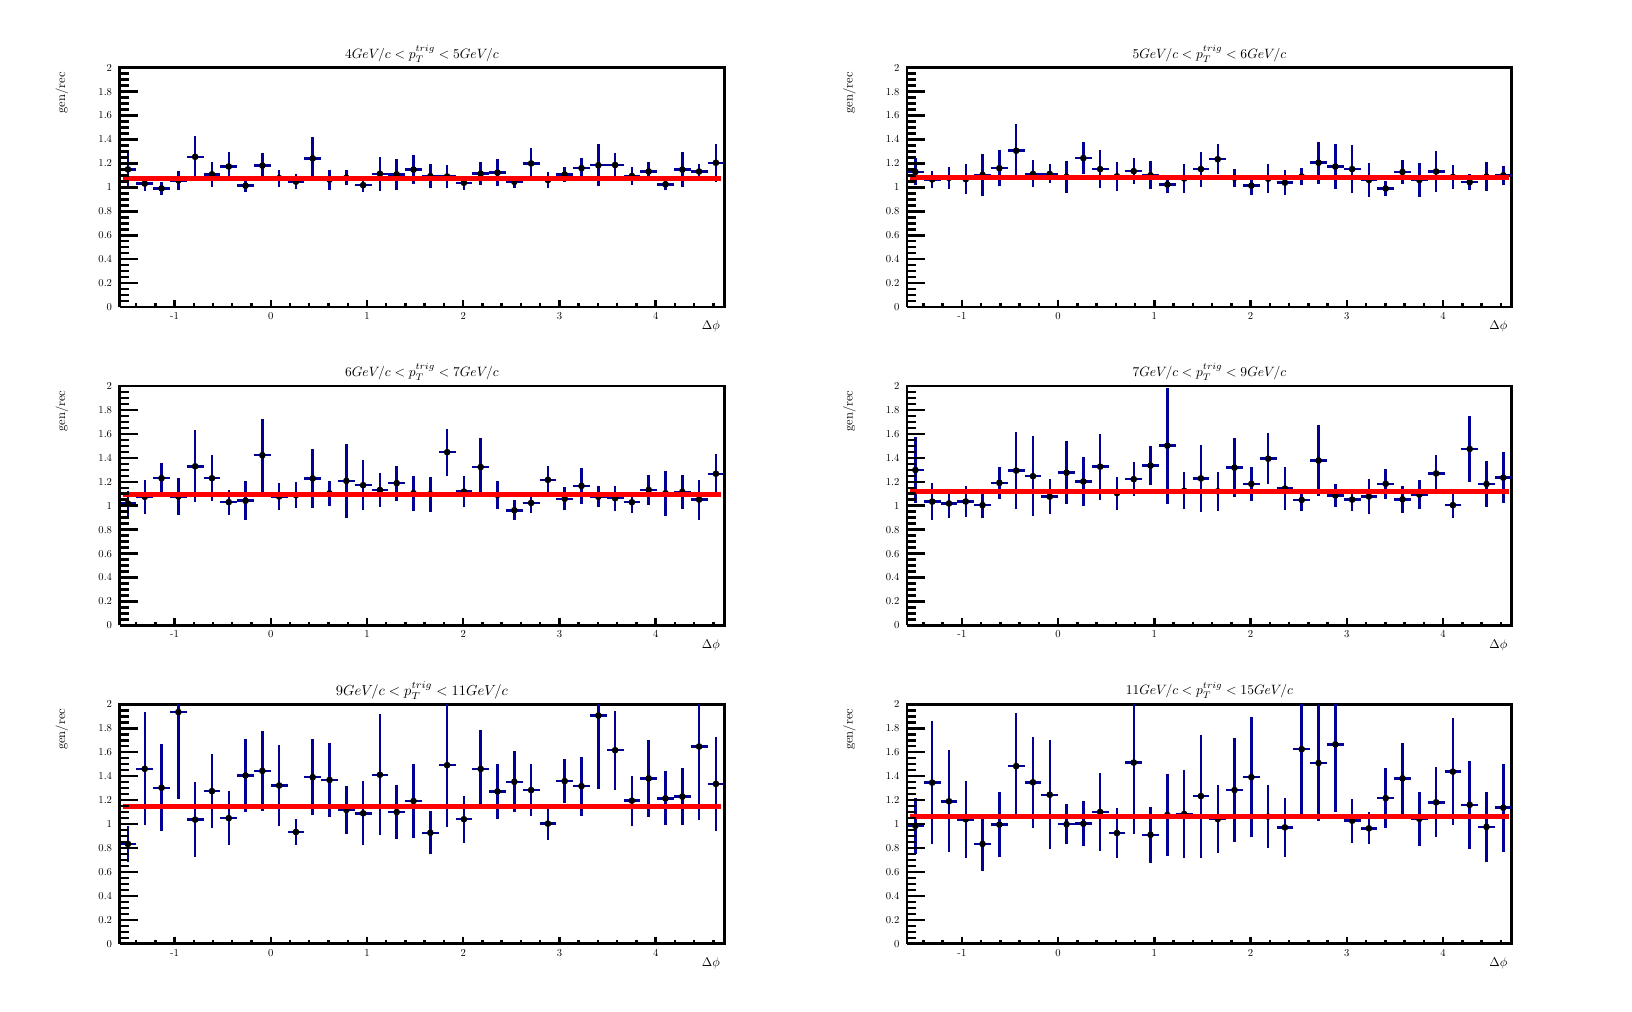
\begin{tikzpicture}
\pgfdeclareplotmark{cross} {
\pgfpathmoveto{\pgfpoint{-0.3\pgfplotmarksize}{\pgfplotmarksize}}
\pgfpathlineto{\pgfpoint{+0.3\pgfplotmarksize}{\pgfplotmarksize}}
\pgfpathlineto{\pgfpoint{+0.3\pgfplotmarksize}{0.3\pgfplotmarksize}}
\pgfpathlineto{\pgfpoint{+1\pgfplotmarksize}{0.3\pgfplotmarksize}}
\pgfpathlineto{\pgfpoint{+1\pgfplotmarksize}{-0.3\pgfplotmarksize}}
\pgfpathlineto{\pgfpoint{+0.3\pgfplotmarksize}{-0.3\pgfplotmarksize}}
\pgfpathlineto{\pgfpoint{+0.3\pgfplotmarksize}{-1.\pgfplotmarksize}}
\pgfpathlineto{\pgfpoint{-0.3\pgfplotmarksize}{-1.\pgfplotmarksize}}
\pgfpathlineto{\pgfpoint{-0.3\pgfplotmarksize}{-0.3\pgfplotmarksize}}
\pgfpathlineto{\pgfpoint{-1.\pgfplotmarksize}{-0.3\pgfplotmarksize}}
\pgfpathlineto{\pgfpoint{-1.\pgfplotmarksize}{0.3\pgfplotmarksize}}
\pgfpathlineto{\pgfpoint{-0.3\pgfplotmarksize}{0.3\pgfplotmarksize}}
\pgfpathclose
\pgfusepathqstroke
}
\pgfdeclareplotmark{cross*} {
\pgfpathmoveto{\pgfpoint{-0.3\pgfplotmarksize}{\pgfplotmarksize}}
\pgfpathlineto{\pgfpoint{+0.3\pgfplotmarksize}{\pgfplotmarksize}}
\pgfpathlineto{\pgfpoint{+0.3\pgfplotmarksize}{0.3\pgfplotmarksize}}
\pgfpathlineto{\pgfpoint{+1\pgfplotmarksize}{0.3\pgfplotmarksize}}
\pgfpathlineto{\pgfpoint{+1\pgfplotmarksize}{-0.3\pgfplotmarksize}}
\pgfpathlineto{\pgfpoint{+0.3\pgfplotmarksize}{-0.3\pgfplotmarksize}}
\pgfpathlineto{\pgfpoint{+0.3\pgfplotmarksize}{-1.\pgfplotmarksize}}
\pgfpathlineto{\pgfpoint{-0.3\pgfplotmarksize}{-1.\pgfplotmarksize}}
\pgfpathlineto{\pgfpoint{-0.3\pgfplotmarksize}{-0.3\pgfplotmarksize}}
\pgfpathlineto{\pgfpoint{-1.\pgfplotmarksize}{-0.3\pgfplotmarksize}}
\pgfpathlineto{\pgfpoint{-1.\pgfplotmarksize}{0.3\pgfplotmarksize}}
\pgfpathlineto{\pgfpoint{-0.3\pgfplotmarksize}{0.3\pgfplotmarksize}}
\pgfpathclose
\pgfusepathqfillstroke
}
\pgfdeclareplotmark{newstar} {
\pgfpathmoveto{\pgfqpoint{0pt}{\pgfplotmarksize}}
\pgfpathlineto{\pgfqpointpolar{44}{0.5\pgfplotmarksize}}
\pgfpathlineto{\pgfqpointpolar{18}{\pgfplotmarksize}}
\pgfpathlineto{\pgfqpointpolar{-20}{0.5\pgfplotmarksize}}
\pgfpathlineto{\pgfqpointpolar{-54}{\pgfplotmarksize}}
\pgfpathlineto{\pgfqpointpolar{-90}{0.5\pgfplotmarksize}}
\pgfpathlineto{\pgfqpointpolar{234}{\pgfplotmarksize}}
\pgfpathlineto{\pgfqpointpolar{198}{0.5\pgfplotmarksize}}
\pgfpathlineto{\pgfqpointpolar{162}{\pgfplotmarksize}}
\pgfpathlineto{\pgfqpointpolar{134}{0.5\pgfplotmarksize}}
\pgfpathclose
\pgfusepathqstroke
}
\pgfdeclareplotmark{newstar*} {
\pgfpathmoveto{\pgfqpoint{0pt}{\pgfplotmarksize}}
\pgfpathlineto{\pgfqpointpolar{44}{0.5\pgfplotmarksize}}
\pgfpathlineto{\pgfqpointpolar{18}{\pgfplotmarksize}}
\pgfpathlineto{\pgfqpointpolar{-20}{0.5\pgfplotmarksize}}
\pgfpathlineto{\pgfqpointpolar{-54}{\pgfplotmarksize}}
\pgfpathlineto{\pgfqpointpolar{-90}{0.5\pgfplotmarksize}}
\pgfpathlineto{\pgfqpointpolar{234}{\pgfplotmarksize}}
\pgfpathlineto{\pgfqpointpolar{198}{0.5\pgfplotmarksize}}
\pgfpathlineto{\pgfqpointpolar{162}{\pgfplotmarksize}}
\pgfpathlineto{\pgfqpointpolar{134}{0.5\pgfplotmarksize}}
\pgfpathclose
\pgfusepathqfillstroke
}
\definecolor{c}{rgb}{1,1,1};
\draw [color=c, fill=c] (0,0) rectangle (20,12.1283);
\draw [color=c, fill=c] (0.2,8.20683) rectangle (9.8,12.007);
\draw [color=c, fill=c] (1.16,8.58685) rectangle (8.84,11.627);
\definecolor{c}{rgb}{0,0,0};
\draw [c,line width=0.9] (1.16,8.58685) -- (1.16,11.627) -- (8.84,11.627) -- (8.84,8.58685) -- (1.16,8.58685);
\definecolor{c}{rgb}{1,1,1};
\draw [color=c, fill=c] (1.16,8.58685) rectangle (8.84,11.627);
\definecolor{c}{rgb}{0,0,0};
\draw [c,line width=0.9] (1.16,8.58685) -- (1.16,11.627) -- (8.84,11.627) -- (8.84,8.58685) -- (1.16,8.58685);
\definecolor{c}{rgb}{0,0,0.6};
\draw [c,line width=0.9] (1.26667,10.0849) -- (1.26667,10.3354);
\draw [c,line width=0.9] (1.26667,10.3354) -- (1.26667,10.5858);
\draw [c,line width=0.9] (1.16,10.3354) -- (1.26667,10.3354);
\draw [c,line width=0.9] (1.26667,10.3354) -- (1.37333,10.3354);
\definecolor{c}{rgb}{0,0,0};
\foreach \P in {(1.26667,10.3354)}{\draw[mark options={color=c,fill=c},mark size=2.402402pt,mark=*,mark size=1pt] plot coordinates {\P};}
\definecolor{c}{rgb}{0,0,0.6};
\draw [c,line width=0.9] (1.48,10.0672) -- (1.48,10.1544);
\draw [c,line width=0.9] (1.48,10.1544) -- (1.48,10.2417);
\draw [c,line width=0.9] (1.37333,10.1544) -- (1.48,10.1544);
\draw [c,line width=0.9] (1.48,10.1544) -- (1.58667,10.1544);
\definecolor{c}{rgb}{0,0,0};
\foreach \P in {(1.48,10.1544)}{\draw[mark options={color=c,fill=c},mark size=2.402402pt,mark=*,mark size=1pt] plot coordinates {\P};}
\definecolor{c}{rgb}{0,0,0.6};
\draw [c,line width=0.9] (1.69333,10.0148) -- (1.69333,10.0938);
\draw [c,line width=0.9] (1.69333,10.0938) -- (1.69333,10.1729);
\draw [c,line width=0.9] (1.58667,10.0938) -- (1.69333,10.0938);
\draw [c,line width=0.9] (1.69333,10.0938) -- (1.8,10.0938);
\definecolor{c}{rgb}{0,0,0};
\foreach \P in {(1.69333,10.0938)}{\draw[mark options={color=c,fill=c},mark size=2.402402pt,mark=*,mark size=1pt] plot coordinates {\P};}
\definecolor{c}{rgb}{0,0,0.6};
\draw [c,line width=0.9] (1.90667,10.0792) -- (1.90667,10.1966);
\draw [c,line width=0.9] (1.90667,10.1966) -- (1.90667,10.314);
\draw [c,line width=0.9] (1.8,10.1966) -- (1.90667,10.1966);
\draw [c,line width=0.9] (1.90667,10.1966) -- (2.01333,10.1966);
\definecolor{c}{rgb}{0,0,0};
\foreach \P in {(1.90667,10.1966)}{\draw[mark options={color=c,fill=c},mark size=2.402402pt,mark=*,mark size=1pt] plot coordinates {\P};}
\definecolor{c}{rgb}{0,0,0.6};
\draw [c,line width=0.9] (2.12,10.2246) -- (2.12,10.495);
\draw [c,line width=0.9] (2.12,10.495) -- (2.12,10.7653);
\draw [c,line width=0.9] (2.01333,10.495) -- (2.12,10.495);
\draw [c,line width=0.9] (2.12,10.495) -- (2.22667,10.495);
\definecolor{c}{rgb}{0,0,0};
\foreach \P in {(2.12,10.495)}{\draw[mark options={color=c,fill=c},mark size=2.402402pt,mark=*,mark size=1pt] plot coordinates {\P};}
\definecolor{c}{rgb}{0,0,0.6};
\draw [c,line width=0.9] (2.33333,10.1167) -- (2.33333,10.2731);
\draw [c,line width=0.9] (2.33333,10.2731) -- (2.33333,10.4294);
\draw [c,line width=0.9] (2.22667,10.2731) -- (2.33333,10.2731);
\draw [c,line width=0.9] (2.33333,10.2731) -- (2.44,10.2731);
\definecolor{c}{rgb}{0,0,0};
\foreach \P in {(2.33333,10.2731)}{\draw[mark options={color=c,fill=c},mark size=2.402402pt,mark=*,mark size=1pt] plot coordinates {\P};}
\definecolor{c}{rgb}{0,0,0.6};
\draw [c,line width=0.9] (2.54667,10.184) -- (2.54667,10.3721);
\draw [c,line width=0.9] (2.54667,10.3721) -- (2.54667,10.5602);
\draw [c,line width=0.9] (2.44,10.3721) -- (2.54667,10.3721);
\draw [c,line width=0.9] (2.54667,10.3721) -- (2.65333,10.3721);
\definecolor{c}{rgb}{0,0,0};
\foreach \P in {(2.54667,10.3721)}{\draw[mark options={color=c,fill=c},mark size=2.402402pt,mark=*,mark size=1pt] plot coordinates {\P};}
\definecolor{c}{rgb}{0,0,0.6};
\draw [c,line width=0.9] (2.76,10.0521) -- (2.76,10.1283);
\draw [c,line width=0.9] (2.76,10.1283) -- (2.76,10.2046);
\draw [c,line width=0.9] (2.65333,10.1283) -- (2.76,10.1283);
\draw [c,line width=0.9] (2.76,10.1283) -- (2.86667,10.1283);
\definecolor{c}{rgb}{0,0,0};
\foreach \P in {(2.76,10.1283)}{\draw[mark options={color=c,fill=c},mark size=2.402402pt,mark=*,mark size=1pt] plot coordinates {\P};}
\definecolor{c}{rgb}{0,0,0.6};
\draw [c,line width=0.9] (2.97333,10.221) -- (2.97333,10.3829);
\draw [c,line width=0.9] (2.97333,10.3829) -- (2.97333,10.5447);
\draw [c,line width=0.9] (2.86667,10.3829) -- (2.97333,10.3829);
\draw [c,line width=0.9] (2.97333,10.3829) -- (3.08,10.3829);
\definecolor{c}{rgb}{0,0,0};
\foreach \P in {(2.97333,10.3829)}{\draw[mark options={color=c,fill=c},mark size=2.402402pt,mark=*,mark size=1pt] plot coordinates {\P};}
\definecolor{c}{rgb}{0,0,0.6};
\draw [c,line width=0.9] (3.18667,10.1153) -- (3.18667,10.2246);
\draw [c,line width=0.9] (3.18667,10.2246) -- (3.18667,10.3338);
\draw [c,line width=0.9] (3.08,10.2246) -- (3.18667,10.2246);
\draw [c,line width=0.9] (3.18667,10.2246) -- (3.29333,10.2246);
\definecolor{c}{rgb}{0,0,0};
\foreach \P in {(3.18667,10.2246)}{\draw[mark options={color=c,fill=c},mark size=2.402402pt,mark=*,mark size=1pt] plot coordinates {\P};}
\definecolor{c}{rgb}{0,0,0.6};
\draw [c,line width=0.9] (3.4,10.0813) -- (3.4,10.1787);
\draw [c,line width=0.9] (3.4,10.1787) -- (3.4,10.2761);
\draw [c,line width=0.9] (3.29333,10.1787) -- (3.4,10.1787);
\draw [c,line width=0.9] (3.4,10.1787) -- (3.50667,10.1787);
\definecolor{c}{rgb}{0,0,0};
\foreach \P in {(3.4,10.1787)}{\draw[mark options={color=c,fill=c},mark size=2.402402pt,mark=*,mark size=1pt] plot coordinates {\P};}
\definecolor{c}{rgb}{0,0,0.6};
\draw [c,line width=0.9] (3.61333,10.2004) -- (3.61333,10.4757);
\draw [c,line width=0.9] (3.61333,10.4757) -- (3.61333,10.7511);
\draw [c,line width=0.9] (3.50667,10.4757) -- (3.61333,10.4757);
\draw [c,line width=0.9] (3.61333,10.4757) -- (3.72,10.4757);
\definecolor{c}{rgb}{0,0,0};
\foreach \P in {(3.61333,10.4757)}{\draw[mark options={color=c,fill=c},mark size=2.402402pt,mark=*,mark size=1pt] plot coordinates {\P};}
\definecolor{c}{rgb}{0,0,0.6};
\draw [c,line width=0.9] (3.82667,10.0799) -- (3.82667,10.2054);
\draw [c,line width=0.9] (3.82667,10.2054) -- (3.82667,10.331);
\draw [c,line width=0.9] (3.72,10.2054) -- (3.82667,10.2054);
\draw [c,line width=0.9] (3.82667,10.2054) -- (3.93333,10.2054);
\definecolor{c}{rgb}{0,0,0};
\foreach \P in {(3.82667,10.2054)}{\draw[mark options={color=c,fill=c},mark size=2.402402pt,mark=*,mark size=1pt] plot coordinates {\P};}
\definecolor{c}{rgb}{0,0,0.6};
\draw [c,line width=0.9] (4.04,10.1323) -- (4.04,10.2283);
\draw [c,line width=0.9] (4.04,10.2283) -- (4.04,10.3244);
\draw [c,line width=0.9] (3.93333,10.2283) -- (4.04,10.2283);
\draw [c,line width=0.9] (4.04,10.2283) -- (4.14667,10.2283);
\definecolor{c}{rgb}{0,0,0};
\foreach \P in {(4.04,10.2283)}{\draw[mark options={color=c,fill=c},mark size=2.402402pt,mark=*,mark size=1pt] plot coordinates {\P};}
\definecolor{c}{rgb}{0,0,0.6};
\draw [c,line width=0.9] (4.25333,10.0472) -- (4.25333,10.1354);
\draw [c,line width=0.9] (4.25333,10.1354) -- (4.25333,10.2237);
\draw [c,line width=0.9] (4.14667,10.1354) -- (4.25333,10.1354);
\draw [c,line width=0.9] (4.25333,10.1354) -- (4.36,10.1354);
\definecolor{c}{rgb}{0,0,0};
\foreach \P in {(4.25333,10.1354)}{\draw[mark options={color=c,fill=c},mark size=2.402402pt,mark=*,mark size=1pt] plot coordinates {\P};}
\definecolor{c}{rgb}{0,0,0.6};
\draw [c,line width=0.9] (4.46667,10.066) -- (4.46667,10.2794);
\draw [c,line width=0.9] (4.46667,10.2794) -- (4.46667,10.4929);
\draw [c,line width=0.9] (4.36,10.2794) -- (4.46667,10.2794);
\draw [c,line width=0.9] (4.46667,10.2794) -- (4.57333,10.2794);
\definecolor{c}{rgb}{0,0,0};
\foreach \P in {(4.46667,10.2794)}{\draw[mark options={color=c,fill=c},mark size=2.402402pt,mark=*,mark size=1pt] plot coordinates {\P};}
\definecolor{c}{rgb}{0,0,0.6};
\draw [c,line width=0.9] (4.68,10.0731) -- (4.68,10.2727);
\draw [c,line width=0.9] (4.68,10.2727) -- (4.68,10.4723);
\draw [c,line width=0.9] (4.57333,10.2727) -- (4.68,10.2727);
\draw [c,line width=0.9] (4.68,10.2727) -- (4.78667,10.2727);
\definecolor{c}{rgb}{0,0,0};
\foreach \P in {(4.68,10.2727)}{\draw[mark options={color=c,fill=c},mark size=2.402402pt,mark=*,mark size=1pt] plot coordinates {\P};}
\definecolor{c}{rgb}{0,0,0.6};
\draw [c,line width=0.9] (4.89333,10.1468) -- (4.89333,10.3325);
\draw [c,line width=0.9] (4.89333,10.3325) -- (4.89333,10.5182);
\draw [c,line width=0.9] (4.78667,10.3325) -- (4.89333,10.3325);
\draw [c,line width=0.9] (4.89333,10.3325) -- (5,10.3325);
\definecolor{c}{rgb}{0,0,0};
\foreach \P in {(4.89333,10.3325)}{\draw[mark options={color=c,fill=c},mark size=2.402402pt,mark=*,mark size=1pt] plot coordinates {\P};}
\definecolor{c}{rgb}{0,0,0.6};
\draw [c,line width=0.9] (5.10667,10.0978) -- (5.10667,10.2493);
\draw [c,line width=0.9] (5.10667,10.2493) -- (5.10667,10.4009);
\draw [c,line width=0.9] (5,10.2493) -- (5.10667,10.2493);
\draw [c,line width=0.9] (5.10667,10.2493) -- (5.21333,10.2493);
\definecolor{c}{rgb}{0,0,0};
\foreach \P in {(5.10667,10.2493)}{\draw[mark options={color=c,fill=c},mark size=2.402402pt,mark=*,mark size=1pt] plot coordinates {\P};}
\definecolor{c}{rgb}{0,0,0.6};
\draw [c,line width=0.9] (5.32,10.1048) -- (5.32,10.2457);
\draw [c,line width=0.9] (5.32,10.2457) -- (5.32,10.3867);
\draw [c,line width=0.9] (5.21333,10.2457) -- (5.32,10.2457);
\draw [c,line width=0.9] (5.32,10.2457) -- (5.42667,10.2457);
\definecolor{c}{rgb}{0,0,0};
\foreach \P in {(5.32,10.2457)}{\draw[mark options={color=c,fill=c},mark size=2.402402pt,mark=*,mark size=1pt] plot coordinates {\P};}
\definecolor{c}{rgb}{0,0,0.6};
\draw [c,line width=0.9] (5.53333,10.0767) -- (5.53333,10.1655);
\draw [c,line width=0.9] (5.53333,10.1655) -- (5.53333,10.2543);
\draw [c,line width=0.9] (5.42667,10.1655) -- (5.53333,10.1655);
\draw [c,line width=0.9] (5.53333,10.1655) -- (5.64,10.1655);
\definecolor{c}{rgb}{0,0,0};
\foreach \P in {(5.53333,10.1655)}{\draw[mark options={color=c,fill=c},mark size=2.402402pt,mark=*,mark size=1pt] plot coordinates {\P};}
\definecolor{c}{rgb}{0,0,0.6};
\draw [c,line width=0.9] (5.74667,10.137) -- (5.74667,10.2803);
\draw [c,line width=0.9] (5.74667,10.2803) -- (5.74667,10.4237);
\draw [c,line width=0.9] (5.64,10.2803) -- (5.74667,10.2803);
\draw [c,line width=0.9] (5.74667,10.2803) -- (5.85333,10.2803);
\definecolor{c}{rgb}{0,0,0};
\foreach \P in {(5.74667,10.2803)}{\draw[mark options={color=c,fill=c},mark size=2.402402pt,mark=*,mark size=1pt] plot coordinates {\P};}
\definecolor{c}{rgb}{0,0,0.6};
\draw [c,line width=0.9] (5.96,10.1244) -- (5.96,10.2945);
\draw [c,line width=0.9] (5.96,10.2945) -- (5.96,10.4645);
\draw [c,line width=0.9] (5.85333,10.2945) -- (5.96,10.2945);
\draw [c,line width=0.9] (5.96,10.2945) -- (6.06667,10.2945);
\definecolor{c}{rgb}{0,0,0};
\foreach \P in {(5.96,10.2945)}{\draw[mark options={color=c,fill=c},mark size=2.402402pt,mark=*,mark size=1pt] plot coordinates {\P};}
\definecolor{c}{rgb}{0,0,0.6};
\draw [c,line width=0.9] (6.17333,10.1042) -- (6.17333,10.1769);
\draw [c,line width=0.9] (6.17333,10.1769) -- (6.17333,10.2496);
\draw [c,line width=0.9] (6.06667,10.1769) -- (6.17333,10.1769);
\draw [c,line width=0.9] (6.17333,10.1769) -- (6.28,10.1769);
\definecolor{c}{rgb}{0,0,0};
\foreach \P in {(6.17333,10.1769)}{\draw[mark options={color=c,fill=c},mark size=2.402402pt,mark=*,mark size=1pt] plot coordinates {\P};}
\definecolor{c}{rgb}{0,0,0.6};
\draw [c,line width=0.9] (6.38667,10.22) -- (6.38667,10.4111);
\draw [c,line width=0.9] (6.38667,10.4111) -- (6.38667,10.6021);
\draw [c,line width=0.9] (6.28,10.4111) -- (6.38667,10.4111);
\draw [c,line width=0.9] (6.38667,10.4111) -- (6.49333,10.4111);
\definecolor{c}{rgb}{0,0,0};
\foreach \P in {(6.38667,10.4111)}{\draw[mark options={color=c,fill=c},mark size=2.402402pt,mark=*,mark size=1pt] plot coordinates {\P};}
\definecolor{c}{rgb}{0,0,0.6};
\draw [c,line width=0.9] (6.6,10.0995) -- (6.6,10.1997);
\draw [c,line width=0.9] (6.6,10.1997) -- (6.6,10.2998);
\draw [c,line width=0.9] (6.49333,10.1997) -- (6.6,10.1997);
\draw [c,line width=0.9] (6.6,10.1997) -- (6.70667,10.1997);
\definecolor{c}{rgb}{0,0,0};
\foreach \P in {(6.6,10.1997)}{\draw[mark options={color=c,fill=c},mark size=2.402402pt,mark=*,mark size=1pt] plot coordinates {\P};}
\definecolor{c}{rgb}{0,0,0.6};
\draw [c,line width=0.9] (6.81333,10.1807) -- (6.81333,10.2707);
\draw [c,line width=0.9] (6.81333,10.2707) -- (6.81333,10.3607);
\draw [c,line width=0.9] (6.70667,10.2707) -- (6.81333,10.2707);
\draw [c,line width=0.9] (6.81333,10.2707) -- (6.92,10.2707);
\definecolor{c}{rgb}{0,0,0};
\foreach \P in {(6.81333,10.2707)}{\draw[mark options={color=c,fill=c},mark size=2.402402pt,mark=*,mark size=1pt] plot coordinates {\P};}
\definecolor{c}{rgb}{0,0,0.6};
\draw [c,line width=0.9] (7.02667,10.223) -- (7.02667,10.3513);
\draw [c,line width=0.9] (7.02667,10.3513) -- (7.02667,10.4796);
\draw [c,line width=0.9] (6.92,10.3513) -- (7.02667,10.3513);
\draw [c,line width=0.9] (7.02667,10.3513) -- (7.13333,10.3513);
\definecolor{c}{rgb}{0,0,0};
\foreach \P in {(7.02667,10.3513)}{\draw[mark options={color=c,fill=c},mark size=2.402402pt,mark=*,mark size=1pt] plot coordinates {\P};}
\definecolor{c}{rgb}{0,0,0.6};
\draw [c,line width=0.9] (7.24,10.122) -- (7.24,10.3881);
\draw [c,line width=0.9] (7.24,10.3881) -- (7.24,10.6542);
\draw [c,line width=0.9] (7.13333,10.3881) -- (7.24,10.3881);
\draw [c,line width=0.9] (7.24,10.3881) -- (7.34667,10.3881);
\definecolor{c}{rgb}{0,0,0};
\foreach \P in {(7.24,10.3881)}{\draw[mark options={color=c,fill=c},mark size=2.402402pt,mark=*,mark size=1pt] plot coordinates {\P};}
\definecolor{c}{rgb}{0,0,0.6};
\draw [c,line width=0.9] (7.45333,10.2445) -- (7.45333,10.3914);
\draw [c,line width=0.9] (7.45333,10.3914) -- (7.45333,10.5384);
\draw [c,line width=0.9] (7.34667,10.3914) -- (7.45333,10.3914);
\draw [c,line width=0.9] (7.45333,10.3914) -- (7.56,10.3914);
\definecolor{c}{rgb}{0,0,0};
\foreach \P in {(7.45333,10.3914)}{\draw[mark options={color=c,fill=c},mark size=2.402402pt,mark=*,mark size=1pt] plot coordinates {\P};}
\definecolor{c}{rgb}{0,0,0.6};
\draw [c,line width=0.9] (7.66667,10.1367) -- (7.66667,10.2508);
\draw [c,line width=0.9] (7.66667,10.2508) -- (7.66667,10.365);
\draw [c,line width=0.9] (7.56,10.2508) -- (7.66667,10.2508);
\draw [c,line width=0.9] (7.66667,10.2508) -- (7.77333,10.2508);
\definecolor{c}{rgb}{0,0,0};
\foreach \P in {(7.66667,10.2508)}{\draw[mark options={color=c,fill=c},mark size=2.402402pt,mark=*,mark size=1pt] plot coordinates {\P};}
\definecolor{c}{rgb}{0,0,0.6};
\draw [c,line width=0.9] (7.88,10.1896) -- (7.88,10.3091);
\draw [c,line width=0.9] (7.88,10.3091) -- (7.88,10.4285);
\draw [c,line width=0.9] (7.77333,10.3091) -- (7.88,10.3091);
\draw [c,line width=0.9] (7.88,10.3091) -- (7.98667,10.3091);
\definecolor{c}{rgb}{0,0,0};
\foreach \P in {(7.88,10.3091)}{\draw[mark options={color=c,fill=c},mark size=2.402402pt,mark=*,mark size=1pt] plot coordinates {\P};}
\definecolor{c}{rgb}{0,0,0.6};
\draw [c,line width=0.9] (8.09333,10.0719) -- (8.09333,10.1463);
\draw [c,line width=0.9] (8.09333,10.1463) -- (8.09333,10.2206);
\draw [c,line width=0.9] (7.98667,10.1463) -- (8.09333,10.1463);
\draw [c,line width=0.9] (8.09333,10.1463) -- (8.2,10.1463);
\definecolor{c}{rgb}{0,0,0};
\foreach \P in {(8.09333,10.1463)}{\draw[mark options={color=c,fill=c},mark size=2.402402pt,mark=*,mark size=1pt] plot coordinates {\P};}
\definecolor{c}{rgb}{0,0,0.6};
\draw [c,line width=0.9] (8.30667,10.1132) -- (8.30667,10.3328);
\draw [c,line width=0.9] (8.30667,10.3328) -- (8.30667,10.5524);
\draw [c,line width=0.9] (8.2,10.3328) -- (8.30667,10.3328);
\draw [c,line width=0.9] (8.30667,10.3328) -- (8.41333,10.3328);
\definecolor{c}{rgb}{0,0,0};
\foreach \P in {(8.30667,10.3328)}{\draw[mark options={color=c,fill=c},mark size=2.402402pt,mark=*,mark size=1pt] plot coordinates {\P};}
\definecolor{c}{rgb}{0,0,0.6};
\draw [c,line width=0.9] (8.52,10.2149) -- (8.52,10.3085);
\draw [c,line width=0.9] (8.52,10.3085) -- (8.52,10.402);
\draw [c,line width=0.9] (8.41333,10.3085) -- (8.52,10.3085);
\draw [c,line width=0.9] (8.52,10.3085) -- (8.62667,10.3085);
\definecolor{c}{rgb}{0,0,0};
\foreach \P in {(8.52,10.3085)}{\draw[mark options={color=c,fill=c},mark size=2.402402pt,mark=*,mark size=1pt] plot coordinates {\P};}
\definecolor{c}{rgb}{0,0,0.6};
\draw [c,line width=0.9] (8.73333,10.1754) -- (8.73333,10.4194);
\draw [c,line width=0.9] (8.73333,10.4194) -- (8.73333,10.6634);
\draw [c,line width=0.9] (8.62667,10.4194) -- (8.73333,10.4194);
\draw [c,line width=0.9] (8.73333,10.4194) -- (8.84,10.4194);
\definecolor{c}{rgb}{0,0,0};
\foreach \P in {(8.73333,10.4194)}{\draw[mark options={color=c,fill=c},mark size=2.402402pt,mark=*,mark size=1pt] plot coordinates {\P};}
\definecolor{c}{rgb}{1,0,0};
\draw [c,line width=1.8] (1.1984,10.2193) -- (1.2752,10.2193) -- (1.352,10.2193) -- (1.4288,10.2193) -- (1.5056,10.2193) -- (1.5824,10.2193) -- (1.6592,10.2193) -- (1.736,10.2193) -- (1.8128,10.2193) -- (1.8896,10.2193) -- (1.9664,10.2193) --
 (2.0432,10.2193) -- (2.12,10.2193) -- (2.1968,10.2193) -- (2.2736,10.2193) -- (2.3504,10.2193) -- (2.4272,10.2193) -- (2.504,10.2193) -- (2.5808,10.2193) -- (2.6576,10.2193) -- (2.7344,10.2193) -- (2.8112,10.2193) -- (2.888,10.2193) --
 (2.9648,10.2193) -- (3.0416,10.2193) -- (3.1184,10.2193) -- (3.1952,10.2193) -- (3.272,10.2193) -- (3.3488,10.2193) -- (3.4256,10.2193) -- (3.5024,10.2193) -- (3.5792,10.2193) -- (3.656,10.2193) -- (3.7328,10.2193) -- (3.8096,10.2193) --
 (3.8864,10.2193) -- (3.9632,10.2193) -- (4.04,10.2193) -- (4.1168,10.2193) -- (4.1936,10.2193) -- (4.2704,10.2193) -- (4.3472,10.2193) -- (4.424,10.2193) -- (4.5008,10.2193) -- (4.5776,10.2193) -- (4.6544,10.2193) -- (4.7312,10.2193) --
 (4.808,10.2193) -- (4.8848,10.2193) -- (4.9616,10.2193);
\draw [c,line width=1.8] (4.9616,10.2193) -- (5.0384,10.2193) -- (5.1152,10.2193) -- (5.192,10.2193) -- (5.2688,10.2193) -- (5.3456,10.2193) -- (5.4224,10.2193) -- (5.4992,10.2193) -- (5.576,10.2193) -- (5.6528,10.2193) -- (5.7296,10.2193) --
 (5.8064,10.2193) -- (5.8832,10.2193) -- (5.96,10.2193) -- (6.0368,10.2193) -- (6.1136,10.2193) -- (6.1904,10.2193) -- (6.2672,10.2193) -- (6.344,10.2193) -- (6.4208,10.2193) -- (6.4976,10.2193) -- (6.5744,10.2193) -- (6.6512,10.2193) --
 (6.728,10.2193) -- (6.8048,10.2193) -- (6.8816,10.2193) -- (6.9584,10.2193) -- (7.0352,10.2193) -- (7.112,10.2193) -- (7.1888,10.2193) -- (7.2656,10.2193) -- (7.3424,10.2193) -- (7.4192,10.2193) -- (7.496,10.2193) -- (7.5728,10.2193) --
 (7.6496,10.2193) -- (7.7264,10.2193) -- (7.8032,10.2193) -- (7.88,10.2193) -- (7.9568,10.2193) -- (8.0336,10.2193) -- (8.1104,10.2193) -- (8.1872,10.2193) -- (8.264,10.2193) -- (8.3408,10.2193) -- (8.4176,10.2193) -- (8.4944,10.2193) --
 (8.5712,10.2193) -- (8.648,10.2193) -- (8.7248,10.2193);
\draw [c,line width=1.8] (8.7248,10.2193) -- (8.8016,10.2193);
\definecolor{c}{rgb}{0,0,0};
\draw [c,line width=0.9] (1.16,8.58685) -- (8.84,8.58685);
\draw [c,line width=0.9] (1.85769,8.67806) -- (1.85769,8.58685);
\draw [c,line width=0.9] (2.10215,8.63246) -- (2.10215,8.58685);
\draw [c,line width=0.9] (2.34661,8.63246) -- (2.34661,8.58685);
\draw [c,line width=0.9] (2.59108,8.63246) -- (2.59108,8.58685);
\draw [c,line width=0.9] (2.83554,8.63246) -- (2.83554,8.58685);
\draw [c,line width=0.9] (3.08,8.67806) -- (3.08,8.58685);
\draw [c,line width=0.9] (3.32446,8.63246) -- (3.32446,8.58685);
\draw [c,line width=0.9] (3.56892,8.63246) -- (3.56892,8.58685);
\draw [c,line width=0.9] (3.81339,8.63246) -- (3.81339,8.58685);
\draw [c,line width=0.9] (4.05785,8.63246) -- (4.05785,8.58685);
\draw [c,line width=0.9] (4.30231,8.67806) -- (4.30231,8.58685);
\draw [c,line width=0.9] (4.54677,8.63246) -- (4.54677,8.58685);
\draw [c,line width=0.9] (4.79123,8.63246) -- (4.79123,8.58685);
\draw [c,line width=0.9] (5.0357,8.63246) -- (5.0357,8.58685);
\draw [c,line width=0.9] (5.28016,8.63246) -- (5.28016,8.58685);
\draw [c,line width=0.9] (5.52462,8.67806) -- (5.52462,8.58685);
\draw [c,line width=0.9] (5.76908,8.63246) -- (5.76908,8.58685);
\draw [c,line width=0.9] (6.01354,8.63246) -- (6.01354,8.58685);
\draw [c,line width=0.9] (6.25801,8.63246) -- (6.25801,8.58685);
\draw [c,line width=0.9] (6.50247,8.63246) -- (6.50247,8.58685);
\draw [c,line width=0.9] (6.74693,8.67806) -- (6.74693,8.58685);
\draw [c,line width=0.9] (6.99139,8.63246) -- (6.99139,8.58685);
\draw [c,line width=0.9] (7.23585,8.63246) -- (7.23585,8.58685);
\draw [c,line width=0.9] (7.48032,8.63246) -- (7.48032,8.58685);
\draw [c,line width=0.9] (7.72478,8.63246) -- (7.72478,8.58685);
\draw [c,line width=0.9] (7.96924,8.67806) -- (7.96924,8.58685);
\draw [c,line width=0.9] (1.85769,8.67806) -- (1.85769,8.58685);
\draw [c,line width=0.9] (1.61323,8.63246) -- (1.61323,8.58685);
\draw [c,line width=0.9] (1.36877,8.63246) -- (1.36877,8.58685);
\draw [c,line width=0.9] (7.96924,8.67806) -- (7.96924,8.58685);
\draw [c,line width=0.9] (8.2137,8.63246) -- (8.2137,8.58685);
\draw [c,line width=0.9] (8.45816,8.63246) -- (8.45816,8.58685);
\draw [c,line width=0.9] (8.70263,8.63246) -- (8.70263,8.58685);
\draw [anchor=base] (1.85769,8.43105) node[scale=0.383643, color=c, rotate=0]{-1};
\draw [anchor=base] (3.08,8.43105) node[scale=0.383643, color=c, rotate=0]{0};
\draw [anchor=base] (4.30231,8.43105) node[scale=0.383643, color=c, rotate=0]{1};
\draw [anchor=base] (5.52462,8.43105) node[scale=0.383643, color=c, rotate=0]{2};
\draw [anchor=base] (6.74693,8.43105) node[scale=0.383643, color=c, rotate=0]{3};
\draw [anchor=base] (7.96924,8.43105) node[scale=0.383643, color=c, rotate=0]{4};
\draw [anchor= east] (8.84,8.33604) node[scale=0.453396, color=c, rotate=0]{$\Delta \phi$};
\draw [c,line width=0.9] (1.16,8.58685) -- (1.16,11.627);
\draw [c,line width=0.9] (1.3904,8.58685) -- (1.16,8.58685);
\draw [c,line width=0.9] (1.2752,8.66286) -- (1.16,8.66286);
\draw [c,line width=0.9] (1.2752,8.73886) -- (1.16,8.73886);
\draw [c,line width=0.9] (1.2752,8.81487) -- (1.16,8.81487);
\draw [c,line width=0.9] (1.3904,8.89087) -- (1.16,8.89087);
\draw [c,line width=0.9] (1.2752,8.96688) -- (1.16,8.96688);
\draw [c,line width=0.9] (1.2752,9.04288) -- (1.16,9.04288);
\draw [c,line width=0.9] (1.2752,9.11888) -- (1.16,9.11888);
\draw [c,line width=0.9] (1.3904,9.19489) -- (1.16,9.19489);
\draw [c,line width=0.9] (1.2752,9.27089) -- (1.16,9.27089);
\draw [c,line width=0.9] (1.2752,9.3469) -- (1.16,9.3469);
\draw [c,line width=0.9] (1.2752,9.4229) -- (1.16,9.4229);
\draw [c,line width=0.9] (1.3904,9.4989) -- (1.16,9.4989);
\draw [c,line width=0.9] (1.2752,9.57491) -- (1.16,9.57491);
\draw [c,line width=0.9] (1.2752,9.65091) -- (1.16,9.65091);
\draw [c,line width=0.9] (1.2752,9.72692) -- (1.16,9.72692);
\draw [c,line width=0.9] (1.3904,9.80292) -- (1.16,9.80292);
\draw [c,line width=0.9] (1.2752,9.87893) -- (1.16,9.87893);
\draw [c,line width=0.9] (1.2752,9.95493) -- (1.16,9.95493);
\draw [c,line width=0.9] (1.2752,10.0309) -- (1.16,10.0309);
\draw [c,line width=0.9] (1.3904,10.1069) -- (1.16,10.1069);
\draw [c,line width=0.9] (1.2752,10.1829) -- (1.16,10.1829);
\draw [c,line width=0.9] (1.2752,10.2589) -- (1.16,10.2589);
\draw [c,line width=0.9] (1.2752,10.335) -- (1.16,10.335);
\draw [c,line width=0.9] (1.3904,10.411) -- (1.16,10.411);
\draw [c,line width=0.9] (1.2752,10.487) -- (1.16,10.487);
\draw [c,line width=0.9] (1.2752,10.563) -- (1.16,10.563);
\draw [c,line width=0.9] (1.2752,10.639) -- (1.16,10.639);
\draw [c,line width=0.9] (1.3904,10.715) -- (1.16,10.715);
\draw [c,line width=0.9] (1.2752,10.791) -- (1.16,10.791);
\draw [c,line width=0.9] (1.2752,10.867) -- (1.16,10.867);
\draw [c,line width=0.9] (1.2752,10.943) -- (1.16,10.943);
\draw [c,line width=0.9] (1.3904,11.019) -- (1.16,11.019);
\draw [c,line width=0.9] (1.2752,11.095) -- (1.16,11.095);
\draw [c,line width=0.9] (1.2752,11.171) -- (1.16,11.171);
\draw [c,line width=0.9] (1.2752,11.247) -- (1.16,11.247);
\draw [c,line width=0.9] (1.3904,11.323) -- (1.16,11.323);
\draw [c,line width=0.9] (1.2752,11.399) -- (1.16,11.399);
\draw [c,line width=0.9] (1.2752,11.475) -- (1.16,11.475);
\draw [c,line width=0.9] (1.2752,11.551) -- (1.16,11.551);
\draw [c,line width=0.9] (1.3904,11.627) -- (1.16,11.627);
\draw [anchor= east] (1.112,8.58685) node[scale=0.383643, color=c, rotate=0]{0};
\draw [anchor= east] (1.112,8.89087) node[scale=0.383643, color=c, rotate=0]{0.2};
\draw [anchor= east] (1.112,9.19489) node[scale=0.383643, color=c, rotate=0]{0.4};
\draw [anchor= east] (1.112,9.4989) node[scale=0.383643, color=c, rotate=0]{0.6};
\draw [anchor= east] (1.112,9.80292) node[scale=0.383643, color=c, rotate=0]{0.8};
\draw [anchor= east] (1.112,10.1069) node[scale=0.383643, color=c, rotate=0]{1};
\draw [anchor= east] (1.112,10.411) node[scale=0.383643, color=c, rotate=0]{1.2};
\draw [anchor= east] (1.112,10.715) node[scale=0.383643, color=c, rotate=0]{1.4};
\draw [anchor= east] (1.112,11.019) node[scale=0.383643, color=c, rotate=0]{1.6};
\draw [anchor= east] (1.112,11.323) node[scale=0.383643, color=c, rotate=0]{1.8};
\draw [anchor= east] (1.112,11.627) node[scale=0.383643, color=c, rotate=0]{2};
\draw [anchor= east] (0.428557,11.627) node[scale=0.453396, color=c, rotate=90]{gen/rec};
\draw (5,11.8042) node[scale=0.488273, color=c, rotate=0]{$4 GeV/c < p_{T}^{trig} < 5 GeV/c$};
\definecolor{c}{rgb}{1,1,1};
\draw [color=c, fill=c] (10.2,8.20683) rectangle (19.8,12.007);
\draw [color=c, fill=c] (11.16,8.58685) rectangle (18.84,11.627);
\definecolor{c}{rgb}{0,0,0};
\draw [c,line width=0.9] (11.16,8.58685) -- (11.16,11.627) -- (18.84,11.627) -- (18.84,8.58685) -- (11.16,8.58685);
\definecolor{c}{rgb}{1,1,1};
\draw [color=c, fill=c] (11.16,8.58685) rectangle (18.84,11.627);
\definecolor{c}{rgb}{0,0,0};
\draw [c,line width=0.9] (11.16,8.58685) -- (11.16,11.627) -- (18.84,11.627) -- (18.84,8.58685) -- (11.16,8.58685);
\definecolor{c}{rgb}{0,0,0.6};
\draw [c,line width=0.9] (11.2667,10.1322) -- (11.2667,10.3036);
\draw [c,line width=0.9] (11.2667,10.3036) -- (11.2667,10.4749);
\draw [c,line width=0.9] (11.16,10.3036) -- (11.2667,10.3036);
\draw [c,line width=0.9] (11.2667,10.3036) -- (11.3733,10.3036);
\definecolor{c}{rgb}{0,0,0};
\foreach \P in {(11.2667,10.3036)}{\draw[mark options={color=c,fill=c},mark size=2.402402pt,mark=*,mark size=1pt] plot coordinates {\P};}
\definecolor{c}{rgb}{0,0,0.6};
\draw [c,line width=0.9] (11.48,10.0961) -- (11.48,10.2082);
\draw [c,line width=0.9] (11.48,10.2082) -- (11.48,10.3202);
\draw [c,line width=0.9] (11.3733,10.2082) -- (11.48,10.2082);
\draw [c,line width=0.9] (11.48,10.2082) -- (11.5867,10.2082);
\definecolor{c}{rgb}{0,0,0};
\foreach \P in {(11.48,10.2082)}{\draw[mark options={color=c,fill=c},mark size=2.402402pt,mark=*,mark size=1pt] plot coordinates {\P};}
\definecolor{c}{rgb}{0,0,0.6};
\draw [c,line width=0.9] (11.6933,10.0894) -- (11.6933,10.2272);
\draw [c,line width=0.9] (11.6933,10.2272) -- (11.6933,10.365);
\draw [c,line width=0.9] (11.5867,10.2272) -- (11.6933,10.2272);
\draw [c,line width=0.9] (11.6933,10.2272) -- (11.8,10.2272);
\definecolor{c}{rgb}{0,0,0};
\foreach \P in {(11.6933,10.2272)}{\draw[mark options={color=c,fill=c},mark size=2.402402pt,mark=*,mark size=1pt] plot coordinates {\P};}
\definecolor{c}{rgb}{0,0,0.6};
\draw [c,line width=0.9] (11.9067,10.023) -- (11.9067,10.2108);
\draw [c,line width=0.9] (11.9067,10.2108) -- (11.9067,10.3985);
\draw [c,line width=0.9] (11.8,10.2108) -- (11.9067,10.2108);
\draw [c,line width=0.9] (11.9067,10.2108) -- (12.0133,10.2108);
\definecolor{c}{rgb}{0,0,0};
\foreach \P in {(11.9067,10.2108)}{\draw[mark options={color=c,fill=c},mark size=2.402402pt,mark=*,mark size=1pt] plot coordinates {\P};}
\definecolor{c}{rgb}{0,0,0.6};
\draw [c,line width=0.9] (12.12,9.99671) -- (12.12,10.2653);
\draw [c,line width=0.9] (12.12,10.2653) -- (12.12,10.5339);
\draw [c,line width=0.9] (12.0133,10.2653) -- (12.12,10.2653);
\draw [c,line width=0.9] (12.12,10.2653) -- (12.2267,10.2653);
\definecolor{c}{rgb}{0,0,0};
\foreach \P in {(12.12,10.2653)}{\draw[mark options={color=c,fill=c},mark size=2.402402pt,mark=*,mark size=1pt] plot coordinates {\P};}
\definecolor{c}{rgb}{0,0,0.6};
\draw [c,line width=0.9] (12.3333,10.1193) -- (12.3333,10.3507);
\draw [c,line width=0.9] (12.3333,10.3507) -- (12.3333,10.5822);
\draw [c,line width=0.9] (12.2267,10.3507) -- (12.3333,10.3507);
\draw [c,line width=0.9] (12.3333,10.3507) -- (12.44,10.3507);
\definecolor{c}{rgb}{0,0,0};
\foreach \P in {(12.3333,10.3507)}{\draw[mark options={color=c,fill=c},mark size=2.402402pt,mark=*,mark size=1pt] plot coordinates {\P};}
\definecolor{c}{rgb}{0,0,0.6};
\draw [c,line width=0.9] (12.5467,10.2337) -- (12.5467,10.5722);
\draw [c,line width=0.9] (12.5467,10.5722) -- (12.5467,10.9107);
\draw [c,line width=0.9] (12.44,10.5722) -- (12.5467,10.5722);
\draw [c,line width=0.9] (12.5467,10.5722) -- (12.6533,10.5722);
\definecolor{c}{rgb}{0,0,0};
\foreach \P in {(12.5467,10.5722)}{\draw[mark options={color=c,fill=c},mark size=2.402402pt,mark=*,mark size=1pt] plot coordinates {\P};}
\definecolor{c}{rgb}{0,0,0.6};
\draw [c,line width=0.9] (12.76,10.1063) -- (12.76,10.2774);
\draw [c,line width=0.9] (12.76,10.2774) -- (12.76,10.4485);
\draw [c,line width=0.9] (12.6533,10.2774) -- (12.76,10.2774);
\draw [c,line width=0.9] (12.76,10.2774) -- (12.8667,10.2774);
\definecolor{c}{rgb}{0,0,0};
\foreach \P in {(12.76,10.2774)}{\draw[mark options={color=c,fill=c},mark size=2.402402pt,mark=*,mark size=1pt] plot coordinates {\P};}
\definecolor{c}{rgb}{0,0,0.6};
\draw [c,line width=0.9] (12.9733,10.1568) -- (12.9733,10.278);
\draw [c,line width=0.9] (12.9733,10.278) -- (12.9733,10.3992);
\draw [c,line width=0.9] (12.8667,10.278) -- (12.9733,10.278);
\draw [c,line width=0.9] (12.9733,10.278) -- (13.08,10.278);
\definecolor{c}{rgb}{0,0,0};
\foreach \P in {(12.9733,10.278)}{\draw[mark options={color=c,fill=c},mark size=2.402402pt,mark=*,mark size=1pt] plot coordinates {\P};}
\definecolor{c}{rgb}{0,0,0.6};
\draw [c,line width=0.9] (13.1867,10.0369) -- (13.1867,10.2411);
\draw [c,line width=0.9] (13.1867,10.2411) -- (13.1867,10.4454);
\draw [c,line width=0.9] (13.08,10.2411) -- (13.1867,10.2411);
\draw [c,line width=0.9] (13.1867,10.2411) -- (13.2933,10.2411);
\definecolor{c}{rgb}{0,0,0};
\foreach \P in {(13.1867,10.2411)}{\draw[mark options={color=c,fill=c},mark size=2.402402pt,mark=*,mark size=1pt] plot coordinates {\P};}
\definecolor{c}{rgb}{0,0,0.6};
\draw [c,line width=0.9] (13.4,10.279) -- (13.4,10.4792);
\draw [c,line width=0.9] (13.4,10.4792) -- (13.4,10.6794);
\draw [c,line width=0.9] (13.2933,10.4792) -- (13.4,10.4792);
\draw [c,line width=0.9] (13.4,10.4792) -- (13.5067,10.4792);
\definecolor{c}{rgb}{0,0,0};
\foreach \P in {(13.4,10.4792)}{\draw[mark options={color=c,fill=c},mark size=2.402402pt,mark=*,mark size=1pt] plot coordinates {\P};}
\definecolor{c}{rgb}{0,0,0.6};
\draw [c,line width=0.9] (13.6133,10.1021) -- (13.6133,10.3389);
\draw [c,line width=0.9] (13.6133,10.3389) -- (13.6133,10.5758);
\draw [c,line width=0.9] (13.5067,10.3389) -- (13.6133,10.3389);
\draw [c,line width=0.9] (13.6133,10.3389) -- (13.72,10.3389);
\definecolor{c}{rgb}{0,0,0};
\foreach \P in {(13.6133,10.3389)}{\draw[mark options={color=c,fill=c},mark size=2.402402pt,mark=*,mark size=1pt] plot coordinates {\P};}
\definecolor{c}{rgb}{0,0,0.6};
\draw [c,line width=0.9] (13.8267,10.0638) -- (13.8267,10.2473);
\draw [c,line width=0.9] (13.8267,10.2473) -- (13.8267,10.4308);
\draw [c,line width=0.9] (13.72,10.2473) -- (13.8267,10.2473);
\draw [c,line width=0.9] (13.8267,10.2473) -- (13.9333,10.2473);
\definecolor{c}{rgb}{0,0,0};
\foreach \P in {(13.8267,10.2473)}{\draw[mark options={color=c,fill=c},mark size=2.402402pt,mark=*,mark size=1pt] plot coordinates {\P};}
\definecolor{c}{rgb}{0,0,0.6};
\draw [c,line width=0.9] (14.04,10.148) -- (14.04,10.3134);
\draw [c,line width=0.9] (14.04,10.3134) -- (14.04,10.4789);
\draw [c,line width=0.9] (13.9333,10.3134) -- (14.04,10.3134);
\draw [c,line width=0.9] (14.04,10.3134) -- (14.1467,10.3134);
\definecolor{c}{rgb}{0,0,0};
\foreach \P in {(14.04,10.3134)}{\draw[mark options={color=c,fill=c},mark size=2.402402pt,mark=*,mark size=1pt] plot coordinates {\P};}
\definecolor{c}{rgb}{0,0,0.6};
\draw [c,line width=0.9] (14.2533,10.0861) -- (14.2533,10.261);
\draw [c,line width=0.9] (14.2533,10.261) -- (14.2533,10.436);
\draw [c,line width=0.9] (14.1467,10.261) -- (14.2533,10.261);
\draw [c,line width=0.9] (14.2533,10.261) -- (14.36,10.261);
\definecolor{c}{rgb}{0,0,0};
\foreach \P in {(14.2533,10.261)}{\draw[mark options={color=c,fill=c},mark size=2.402402pt,mark=*,mark size=1pt] plot coordinates {\P};}
\definecolor{c}{rgb}{0,0,0.6};
\draw [c,line width=0.9] (14.4667,10.031) -- (14.4667,10.1436);
\draw [c,line width=0.9] (14.4667,10.1436) -- (14.4667,10.2563);
\draw [c,line width=0.9] (14.36,10.1436) -- (14.4667,10.1436);
\draw [c,line width=0.9] (14.4667,10.1436) -- (14.5733,10.1436);
\definecolor{c}{rgb}{0,0,0};
\foreach \P in {(14.4667,10.1436)}{\draw[mark options={color=c,fill=c},mark size=2.402402pt,mark=*,mark size=1pt] plot coordinates {\P};}
\definecolor{c}{rgb}{0,0,0.6};
\draw [c,line width=0.9] (14.68,10.0312) -- (14.68,10.2197);
\draw [c,line width=0.9] (14.68,10.2197) -- (14.68,10.4081);
\draw [c,line width=0.9] (14.5733,10.2197) -- (14.68,10.2197);
\draw [c,line width=0.9] (14.68,10.2197) -- (14.7867,10.2197);
\definecolor{c}{rgb}{0,0,0};
\foreach \P in {(14.68,10.2197)}{\draw[mark options={color=c,fill=c},mark size=2.402402pt,mark=*,mark size=1pt] plot coordinates {\P};}
\definecolor{c}{rgb}{0,0,0.6};
\draw [c,line width=0.9] (14.8933,10.117) -- (14.8933,10.3397);
\draw [c,line width=0.9] (14.8933,10.3397) -- (14.8933,10.5624);
\draw [c,line width=0.9] (14.7867,10.3397) -- (14.8933,10.3397);
\draw [c,line width=0.9] (14.8933,10.3397) -- (15,10.3397);
\definecolor{c}{rgb}{0,0,0};
\foreach \P in {(14.8933,10.3397)}{\draw[mark options={color=c,fill=c},mark size=2.402402pt,mark=*,mark size=1pt] plot coordinates {\P};}
\definecolor{c}{rgb}{0,0,0.6};
\draw [c,line width=0.9] (15.1067,10.2731) -- (15.1067,10.4647);
\draw [c,line width=0.9] (15.1067,10.4647) -- (15.1067,10.6564);
\draw [c,line width=0.9] (15,10.4647) -- (15.1067,10.4647);
\draw [c,line width=0.9] (15.1067,10.4647) -- (15.2133,10.4647);
\definecolor{c}{rgb}{0,0,0};
\foreach \P in {(15.1067,10.4647)}{\draw[mark options={color=c,fill=c},mark size=2.402402pt,mark=*,mark size=1pt] plot coordinates {\P};}
\definecolor{c}{rgb}{0,0,0.6};
\draw [c,line width=0.9] (15.32,10.1177) -- (15.32,10.2293);
\draw [c,line width=0.9] (15.32,10.2293) -- (15.32,10.3409);
\draw [c,line width=0.9] (15.2133,10.2293) -- (15.32,10.2293);
\draw [c,line width=0.9] (15.32,10.2293) -- (15.4267,10.2293);
\definecolor{c}{rgb}{0,0,0};
\foreach \P in {(15.32,10.2293)}{\draw[mark options={color=c,fill=c},mark size=2.402402pt,mark=*,mark size=1pt] plot coordinates {\P};}
\definecolor{c}{rgb}{0,0,0.6};
\draw [c,line width=0.9] (15.5333,10.013) -- (15.5333,10.1289);
\draw [c,line width=0.9] (15.5333,10.1289) -- (15.5333,10.2448);
\draw [c,line width=0.9] (15.4267,10.1289) -- (15.5333,10.1289);
\draw [c,line width=0.9] (15.5333,10.1289) -- (15.64,10.1289);
\definecolor{c}{rgb}{0,0,0};
\foreach \P in {(15.5333,10.1289)}{\draw[mark options={color=c,fill=c},mark size=2.402402pt,mark=*,mark size=1pt] plot coordinates {\P};}
\definecolor{c}{rgb}{0,0,0.6};
\draw [c,line width=0.9] (15.7467,10.0334) -- (15.7467,10.2167);
\draw [c,line width=0.9] (15.7467,10.2167) -- (15.7467,10.4);
\draw [c,line width=0.9] (15.64,10.2167) -- (15.7467,10.2167);
\draw [c,line width=0.9] (15.7467,10.2167) -- (15.8533,10.2167);
\definecolor{c}{rgb}{0,0,0};
\foreach \P in {(15.7467,10.2167)}{\draw[mark options={color=c,fill=c},mark size=2.402402pt,mark=*,mark size=1pt] plot coordinates {\P};}
\definecolor{c}{rgb}{0,0,0.6};
\draw [c,line width=0.9] (15.96,10.0075) -- (15.96,10.1662);
\draw [c,line width=0.9] (15.96,10.1662) -- (15.96,10.3249);
\draw [c,line width=0.9] (15.8533,10.1662) -- (15.96,10.1662);
\draw [c,line width=0.9] (15.96,10.1662) -- (16.0667,10.1662);
\definecolor{c}{rgb}{0,0,0};
\foreach \P in {(15.96,10.1662)}{\draw[mark options={color=c,fill=c},mark size=2.402402pt,mark=*,mark size=1pt] plot coordinates {\P};}
\definecolor{c}{rgb}{0,0,0.6};
\draw [c,line width=0.9] (16.1733,10.1327) -- (16.1733,10.245);
\draw [c,line width=0.9] (16.1733,10.245) -- (16.1733,10.3574);
\draw [c,line width=0.9] (16.0667,10.245) -- (16.1733,10.245);
\draw [c,line width=0.9] (16.1733,10.245) -- (16.28,10.245);
\definecolor{c}{rgb}{0,0,0};
\foreach \P in {(16.1733,10.245)}{\draw[mark options={color=c,fill=c},mark size=2.402402pt,mark=*,mark size=1pt] plot coordinates {\P};}
\definecolor{c}{rgb}{0,0,0.6};
\draw [c,line width=0.9] (16.3867,10.1519) -- (16.3867,10.4199);
\draw [c,line width=0.9] (16.3867,10.4199) -- (16.3867,10.6879);
\draw [c,line width=0.9] (16.28,10.4199) -- (16.3867,10.4199);
\draw [c,line width=0.9] (16.3867,10.4199) -- (16.4933,10.4199);
\definecolor{c}{rgb}{0,0,0};
\foreach \P in {(16.3867,10.4199)}{\draw[mark options={color=c,fill=c},mark size=2.402402pt,mark=*,mark size=1pt] plot coordinates {\P};}
\definecolor{c}{rgb}{0,0,0.6};
\draw [c,line width=0.9] (16.6,10.0905) -- (16.6,10.3713);
\draw [c,line width=0.9] (16.6,10.3713) -- (16.6,10.6521);
\draw [c,line width=0.9] (16.4933,10.3713) -- (16.6,10.3713);
\draw [c,line width=0.9] (16.6,10.3713) -- (16.7067,10.3713);
\definecolor{c}{rgb}{0,0,0};
\foreach \P in {(16.6,10.3713)}{\draw[mark options={color=c,fill=c},mark size=2.402402pt,mark=*,mark size=1pt] plot coordinates {\P};}
\definecolor{c}{rgb}{0,0,0.6};
\draw [c,line width=0.9] (16.8133,10.0316) -- (16.8133,10.3393);
\draw [c,line width=0.9] (16.8133,10.3393) -- (16.8133,10.6471);
\draw [c,line width=0.9] (16.7067,10.3393) -- (16.8133,10.3393);
\draw [c,line width=0.9] (16.8133,10.3393) -- (16.92,10.3393);
\definecolor{c}{rgb}{0,0,0};
\foreach \P in {(16.8133,10.3393)}{\draw[mark options={color=c,fill=c},mark size=2.402402pt,mark=*,mark size=1pt] plot coordinates {\P};}
\definecolor{c}{rgb}{0,0,0.6};
\draw [c,line width=0.9] (17.0267,9.99017) -- (17.0267,10.2012);
\draw [c,line width=0.9] (17.0267,10.2012) -- (17.0267,10.4123);
\draw [c,line width=0.9] (16.92,10.2012) -- (17.0267,10.2012);
\draw [c,line width=0.9] (17.0267,10.2012) -- (17.1333,10.2012);
\definecolor{c}{rgb}{0,0,0};
\foreach \P in {(17.0267,10.2012)}{\draw[mark options={color=c,fill=c},mark size=2.402402pt,mark=*,mark size=1pt] plot coordinates {\P};}
\definecolor{c}{rgb}{0,0,0.6};
\draw [c,line width=0.9] (17.24,9.99216) -- (17.24,10.0922);
\draw [c,line width=0.9] (17.24,10.0922) -- (17.24,10.1923);
\draw [c,line width=0.9] (17.1333,10.0922) -- (17.24,10.0922);
\draw [c,line width=0.9] (17.24,10.0922) -- (17.3467,10.0922);
\definecolor{c}{rgb}{0,0,0};
\foreach \P in {(17.24,10.0922)}{\draw[mark options={color=c,fill=c},mark size=2.402402pt,mark=*,mark size=1pt] plot coordinates {\P};}
\definecolor{c}{rgb}{0,0,0.6};
\draw [c,line width=0.9] (17.4533,10.1532) -- (17.4533,10.3031);
\draw [c,line width=0.9] (17.4533,10.3031) -- (17.4533,10.453);
\draw [c,line width=0.9] (17.3467,10.3031) -- (17.4533,10.3031);
\draw [c,line width=0.9] (17.4533,10.3031) -- (17.56,10.3031);
\definecolor{c}{rgb}{0,0,0};
\foreach \P in {(17.4533,10.3031)}{\draw[mark options={color=c,fill=c},mark size=2.402402pt,mark=*,mark size=1pt] plot coordinates {\P};}
\definecolor{c}{rgb}{0,0,0.6};
\draw [c,line width=0.9] (17.6667,9.98496) -- (17.6667,10.2007);
\draw [c,line width=0.9] (17.6667,10.2007) -- (17.6667,10.4164);
\draw [c,line width=0.9] (17.56,10.2007) -- (17.6667,10.2007);
\draw [c,line width=0.9] (17.6667,10.2007) -- (17.7733,10.2007);
\definecolor{c}{rgb}{0,0,0};
\foreach \P in {(17.6667,10.2007)}{\draw[mark options={color=c,fill=c},mark size=2.402402pt,mark=*,mark size=1pt] plot coordinates {\P};}
\definecolor{c}{rgb}{0,0,0.6};
\draw [c,line width=0.9] (17.88,10.0499) -- (17.88,10.3087);
\draw [c,line width=0.9] (17.88,10.3087) -- (17.88,10.5676);
\draw [c,line width=0.9] (17.7733,10.3087) -- (17.88,10.3087);
\draw [c,line width=0.9] (17.88,10.3087) -- (17.9867,10.3087);
\definecolor{c}{rgb}{0,0,0};
\foreach \P in {(17.88,10.3087)}{\draw[mark options={color=c,fill=c},mark size=2.402402pt,mark=*,mark size=1pt] plot coordinates {\P};}
\definecolor{c}{rgb}{0,0,0.6};
\draw [c,line width=0.9] (18.0933,10.0839) -- (18.0933,10.2393);
\draw [c,line width=0.9] (18.0933,10.2393) -- (18.0933,10.3947);
\draw [c,line width=0.9] (17.9867,10.2393) -- (18.0933,10.2393);
\draw [c,line width=0.9] (18.0933,10.2393) -- (18.2,10.2393);
\definecolor{c}{rgb}{0,0,0};
\foreach \P in {(18.0933,10.2393)}{\draw[mark options={color=c,fill=c},mark size=2.402402pt,mark=*,mark size=1pt] plot coordinates {\P};}
\definecolor{c}{rgb}{0,0,0.6};
\draw [c,line width=0.9] (18.3067,10.076) -- (18.3067,10.1736);
\draw [c,line width=0.9] (18.3067,10.1736) -- (18.3067,10.2712);
\draw [c,line width=0.9] (18.2,10.1736) -- (18.3067,10.1736);
\draw [c,line width=0.9] (18.3067,10.1736) -- (18.4133,10.1736);
\definecolor{c}{rgb}{0,0,0};
\foreach \P in {(18.3067,10.1736)}{\draw[mark options={color=c,fill=c},mark size=2.402402pt,mark=*,mark size=1pt] plot coordinates {\P};}
\definecolor{c}{rgb}{0,0,0.6};
\draw [c,line width=0.9] (18.52,10.0618) -- (18.52,10.2436);
\draw [c,line width=0.9] (18.52,10.2436) -- (18.52,10.4253);
\draw [c,line width=0.9] (18.4133,10.2436) -- (18.52,10.2436);
\draw [c,line width=0.9] (18.52,10.2436) -- (18.6267,10.2436);
\definecolor{c}{rgb}{0,0,0};
\foreach \P in {(18.52,10.2436)}{\draw[mark options={color=c,fill=c},mark size=2.402402pt,mark=*,mark size=1pt] plot coordinates {\P};}
\definecolor{c}{rgb}{0,0,0.6};
\draw [c,line width=0.9] (18.7333,10.1365) -- (18.7333,10.2604);
\draw [c,line width=0.9] (18.7333,10.2604) -- (18.7333,10.3843);
\draw [c,line width=0.9] (18.6267,10.2604) -- (18.7333,10.2604);
\draw [c,line width=0.9] (18.7333,10.2604) -- (18.84,10.2604);
\definecolor{c}{rgb}{0,0,0};
\foreach \P in {(18.7333,10.2604)}{\draw[mark options={color=c,fill=c},mark size=2.402402pt,mark=*,mark size=1pt] plot coordinates {\P};}
\definecolor{c}{rgb}{1,0,0};
\draw [c,line width=1.8] (11.1984,10.2353) -- (11.2752,10.2353) -- (11.352,10.2353) -- (11.4288,10.2353) -- (11.5056,10.2353) -- (11.5824,10.2353) -- (11.6592,10.2353) -- (11.736,10.2353) -- (11.8128,10.2353) -- (11.8896,10.2353) -- (11.9664,10.2353)
 -- (12.0432,10.2353) -- (12.12,10.2353) -- (12.1968,10.2353) -- (12.2736,10.2353) -- (12.3504,10.2353) -- (12.4272,10.2353) -- (12.504,10.2353) -- (12.5808,10.2353) -- (12.6576,10.2353) -- (12.7344,10.2353) -- (12.8112,10.2353) -- (12.888,10.2353)
 -- (12.9648,10.2353) -- (13.0416,10.2353) -- (13.1184,10.2353) -- (13.1952,10.2353) -- (13.272,10.2353) -- (13.3488,10.2353) -- (13.4256,10.2353) -- (13.5024,10.2353) -- (13.5792,10.2353) -- (13.656,10.2353) -- (13.7328,10.2353) -- (13.8096,10.2353)
 -- (13.8864,10.2353) -- (13.9632,10.2353) -- (14.04,10.2353) -- (14.1168,10.2353) -- (14.1936,10.2353) -- (14.2704,10.2353) -- (14.3472,10.2353) -- (14.424,10.2353) -- (14.5008,10.2353) -- (14.5776,10.2353) -- (14.6544,10.2353) -- (14.7312,10.2353)
 -- (14.808,10.2353) -- (14.8848,10.2353) -- (14.9616,10.2353);
\draw [c,line width=1.8] (14.9616,10.2353) -- (15.0384,10.2353) -- (15.1152,10.2353) -- (15.192,10.2353) -- (15.2688,10.2353) -- (15.3456,10.2353) -- (15.4224,10.2353) -- (15.4992,10.2353) -- (15.576,10.2353) -- (15.6528,10.2353) -- (15.7296,10.2353)
 -- (15.8064,10.2353) -- (15.8832,10.2353) -- (15.96,10.2353) -- (16.0368,10.2353) -- (16.1136,10.2353) -- (16.1904,10.2353) -- (16.2672,10.2353) -- (16.344,10.2353) -- (16.4208,10.2353) -- (16.4976,10.2353) -- (16.5744,10.2353) -- (16.6512,10.2353)
 -- (16.728,10.2353) -- (16.8048,10.2353) -- (16.8816,10.2353) -- (16.9584,10.2353) -- (17.0352,10.2353) -- (17.112,10.2353) -- (17.1888,10.2353) -- (17.2656,10.2353) -- (17.3424,10.2353) -- (17.4192,10.2353) -- (17.496,10.2353) -- (17.5728,10.2353)
 -- (17.6496,10.2353) -- (17.7264,10.2353) -- (17.8032,10.2353) -- (17.88,10.2353) -- (17.9568,10.2353) -- (18.0336,10.2353) -- (18.1104,10.2353) -- (18.1872,10.2353) -- (18.264,10.2353) -- (18.3408,10.2353) -- (18.4176,10.2353) -- (18.4944,10.2353)
 -- (18.5712,10.2353) -- (18.648,10.2353) -- (18.7248,10.2353);
\draw [c,line width=1.8] (18.7248,10.2353) -- (18.8016,10.2353);
\definecolor{c}{rgb}{0,0,0};
\draw [c,line width=0.9] (11.16,8.58685) -- (18.84,8.58685);
\draw [c,line width=0.9] (11.8577,8.67806) -- (11.8577,8.58685);
\draw [c,line width=0.9] (12.1022,8.63246) -- (12.1022,8.58685);
\draw [c,line width=0.9] (12.3466,8.63246) -- (12.3466,8.58685);
\draw [c,line width=0.9] (12.5911,8.63246) -- (12.5911,8.58685);
\draw [c,line width=0.9] (12.8355,8.63246) -- (12.8355,8.58685);
\draw [c,line width=0.9] (13.08,8.67806) -- (13.08,8.58685);
\draw [c,line width=0.9] (13.3245,8.63246) -- (13.3245,8.58685);
\draw [c,line width=0.9] (13.5689,8.63246) -- (13.5689,8.58685);
\draw [c,line width=0.9] (13.8134,8.63246) -- (13.8134,8.58685);
\draw [c,line width=0.9] (14.0578,8.63246) -- (14.0578,8.58685);
\draw [c,line width=0.9] (14.3023,8.67806) -- (14.3023,8.58685);
\draw [c,line width=0.9] (14.5468,8.63246) -- (14.5468,8.58685);
\draw [c,line width=0.9] (14.7912,8.63246) -- (14.7912,8.58685);
\draw [c,line width=0.9] (15.0357,8.63246) -- (15.0357,8.58685);
\draw [c,line width=0.9] (15.2802,8.63246) -- (15.2802,8.58685);
\draw [c,line width=0.9] (15.5246,8.67806) -- (15.5246,8.58685);
\draw [c,line width=0.9] (15.7691,8.63246) -- (15.7691,8.58685);
\draw [c,line width=0.9] (16.0135,8.63246) -- (16.0135,8.58685);
\draw [c,line width=0.9] (16.258,8.63246) -- (16.258,8.58685);
\draw [c,line width=0.9] (16.5025,8.63246) -- (16.5025,8.58685);
\draw [c,line width=0.9] (16.7469,8.67806) -- (16.7469,8.58685);
\draw [c,line width=0.9] (16.9914,8.63246) -- (16.9914,8.58685);
\draw [c,line width=0.9] (17.2359,8.63246) -- (17.2359,8.58685);
\draw [c,line width=0.9] (17.4803,8.63246) -- (17.4803,8.58685);
\draw [c,line width=0.9] (17.7248,8.63246) -- (17.7248,8.58685);
\draw [c,line width=0.9] (17.9692,8.67806) -- (17.9692,8.58685);
\draw [c,line width=0.9] (11.8577,8.67806) -- (11.8577,8.58685);
\draw [c,line width=0.9] (11.6132,8.63246) -- (11.6132,8.58685);
\draw [c,line width=0.9] (11.3688,8.63246) -- (11.3688,8.58685);
\draw [c,line width=0.9] (17.9692,8.67806) -- (17.9692,8.58685);
\draw [c,line width=0.9] (18.2137,8.63246) -- (18.2137,8.58685);
\draw [c,line width=0.9] (18.4582,8.63246) -- (18.4582,8.58685);
\draw [c,line width=0.9] (18.7026,8.63246) -- (18.7026,8.58685);
\draw [anchor=base] (11.8577,8.43105) node[scale=0.383643, color=c, rotate=0]{-1};
\draw [anchor=base] (13.08,8.43105) node[scale=0.383643, color=c, rotate=0]{0};
\draw [anchor=base] (14.3023,8.43105) node[scale=0.383643, color=c, rotate=0]{1};
\draw [anchor=base] (15.5246,8.43105) node[scale=0.383643, color=c, rotate=0]{2};
\draw [anchor=base] (16.7469,8.43105) node[scale=0.383643, color=c, rotate=0]{3};
\draw [anchor=base] (17.9692,8.43105) node[scale=0.383643, color=c, rotate=0]{4};
\draw [anchor= east] (18.84,8.33604) node[scale=0.453396, color=c, rotate=0]{$\Delta \phi$};
\draw [c,line width=0.9] (11.16,8.58685) -- (11.16,11.627);
\draw [c,line width=0.9] (11.3904,8.58685) -- (11.16,8.58685);
\draw [c,line width=0.9] (11.2752,8.66286) -- (11.16,8.66286);
\draw [c,line width=0.9] (11.2752,8.73886) -- (11.16,8.73886);
\draw [c,line width=0.9] (11.2752,8.81487) -- (11.16,8.81487);
\draw [c,line width=0.9] (11.3904,8.89087) -- (11.16,8.89087);
\draw [c,line width=0.9] (11.2752,8.96688) -- (11.16,8.96688);
\draw [c,line width=0.9] (11.2752,9.04288) -- (11.16,9.04288);
\draw [c,line width=0.9] (11.2752,9.11888) -- (11.16,9.11888);
\draw [c,line width=0.9] (11.3904,9.19489) -- (11.16,9.19489);
\draw [c,line width=0.9] (11.2752,9.27089) -- (11.16,9.27089);
\draw [c,line width=0.9] (11.2752,9.3469) -- (11.16,9.3469);
\draw [c,line width=0.9] (11.2752,9.4229) -- (11.16,9.4229);
\draw [c,line width=0.9] (11.3904,9.4989) -- (11.16,9.4989);
\draw [c,line width=0.9] (11.2752,9.57491) -- (11.16,9.57491);
\draw [c,line width=0.9] (11.2752,9.65091) -- (11.16,9.65091);
\draw [c,line width=0.9] (11.2752,9.72692) -- (11.16,9.72692);
\draw [c,line width=0.9] (11.3904,9.80292) -- (11.16,9.80292);
\draw [c,line width=0.9] (11.2752,9.87893) -- (11.16,9.87893);
\draw [c,line width=0.9] (11.2752,9.95493) -- (11.16,9.95493);
\draw [c,line width=0.9] (11.2752,10.0309) -- (11.16,10.0309);
\draw [c,line width=0.9] (11.3904,10.1069) -- (11.16,10.1069);
\draw [c,line width=0.9] (11.2752,10.1829) -- (11.16,10.1829);
\draw [c,line width=0.9] (11.2752,10.2589) -- (11.16,10.2589);
\draw [c,line width=0.9] (11.2752,10.335) -- (11.16,10.335);
\draw [c,line width=0.9] (11.3904,10.411) -- (11.16,10.411);
\draw [c,line width=0.9] (11.2752,10.487) -- (11.16,10.487);
\draw [c,line width=0.9] (11.2752,10.563) -- (11.16,10.563);
\draw [c,line width=0.9] (11.2752,10.639) -- (11.16,10.639);
\draw [c,line width=0.9] (11.3904,10.715) -- (11.16,10.715);
\draw [c,line width=0.9] (11.2752,10.791) -- (11.16,10.791);
\draw [c,line width=0.9] (11.2752,10.867) -- (11.16,10.867);
\draw [c,line width=0.9] (11.2752,10.943) -- (11.16,10.943);
\draw [c,line width=0.9] (11.3904,11.019) -- (11.16,11.019);
\draw [c,line width=0.9] (11.2752,11.095) -- (11.16,11.095);
\draw [c,line width=0.9] (11.2752,11.171) -- (11.16,11.171);
\draw [c,line width=0.9] (11.2752,11.247) -- (11.16,11.247);
\draw [c,line width=0.9] (11.3904,11.323) -- (11.16,11.323);
\draw [c,line width=0.9] (11.2752,11.399) -- (11.16,11.399);
\draw [c,line width=0.9] (11.2752,11.475) -- (11.16,11.475);
\draw [c,line width=0.9] (11.2752,11.551) -- (11.16,11.551);
\draw [c,line width=0.9] (11.3904,11.627) -- (11.16,11.627);
\draw [anchor= east] (11.112,8.58685) node[scale=0.383643, color=c, rotate=0]{0};
\draw [anchor= east] (11.112,8.89087) node[scale=0.383643, color=c, rotate=0]{0.2};
\draw [anchor= east] (11.112,9.19489) node[scale=0.383643, color=c, rotate=0]{0.4};
\draw [anchor= east] (11.112,9.4989) node[scale=0.383643, color=c, rotate=0]{0.6};
\draw [anchor= east] (11.112,9.80292) node[scale=0.383643, color=c, rotate=0]{0.8};
\draw [anchor= east] (11.112,10.1069) node[scale=0.383643, color=c, rotate=0]{1};
\draw [anchor= east] (11.112,10.411) node[scale=0.383643, color=c, rotate=0]{1.2};
\draw [anchor= east] (11.112,10.715) node[scale=0.383643, color=c, rotate=0]{1.4};
\draw [anchor= east] (11.112,11.019) node[scale=0.383643, color=c, rotate=0]{1.6};
\draw [anchor= east] (11.112,11.323) node[scale=0.383643, color=c, rotate=0]{1.8};
\draw [anchor= east] (11.112,11.627) node[scale=0.383643, color=c, rotate=0]{2};
\draw [anchor= east] (10.4286,11.627) node[scale=0.453396, color=c, rotate=90]{gen/rec};
\draw (15,11.8042) node[scale=0.488273, color=c, rotate=0]{$5 GeV/c < p_{T}^{trig} < 6 GeV/c$};
\definecolor{c}{rgb}{1,1,1};
\draw [color=c, fill=c] (0.2,4.16406) rectangle (9.8,7.96427);
\draw [color=c, fill=c] (1.16,4.54408) rectangle (8.84,7.58425);
\definecolor{c}{rgb}{0,0,0};
\draw [c,line width=0.9] (1.16,4.54408) -- (1.16,7.58425) -- (8.84,7.58425) -- (8.84,4.54408) -- (1.16,4.54408);
\definecolor{c}{rgb}{1,1,1};
\draw [color=c, fill=c] (1.16,4.54408) rectangle (8.84,7.58425);
\definecolor{c}{rgb}{0,0,0};
\draw [c,line width=0.9] (1.16,4.54408) -- (1.16,7.58425) -- (8.84,7.58425) -- (8.84,4.54408) -- (1.16,4.54408);
\definecolor{c}{rgb}{0,0,0.6};
\draw [c,line width=0.9] (1.26667,5.9285) -- (1.26667,6.09149);
\draw [c,line width=0.9] (1.26667,6.09149) -- (1.26667,6.25447);
\draw [c,line width=0.9] (1.16,6.09149) -- (1.26667,6.09149);
\draw [c,line width=0.9] (1.26667,6.09149) -- (1.37333,6.09149);
\definecolor{c}{rgb}{0,0,0};
\foreach \P in {(1.26667,6.09149)}{\draw[mark options={color=c,fill=c},mark size=2.402402pt,mark=*,mark size=1pt] plot coordinates {\P};}
\definecolor{c}{rgb}{0,0,0.6};
\draw [c,line width=0.9] (1.48,5.96354) -- (1.48,6.17698);
\draw [c,line width=0.9] (1.48,6.17698) -- (1.48,6.39043);
\draw [c,line width=0.9] (1.37333,6.17698) -- (1.48,6.17698);
\draw [c,line width=0.9] (1.48,6.17698) -- (1.58667,6.17698);
\definecolor{c}{rgb}{0,0,0};
\foreach \P in {(1.48,6.17698)}{\draw[mark options={color=c,fill=c},mark size=2.402402pt,mark=*,mark size=1pt] plot coordinates {\P};}
\definecolor{c}{rgb}{0,0,0.6};
\draw [c,line width=0.9] (1.69333,6.21743) -- (1.69333,6.41391);
\draw [c,line width=0.9] (1.69333,6.41391) -- (1.69333,6.61039);
\draw [c,line width=0.9] (1.58667,6.41391) -- (1.69333,6.41391);
\draw [c,line width=0.9] (1.69333,6.41391) -- (1.8,6.41391);
\definecolor{c}{rgb}{0,0,0};
\foreach \P in {(1.69333,6.41391)}{\draw[mark options={color=c,fill=c},mark size=2.402402pt,mark=*,mark size=1pt] plot coordinates {\P};}
\definecolor{c}{rgb}{0,0,0.6};
\draw [c,line width=0.9] (1.90667,5.94994) -- (1.90667,6.18158);
\draw [c,line width=0.9] (1.90667,6.18158) -- (1.90667,6.41321);
\draw [c,line width=0.9] (1.8,6.18158) -- (1.90667,6.18158);
\draw [c,line width=0.9] (1.90667,6.18158) -- (2.01333,6.18158);
\definecolor{c}{rgb}{0,0,0};
\foreach \P in {(1.90667,6.18158)}{\draw[mark options={color=c,fill=c},mark size=2.402402pt,mark=*,mark size=1pt] plot coordinates {\P};}
\definecolor{c}{rgb}{0,0,0.6};
\draw [c,line width=0.9] (2.12,6.10551) -- (2.12,6.56472);
\draw [c,line width=0.9] (2.12,6.56472) -- (2.12,7.02392);
\draw [c,line width=0.9] (2.01333,6.56472) -- (2.12,6.56472);
\draw [c,line width=0.9] (2.12,6.56472) -- (2.22667,6.56472);
\definecolor{c}{rgb}{0,0,0};
\foreach \P in {(2.12,6.56472)}{\draw[mark options={color=c,fill=c},mark size=2.402402pt,mark=*,mark size=1pt] plot coordinates {\P};}
\definecolor{c}{rgb}{0,0,0.6};
\draw [c,line width=0.9] (2.33333,6.12261) -- (2.33333,6.41354);
\draw [c,line width=0.9] (2.33333,6.41354) -- (2.33333,6.70447);
\draw [c,line width=0.9] (2.22667,6.41354) -- (2.33333,6.41354);
\draw [c,line width=0.9] (2.33333,6.41354) -- (2.44,6.41354);
\definecolor{c}{rgb}{0,0,0};
\foreach \P in {(2.33333,6.41354)}{\draw[mark options={color=c,fill=c},mark size=2.402402pt,mark=*,mark size=1pt] plot coordinates {\P};}
\definecolor{c}{rgb}{0,0,0.6};
\draw [c,line width=0.9] (2.54667,5.95231) -- (2.54667,6.1102);
\draw [c,line width=0.9] (2.54667,6.1102) -- (2.54667,6.26809);
\draw [c,line width=0.9] (2.44,6.1102) -- (2.54667,6.1102);
\draw [c,line width=0.9] (2.54667,6.1102) -- (2.65333,6.1102);
\definecolor{c}{rgb}{0,0,0};
\foreach \P in {(2.54667,6.1102)}{\draw[mark options={color=c,fill=c},mark size=2.402402pt,mark=*,mark size=1pt] plot coordinates {\P};}
\definecolor{c}{rgb}{0,0,0.6};
\draw [c,line width=0.9] (2.76,5.88235) -- (2.76,6.12735);
\draw [c,line width=0.9] (2.76,6.12735) -- (2.76,6.37235);
\draw [c,line width=0.9] (2.65333,6.12735) -- (2.76,6.12735);
\draw [c,line width=0.9] (2.76,6.12735) -- (2.86667,6.12735);
\definecolor{c}{rgb}{0,0,0};
\foreach \P in {(2.76,6.12735)}{\draw[mark options={color=c,fill=c},mark size=2.402402pt,mark=*,mark size=1pt] plot coordinates {\P};}
\definecolor{c}{rgb}{0,0,0.6};
\draw [c,line width=0.9] (2.97333,6.24286) -- (2.97333,6.70533);
\draw [c,line width=0.9] (2.97333,6.70533) -- (2.97333,7.16781);
\draw [c,line width=0.9] (2.86667,6.70533) -- (2.97333,6.70533);
\draw [c,line width=0.9] (2.97333,6.70533) -- (3.08,6.70533);
\definecolor{c}{rgb}{0,0,0};
\foreach \P in {(2.97333,6.70533)}{\draw[mark options={color=c,fill=c},mark size=2.402402pt,mark=*,mark size=1pt] plot coordinates {\P};}
\definecolor{c}{rgb}{0,0,0.6};
\draw [c,line width=0.9] (3.18667,6.0152) -- (3.18667,6.18103);
\draw [c,line width=0.9] (3.18667,6.18103) -- (3.18667,6.34685);
\draw [c,line width=0.9] (3.08,6.18103) -- (3.18667,6.18103);
\draw [c,line width=0.9] (3.18667,6.18103) -- (3.29333,6.18103);
\definecolor{c}{rgb}{0,0,0};
\foreach \P in {(3.18667,6.18103)}{\draw[mark options={color=c,fill=c},mark size=2.402402pt,mark=*,mark size=1pt] plot coordinates {\P};}
\definecolor{c}{rgb}{0,0,0.6};
\draw [c,line width=0.9] (3.4,6.02912) -- (3.4,6.19927);
\draw [c,line width=0.9] (3.4,6.19927) -- (3.4,6.36941);
\draw [c,line width=0.9] (3.29333,6.19927) -- (3.4,6.19927);
\draw [c,line width=0.9] (3.4,6.19927) -- (3.50667,6.19927);
\definecolor{c}{rgb}{0,0,0};
\foreach \P in {(3.4,6.19927)}{\draw[mark options={color=c,fill=c},mark size=2.402402pt,mark=*,mark size=1pt] plot coordinates {\P};}
\definecolor{c}{rgb}{0,0,0.6};
\draw [c,line width=0.9] (3.61333,6.03315) -- (3.61333,6.41111);
\draw [c,line width=0.9] (3.61333,6.41111) -- (3.61333,6.78908);
\draw [c,line width=0.9] (3.50667,6.41111) -- (3.61333,6.41111);
\draw [c,line width=0.9] (3.61333,6.41111) -- (3.72,6.41111);
\definecolor{c}{rgb}{0,0,0};
\foreach \P in {(3.61333,6.41111)}{\draw[mark options={color=c,fill=c},mark size=2.402402pt,mark=*,mark size=1pt] plot coordinates {\P};}
\definecolor{c}{rgb}{0,0,0.6};
\draw [c,line width=0.9] (3.82667,6.06323) -- (3.82667,6.22112);
\draw [c,line width=0.9] (3.82667,6.22112) -- (3.82667,6.37901);
\draw [c,line width=0.9] (3.72,6.22112) -- (3.82667,6.22112);
\draw [c,line width=0.9] (3.82667,6.22112) -- (3.93333,6.22112);
\definecolor{c}{rgb}{0,0,0};
\foreach \P in {(3.82667,6.22112)}{\draw[mark options={color=c,fill=c},mark size=2.402402pt,mark=*,mark size=1pt] plot coordinates {\P};}
\definecolor{c}{rgb}{0,0,0.6};
\draw [c,line width=0.9] (4.04,5.90889) -- (4.04,6.37898);
\draw [c,line width=0.9] (4.04,6.37898) -- (4.04,6.84906);
\draw [c,line width=0.9] (3.93333,6.37898) -- (4.04,6.37898);
\draw [c,line width=0.9] (4.04,6.37898) -- (4.14667,6.37898);
\definecolor{c}{rgb}{0,0,0};
\foreach \P in {(4.04,6.37898)}{\draw[mark options={color=c,fill=c},mark size=2.402402pt,mark=*,mark size=1pt] plot coordinates {\P};}
\definecolor{c}{rgb}{0,0,0.6};
\draw [c,line width=0.9] (4.25333,6.00936) -- (4.25333,6.3252);
\draw [c,line width=0.9] (4.25333,6.3252) -- (4.25333,6.64103);
\draw [c,line width=0.9] (4.14667,6.3252) -- (4.25333,6.3252);
\draw [c,line width=0.9] (4.25333,6.3252) -- (4.36,6.3252);
\definecolor{c}{rgb}{0,0,0};
\foreach \P in {(4.25333,6.3252)}{\draw[mark options={color=c,fill=c},mark size=2.402402pt,mark=*,mark size=1pt] plot coordinates {\P};}
\definecolor{c}{rgb}{0,0,0.6};
\draw [c,line width=0.9] (4.46667,6.05199) -- (4.46667,6.26344);
\draw [c,line width=0.9] (4.46667,6.26344) -- (4.46667,6.4749);
\draw [c,line width=0.9] (4.36,6.26344) -- (4.46667,6.26344);
\draw [c,line width=0.9] (4.46667,6.26344) -- (4.57333,6.26344);
\definecolor{c}{rgb}{0,0,0};
\foreach \P in {(4.46667,6.26344)}{\draw[mark options={color=c,fill=c},mark size=2.402402pt,mark=*,mark size=1pt] plot coordinates {\P};}
\definecolor{c}{rgb}{0,0,0.6};
\draw [c,line width=0.9] (4.68,6.12906) -- (4.68,6.35097);
\draw [c,line width=0.9] (4.68,6.35097) -- (4.68,6.57289);
\draw [c,line width=0.9] (4.57333,6.35097) -- (4.68,6.35097);
\draw [c,line width=0.9] (4.68,6.35097) -- (4.78667,6.35097);
\definecolor{c}{rgb}{0,0,0};
\foreach \P in {(4.68,6.35097)}{\draw[mark options={color=c,fill=c},mark size=2.402402pt,mark=*,mark size=1pt] plot coordinates {\P};}
\definecolor{c}{rgb}{0,0,0.6};
\draw [c,line width=0.9] (4.89333,6.00088) -- (4.89333,6.22353);
\draw [c,line width=0.9] (4.89333,6.22353) -- (4.89333,6.44618);
\draw [c,line width=0.9] (4.78667,6.22353) -- (4.89333,6.22353);
\draw [c,line width=0.9] (4.89333,6.22353) -- (5,6.22353);
\definecolor{c}{rgb}{0,0,0};
\foreach \P in {(4.89333,6.22353)}{\draw[mark options={color=c,fill=c},mark size=2.402402pt,mark=*,mark size=1pt] plot coordinates {\P};}
\definecolor{c}{rgb}{0,0,0.6};
\draw [c,line width=0.9] (5.10667,5.99056) -- (5.10667,6.21136);
\draw [c,line width=0.9] (5.10667,6.21136) -- (5.10667,6.43215);
\draw [c,line width=0.9] (5,6.21136) -- (5.10667,6.21136);
\draw [c,line width=0.9] (5.10667,6.21136) -- (5.21333,6.21136);
\definecolor{c}{rgb}{0,0,0};
\foreach \P in {(5.10667,6.21136)}{\draw[mark options={color=c,fill=c},mark size=2.402402pt,mark=*,mark size=1pt] plot coordinates {\P};}
\definecolor{c}{rgb}{0,0,0.6};
\draw [c,line width=0.9] (5.32,6.44282) -- (5.32,6.7437);
\draw [c,line width=0.9] (5.32,6.7437) -- (5.32,7.04459);
\draw [c,line width=0.9] (5.21333,6.7437) -- (5.32,6.7437);
\draw [c,line width=0.9] (5.32,6.7437) -- (5.42667,6.7437);
\definecolor{c}{rgb}{0,0,0};
\foreach \P in {(5.32,6.7437)}{\draw[mark options={color=c,fill=c},mark size=2.402402pt,mark=*,mark size=1pt] plot coordinates {\P};}
\definecolor{c}{rgb}{0,0,0.6};
\draw [c,line width=0.9] (5.53333,6.04394) -- (5.53333,6.24278);
\draw [c,line width=0.9] (5.53333,6.24278) -- (5.53333,6.44162);
\draw [c,line width=0.9] (5.42667,6.24278) -- (5.53333,6.24278);
\draw [c,line width=0.9] (5.53333,6.24278) -- (5.64,6.24278);
\definecolor{c}{rgb}{0,0,0};
\foreach \P in {(5.53333,6.24278)}{\draw[mark options={color=c,fill=c},mark size=2.402402pt,mark=*,mark size=1pt] plot coordinates {\P};}
\definecolor{c}{rgb}{0,0,0.6};
\draw [c,line width=0.9] (5.74667,6.18451) -- (5.74667,6.5553);
\draw [c,line width=0.9] (5.74667,6.5553) -- (5.74667,6.92608);
\draw [c,line width=0.9] (5.64,6.5553) -- (5.74667,6.5553);
\draw [c,line width=0.9] (5.74667,6.5553) -- (5.85333,6.5553);
\definecolor{c}{rgb}{0,0,0};
\foreach \P in {(5.74667,6.5553)}{\draw[mark options={color=c,fill=c},mark size=2.402402pt,mark=*,mark size=1pt] plot coordinates {\P};}
\definecolor{c}{rgb}{0,0,0.6};
\draw [c,line width=0.9] (5.96,6.02247) -- (5.96,6.20177);
\draw [c,line width=0.9] (5.96,6.20177) -- (5.96,6.38108);
\draw [c,line width=0.9] (5.85333,6.20177) -- (5.96,6.20177);
\draw [c,line width=0.9] (5.96,6.20177) -- (6.06667,6.20177);
\definecolor{c}{rgb}{0,0,0};
\foreach \P in {(5.96,6.20177)}{\draw[mark options={color=c,fill=c},mark size=2.402402pt,mark=*,mark size=1pt] plot coordinates {\P};}
\definecolor{c}{rgb}{0,0,0.6};
\draw [c,line width=0.9] (6.17333,5.88051) -- (6.17333,6.00627);
\draw [c,line width=0.9] (6.17333,6.00627) -- (6.17333,6.13204);
\draw [c,line width=0.9] (6.06667,6.00627) -- (6.17333,6.00627);
\draw [c,line width=0.9] (6.17333,6.00627) -- (6.28,6.00627);
\definecolor{c}{rgb}{0,0,0};
\foreach \P in {(6.17333,6.00627)}{\draw[mark options={color=c,fill=c},mark size=2.402402pt,mark=*,mark size=1pt] plot coordinates {\P};}
\definecolor{c}{rgb}{0,0,0.6};
\draw [c,line width=0.9] (6.38667,5.97609) -- (6.38667,6.09948);
\draw [c,line width=0.9] (6.38667,6.09948) -- (6.38667,6.22287);
\draw [c,line width=0.9] (6.28,6.09948) -- (6.38667,6.09948);
\draw [c,line width=0.9] (6.38667,6.09948) -- (6.49333,6.09948);
\definecolor{c}{rgb}{0,0,0};
\foreach \P in {(6.38667,6.09948)}{\draw[mark options={color=c,fill=c},mark size=2.402402pt,mark=*,mark size=1pt] plot coordinates {\P};}
\definecolor{c}{rgb}{0,0,0.6};
\draw [c,line width=0.9] (6.6,6.21774) -- (6.6,6.3924);
\draw [c,line width=0.9] (6.6,6.3924) -- (6.6,6.56706);
\draw [c,line width=0.9] (6.49333,6.3924) -- (6.6,6.3924);
\draw [c,line width=0.9] (6.6,6.3924) -- (6.70667,6.3924);
\definecolor{c}{rgb}{0,0,0};
\foreach \P in {(6.6,6.3924)}{\draw[mark options={color=c,fill=c},mark size=2.402402pt,mark=*,mark size=1pt] plot coordinates {\P};}
\definecolor{c}{rgb}{0,0,0.6};
\draw [c,line width=0.9] (6.81333,6.00429) -- (6.81333,6.15236);
\draw [c,line width=0.9] (6.81333,6.15236) -- (6.81333,6.30044);
\draw [c,line width=0.9] (6.70667,6.15236) -- (6.81333,6.15236);
\draw [c,line width=0.9] (6.81333,6.15236) -- (6.92,6.15236);
\definecolor{c}{rgb}{0,0,0};
\foreach \P in {(6.81333,6.15236)}{\draw[mark options={color=c,fill=c},mark size=2.402402pt,mark=*,mark size=1pt] plot coordinates {\P};}
\definecolor{c}{rgb}{0,0,0.6};
\draw [c,line width=0.9] (7.02667,6.09096) -- (7.02667,6.31614);
\draw [c,line width=0.9] (7.02667,6.31614) -- (7.02667,6.54132);
\draw [c,line width=0.9] (6.92,6.31614) -- (7.02667,6.31614);
\draw [c,line width=0.9] (7.02667,6.31614) -- (7.13333,6.31614);
\definecolor{c}{rgb}{0,0,0};
\foreach \P in {(7.02667,6.31614)}{\draw[mark options={color=c,fill=c},mark size=2.402402pt,mark=*,mark size=1pt] plot coordinates {\P};}
\definecolor{c}{rgb}{0,0,0.6};
\draw [c,line width=0.9] (7.24,6.04466) -- (7.24,6.17785);
\draw [c,line width=0.9] (7.24,6.17785) -- (7.24,6.31104);
\draw [c,line width=0.9] (7.13333,6.17785) -- (7.24,6.17785);
\draw [c,line width=0.9] (7.24,6.17785) -- (7.34667,6.17785);
\definecolor{c}{rgb}{0,0,0};
\foreach \P in {(7.24,6.17785)}{\draw[mark options={color=c,fill=c},mark size=2.402402pt,mark=*,mark size=1pt] plot coordinates {\P};}
\definecolor{c}{rgb}{0,0,0.6};
\draw [c,line width=0.9] (7.45333,6.00335) -- (7.45333,6.15948);
\draw [c,line width=0.9] (7.45333,6.15948) -- (7.45333,6.31561);
\draw [c,line width=0.9] (7.34667,6.15948) -- (7.45333,6.15948);
\draw [c,line width=0.9] (7.45333,6.15948) -- (7.56,6.15948);
\definecolor{c}{rgb}{0,0,0};
\foreach \P in {(7.45333,6.15948)}{\draw[mark options={color=c,fill=c},mark size=2.402402pt,mark=*,mark size=1pt] plot coordinates {\P};}
\definecolor{c}{rgb}{0,0,0.6};
\draw [c,line width=0.9] (7.66667,5.97494) -- (7.66667,6.10873);
\draw [c,line width=0.9] (7.66667,6.10873) -- (7.66667,6.24253);
\draw [c,line width=0.9] (7.56,6.10873) -- (7.66667,6.10873);
\draw [c,line width=0.9] (7.66667,6.10873) -- (7.77333,6.10873);
\definecolor{c}{rgb}{0,0,0};
\foreach \P in {(7.66667,6.10873)}{\draw[mark options={color=c,fill=c},mark size=2.402402pt,mark=*,mark size=1pt] plot coordinates {\P};}
\definecolor{c}{rgb}{0,0,0.6};
\draw [c,line width=0.9] (7.88,6.07807) -- (7.88,6.26523);
\draw [c,line width=0.9] (7.88,6.26523) -- (7.88,6.45238);
\draw [c,line width=0.9] (7.77333,6.26523) -- (7.88,6.26523);
\draw [c,line width=0.9] (7.88,6.26523) -- (7.98667,6.26523);
\definecolor{c}{rgb}{0,0,0};
\foreach \P in {(7.88,6.26523)}{\draw[mark options={color=c,fill=c},mark size=2.402402pt,mark=*,mark size=1pt] plot coordinates {\P};}
\definecolor{c}{rgb}{0,0,0.6};
\draw [c,line width=0.9] (8.09333,5.93949) -- (8.09333,6.22287);
\draw [c,line width=0.9] (8.09333,6.22287) -- (8.09333,6.50625);
\draw [c,line width=0.9] (7.98667,6.22287) -- (8.09333,6.22287);
\draw [c,line width=0.9] (8.09333,6.22287) -- (8.2,6.22287);
\definecolor{c}{rgb}{0,0,0};
\foreach \P in {(8.09333,6.22287)}{\draw[mark options={color=c,fill=c},mark size=2.402402pt,mark=*,mark size=1pt] plot coordinates {\P};}
\definecolor{c}{rgb}{0,0,0.6};
\draw [c,line width=0.9] (8.30667,6.02538) -- (8.30667,6.23984);
\draw [c,line width=0.9] (8.30667,6.23984) -- (8.30667,6.4543);
\draw [c,line width=0.9] (8.2,6.23984) -- (8.30667,6.23984);
\draw [c,line width=0.9] (8.30667,6.23984) -- (8.41333,6.23984);
\definecolor{c}{rgb}{0,0,0};
\foreach \P in {(8.30667,6.23984)}{\draw[mark options={color=c,fill=c},mark size=2.402402pt,mark=*,mark size=1pt] plot coordinates {\P};}
\definecolor{c}{rgb}{0,0,0.6};
\draw [c,line width=0.9] (8.52,5.88874) -- (8.52,6.14175);
\draw [c,line width=0.9] (8.52,6.14175) -- (8.52,6.39476);
\draw [c,line width=0.9] (8.41333,6.14175) -- (8.52,6.14175);
\draw [c,line width=0.9] (8.52,6.14175) -- (8.62667,6.14175);
\definecolor{c}{rgb}{0,0,0};
\foreach \P in {(8.52,6.14175)}{\draw[mark options={color=c,fill=c},mark size=2.402402pt,mark=*,mark size=1pt] plot coordinates {\P};}
\definecolor{c}{rgb}{0,0,0.6};
\draw [c,line width=0.9] (8.73333,6.21426) -- (8.73333,6.46962);
\draw [c,line width=0.9] (8.73333,6.46962) -- (8.73333,6.72498);
\draw [c,line width=0.9] (8.62667,6.46962) -- (8.73333,6.46962);
\draw [c,line width=0.9] (8.73333,6.46962) -- (8.84,6.46962);
\definecolor{c}{rgb}{0,0,0};
\foreach \P in {(8.73333,6.46962)}{\draw[mark options={color=c,fill=c},mark size=2.402402pt,mark=*,mark size=1pt] plot coordinates {\P};}
\definecolor{c}{rgb}{1,0,0};
\draw [c,line width=1.8] (1.1984,6.20719) -- (1.2752,6.20719) -- (1.352,6.20719) -- (1.4288,6.20719) -- (1.5056,6.20719) -- (1.5824,6.20719) -- (1.6592,6.20719) -- (1.736,6.20719) -- (1.8128,6.20719) -- (1.8896,6.20719) -- (1.9664,6.20719) --
 (2.0432,6.20719) -- (2.12,6.20719) -- (2.1968,6.20719) -- (2.2736,6.20719) -- (2.3504,6.20719) -- (2.4272,6.20719) -- (2.504,6.20719) -- (2.5808,6.20719) -- (2.6576,6.20719) -- (2.7344,6.20719) -- (2.8112,6.20719) -- (2.888,6.20719) --
 (2.9648,6.20719) -- (3.0416,6.20719) -- (3.1184,6.20719) -- (3.1952,6.20719) -- (3.272,6.20719) -- (3.3488,6.20719) -- (3.4256,6.20719) -- (3.5024,6.20719) -- (3.5792,6.20719) -- (3.656,6.20719) -- (3.7328,6.20719) -- (3.8096,6.20719) --
 (3.8864,6.20719) -- (3.9632,6.20719) -- (4.04,6.20719) -- (4.1168,6.20719) -- (4.1936,6.20719) -- (4.2704,6.20719) -- (4.3472,6.20719) -- (4.424,6.20719) -- (4.5008,6.20719) -- (4.5776,6.20719) -- (4.6544,6.20719) -- (4.7312,6.20719) --
 (4.808,6.20719) -- (4.8848,6.20719) -- (4.9616,6.20719);
\draw [c,line width=1.8] (4.9616,6.20719) -- (5.0384,6.20719) -- (5.1152,6.20719) -- (5.192,6.20719) -- (5.2688,6.20719) -- (5.3456,6.20719) -- (5.4224,6.20719) -- (5.4992,6.20719) -- (5.576,6.20719) -- (5.6528,6.20719) -- (5.7296,6.20719) --
 (5.8064,6.20719) -- (5.8832,6.20719) -- (5.96,6.20719) -- (6.0368,6.20719) -- (6.1136,6.20719) -- (6.1904,6.20719) -- (6.2672,6.20719) -- (6.344,6.20719) -- (6.4208,6.20719) -- (6.4976,6.20719) -- (6.5744,6.20719) -- (6.6512,6.20719) --
 (6.728,6.20719) -- (6.8048,6.20719) -- (6.8816,6.20719) -- (6.9584,6.20719) -- (7.0352,6.20719) -- (7.112,6.20719) -- (7.1888,6.20719) -- (7.2656,6.20719) -- (7.3424,6.20719) -- (7.4192,6.20719) -- (7.496,6.20719) -- (7.5728,6.20719) --
 (7.6496,6.20719) -- (7.7264,6.20719) -- (7.8032,6.20719) -- (7.88,6.20719) -- (7.9568,6.20719) -- (8.0336,6.20719) -- (8.1104,6.20719) -- (8.1872,6.20719) -- (8.264,6.20719) -- (8.3408,6.20719) -- (8.4176,6.20719) -- (8.4944,6.20719) --
 (8.5712,6.20719) -- (8.648,6.20719) -- (8.7248,6.20719);
\draw [c,line width=1.8] (8.7248,6.20719) -- (8.8016,6.20719);
\definecolor{c}{rgb}{0,0,0};
\draw [c,line width=0.9] (1.16,4.54408) -- (8.84,4.54408);
\draw [c,line width=0.9] (1.85769,4.63528) -- (1.85769,4.54408);
\draw [c,line width=0.9] (2.10215,4.58968) -- (2.10215,4.54408);
\draw [c,line width=0.9] (2.34661,4.58968) -- (2.34661,4.54408);
\draw [c,line width=0.9] (2.59108,4.58968) -- (2.59108,4.54408);
\draw [c,line width=0.9] (2.83554,4.58968) -- (2.83554,4.54408);
\draw [c,line width=0.9] (3.08,4.63528) -- (3.08,4.54408);
\draw [c,line width=0.9] (3.32446,4.58968) -- (3.32446,4.54408);
\draw [c,line width=0.9] (3.56892,4.58968) -- (3.56892,4.54408);
\draw [c,line width=0.9] (3.81339,4.58968) -- (3.81339,4.54408);
\draw [c,line width=0.9] (4.05785,4.58968) -- (4.05785,4.54408);
\draw [c,line width=0.9] (4.30231,4.63528) -- (4.30231,4.54408);
\draw [c,line width=0.9] (4.54677,4.58968) -- (4.54677,4.54408);
\draw [c,line width=0.9] (4.79123,4.58968) -- (4.79123,4.54408);
\draw [c,line width=0.9] (5.0357,4.58968) -- (5.0357,4.54408);
\draw [c,line width=0.9] (5.28016,4.58968) -- (5.28016,4.54408);
\draw [c,line width=0.9] (5.52462,4.63528) -- (5.52462,4.54408);
\draw [c,line width=0.9] (5.76908,4.58968) -- (5.76908,4.54408);
\draw [c,line width=0.9] (6.01354,4.58968) -- (6.01354,4.54408);
\draw [c,line width=0.9] (6.25801,4.58968) -- (6.25801,4.54408);
\draw [c,line width=0.9] (6.50247,4.58968) -- (6.50247,4.54408);
\draw [c,line width=0.9] (6.74693,4.63528) -- (6.74693,4.54408);
\draw [c,line width=0.9] (6.99139,4.58968) -- (6.99139,4.54408);
\draw [c,line width=0.9] (7.23585,4.58968) -- (7.23585,4.54408);
\draw [c,line width=0.9] (7.48032,4.58968) -- (7.48032,4.54408);
\draw [c,line width=0.9] (7.72478,4.58968) -- (7.72478,4.54408);
\draw [c,line width=0.9] (7.96924,4.63528) -- (7.96924,4.54408);
\draw [c,line width=0.9] (1.85769,4.63528) -- (1.85769,4.54408);
\draw [c,line width=0.9] (1.61323,4.58968) -- (1.61323,4.54408);
\draw [c,line width=0.9] (1.36877,4.58968) -- (1.36877,4.54408);
\draw [c,line width=0.9] (7.96924,4.63528) -- (7.96924,4.54408);
\draw [c,line width=0.9] (8.2137,4.58968) -- (8.2137,4.54408);
\draw [c,line width=0.9] (8.45816,4.58968) -- (8.45816,4.54408);
\draw [c,line width=0.9] (8.70263,4.58968) -- (8.70263,4.54408);
\draw [anchor=base] (1.85769,4.38827) node[scale=0.383643, color=c, rotate=0]{-1};
\draw [anchor=base] (3.08,4.38827) node[scale=0.383643, color=c, rotate=0]{0};
\draw [anchor=base] (4.30231,4.38827) node[scale=0.383643, color=c, rotate=0]{1};
\draw [anchor=base] (5.52462,4.38827) node[scale=0.383643, color=c, rotate=0]{2};
\draw [anchor=base] (6.74693,4.38827) node[scale=0.383643, color=c, rotate=0]{3};
\draw [anchor=base] (7.96924,4.38827) node[scale=0.383643, color=c, rotate=0]{4};
\draw [anchor= east] (8.84,4.29327) node[scale=0.453396, color=c, rotate=0]{$\Delta \phi$};
\draw [c,line width=0.9] (1.16,4.54408) -- (1.16,7.58425);
\draw [c,line width=0.9] (1.3904,4.54408) -- (1.16,4.54408);
\draw [c,line width=0.9] (1.2752,4.62008) -- (1.16,4.62008);
\draw [c,line width=0.9] (1.2752,4.69609) -- (1.16,4.69609);
\draw [c,line width=0.9] (1.2752,4.77209) -- (1.16,4.77209);
\draw [c,line width=0.9] (1.3904,4.8481) -- (1.16,4.8481);
\draw [c,line width=0.9] (1.2752,4.9241) -- (1.16,4.9241);
\draw [c,line width=0.9] (1.2752,5.0001) -- (1.16,5.0001);
\draw [c,line width=0.9] (1.2752,5.07611) -- (1.16,5.07611);
\draw [c,line width=0.9] (1.3904,5.15211) -- (1.16,5.15211);
\draw [c,line width=0.9] (1.2752,5.22812) -- (1.16,5.22812);
\draw [c,line width=0.9] (1.2752,5.30412) -- (1.16,5.30412);
\draw [c,line width=0.9] (1.2752,5.38013) -- (1.16,5.38013);
\draw [c,line width=0.9] (1.3904,5.45613) -- (1.16,5.45613);
\draw [c,line width=0.9] (1.2752,5.53213) -- (1.16,5.53213);
\draw [c,line width=0.9] (1.2752,5.60814) -- (1.16,5.60814);
\draw [c,line width=0.9] (1.2752,5.68414) -- (1.16,5.68414);
\draw [c,line width=0.9] (1.3904,5.76015) -- (1.16,5.76015);
\draw [c,line width=0.9] (1.2752,5.83615) -- (1.16,5.83615);
\draw [c,line width=0.9] (1.2752,5.91215) -- (1.16,5.91215);
\draw [c,line width=0.9] (1.2752,5.98816) -- (1.16,5.98816);
\draw [c,line width=0.9] (1.3904,6.06416) -- (1.16,6.06416);
\draw [c,line width=0.9] (1.2752,6.14017) -- (1.16,6.14017);
\draw [c,line width=0.9] (1.2752,6.21617) -- (1.16,6.21617);
\draw [c,line width=0.9] (1.2752,6.29218) -- (1.16,6.29218);
\draw [c,line width=0.9] (1.3904,6.36818) -- (1.16,6.36818);
\draw [c,line width=0.9] (1.2752,6.44418) -- (1.16,6.44418);
\draw [c,line width=0.9] (1.2752,6.52019) -- (1.16,6.52019);
\draw [c,line width=0.9] (1.2752,6.59619) -- (1.16,6.59619);
\draw [c,line width=0.9] (1.3904,6.6722) -- (1.16,6.6722);
\draw [c,line width=0.9] (1.2752,6.7482) -- (1.16,6.7482);
\draw [c,line width=0.9] (1.2752,6.8242) -- (1.16,6.8242);
\draw [c,line width=0.9] (1.2752,6.90021) -- (1.16,6.90021);
\draw [c,line width=0.9] (1.3904,6.97621) -- (1.16,6.97621);
\draw [c,line width=0.9] (1.2752,7.05222) -- (1.16,7.05222);
\draw [c,line width=0.9] (1.2752,7.12822) -- (1.16,7.12822);
\draw [c,line width=0.9] (1.2752,7.20423) -- (1.16,7.20423);
\draw [c,line width=0.9] (1.3904,7.28023) -- (1.16,7.28023);
\draw [c,line width=0.9] (1.2752,7.35623) -- (1.16,7.35623);
\draw [c,line width=0.9] (1.2752,7.43224) -- (1.16,7.43224);
\draw [c,line width=0.9] (1.2752,7.50824) -- (1.16,7.50824);
\draw [c,line width=0.9] (1.3904,7.58425) -- (1.16,7.58425);
\draw [anchor= east] (1.112,4.54408) node[scale=0.383643, color=c, rotate=0]{0};
\draw [anchor= east] (1.112,4.8481) node[scale=0.383643, color=c, rotate=0]{0.2};
\draw [anchor= east] (1.112,5.15211) node[scale=0.383643, color=c, rotate=0]{0.4};
\draw [anchor= east] (1.112,5.45613) node[scale=0.383643, color=c, rotate=0]{0.6};
\draw [anchor= east] (1.112,5.76015) node[scale=0.383643, color=c, rotate=0]{0.8};
\draw [anchor= east] (1.112,6.06416) node[scale=0.383643, color=c, rotate=0]{1};
\draw [anchor= east] (1.112,6.36818) node[scale=0.383643, color=c, rotate=0]{1.2};
\draw [anchor= east] (1.112,6.6722) node[scale=0.383643, color=c, rotate=0]{1.4};
\draw [anchor= east] (1.112,6.97621) node[scale=0.383643, color=c, rotate=0]{1.6};
\draw [anchor= east] (1.112,7.28023) node[scale=0.383643, color=c, rotate=0]{1.8};
\draw [anchor= east] (1.112,7.58425) node[scale=0.383643, color=c, rotate=0]{2};
\draw [anchor= east] (0.428557,7.58425) node[scale=0.453396, color=c, rotate=90]{gen/rec};
\draw (5,7.76143) node[scale=0.488273, color=c, rotate=0]{$6 GeV/c < p_{T}^{trig} < 7 GeV/c$};
\definecolor{c}{rgb}{1,1,1};
\draw [color=c, fill=c] (10.2,4.16406) rectangle (19.8,7.96427);
\draw [color=c, fill=c] (11.16,4.54408) rectangle (18.84,7.58425);
\definecolor{c}{rgb}{0,0,0};
\draw [c,line width=0.9] (11.16,4.54408) -- (11.16,7.58425) -- (18.84,7.58425) -- (18.84,4.54408) -- (11.16,4.54408);
\definecolor{c}{rgb}{1,1,1};
\draw [color=c, fill=c] (11.16,4.54408) rectangle (18.84,7.58425);
\definecolor{c}{rgb}{0,0,0};
\draw [c,line width=0.9] (11.16,4.54408) -- (11.16,7.58425) -- (18.84,7.58425) -- (18.84,4.54408) -- (11.16,4.54408);
\definecolor{c}{rgb}{0,0,0.6};
\draw [c,line width=0.9] (11.2667,6.09944) -- (11.2667,6.51756);
\draw [c,line width=0.9] (11.2667,6.51756) -- (11.2667,6.93569);
\draw [c,line width=0.9] (11.16,6.51756) -- (11.2667,6.51756);
\draw [c,line width=0.9] (11.2667,6.51756) -- (11.3733,6.51756);
\definecolor{c}{rgb}{0,0,0};
\foreach \P in {(11.2667,6.51756)}{\draw[mark options={color=c,fill=c},mark size=2.402402pt,mark=*,mark size=1pt] plot coordinates {\P};}
\definecolor{c}{rgb}{0,0,0.6};
\draw [c,line width=0.9] (11.48,5.88113) -- (11.48,6.11599);
\draw [c,line width=0.9] (11.48,6.11599) -- (11.48,6.35085);
\draw [c,line width=0.9] (11.3733,6.11599) -- (11.48,6.11599);
\draw [c,line width=0.9] (11.48,6.11599) -- (11.5867,6.11599);
\definecolor{c}{rgb}{0,0,0};
\foreach \P in {(11.48,6.11599)}{\draw[mark options={color=c,fill=c},mark size=2.402402pt,mark=*,mark size=1pt] plot coordinates {\P};}
\definecolor{c}{rgb}{0,0,0.6};
\draw [c,line width=0.9] (11.6933,5.9111) -- (11.6933,6.09302);
\draw [c,line width=0.9] (11.6933,6.09302) -- (11.6933,6.27495);
\draw [c,line width=0.9] (11.5867,6.09302) -- (11.6933,6.09302);
\draw [c,line width=0.9] (11.6933,6.09302) -- (11.8,6.09302);
\definecolor{c}{rgb}{0,0,0};
\foreach \P in {(11.6933,6.09302)}{\draw[mark options={color=c,fill=c},mark size=2.402402pt,mark=*,mark size=1pt] plot coordinates {\P};}
\definecolor{c}{rgb}{0,0,0.6};
\draw [c,line width=0.9] (11.9067,5.91577) -- (11.9067,6.11769);
\draw [c,line width=0.9] (11.9067,6.11769) -- (11.9067,6.31961);
\draw [c,line width=0.9] (11.8,6.11769) -- (11.9067,6.11769);
\draw [c,line width=0.9] (11.9067,6.11769) -- (12.0133,6.11769);
\definecolor{c}{rgb}{0,0,0};
\foreach \P in {(11.9067,6.11769)}{\draw[mark options={color=c,fill=c},mark size=2.402402pt,mark=*,mark size=1pt] plot coordinates {\P};}
\definecolor{c}{rgb}{0,0,0.6};
\draw [c,line width=0.9] (12.12,5.90682) -- (12.12,6.07121);
\draw [c,line width=0.9] (12.12,6.07121) -- (12.12,6.23561);
\draw [c,line width=0.9] (12.0133,6.07121) -- (12.12,6.07121);
\draw [c,line width=0.9] (12.12,6.07121) -- (12.2267,6.07121);
\definecolor{c}{rgb}{0,0,0};
\foreach \P in {(12.12,6.07121)}{\draw[mark options={color=c,fill=c},mark size=2.402402pt,mark=*,mark size=1pt] plot coordinates {\P};}
\definecolor{c}{rgb}{0,0,0.6};
\draw [c,line width=0.9] (12.3333,6.15213) -- (12.3333,6.35477);
\draw [c,line width=0.9] (12.3333,6.35477) -- (12.3333,6.5574);
\draw [c,line width=0.9] (12.2267,6.35477) -- (12.3333,6.35477);
\draw [c,line width=0.9] (12.3333,6.35477) -- (12.44,6.35477);
\definecolor{c}{rgb}{0,0,0};
\foreach \P in {(12.3333,6.35477)}{\draw[mark options={color=c,fill=c},mark size=2.402402pt,mark=*,mark size=1pt] plot coordinates {\P};}
\definecolor{c}{rgb}{0,0,0.6};
\draw [c,line width=0.9] (12.5467,6.01804) -- (12.5467,6.51002);
\draw [c,line width=0.9] (12.5467,6.51002) -- (12.5467,7.00201);
\draw [c,line width=0.9] (12.44,6.51002) -- (12.5467,6.51002);
\draw [c,line width=0.9] (12.5467,6.51002) -- (12.6533,6.51002);
\definecolor{c}{rgb}{0,0,0};
\foreach \P in {(12.5467,6.51002)}{\draw[mark options={color=c,fill=c},mark size=2.402402pt,mark=*,mark size=1pt] plot coordinates {\P};}
\definecolor{c}{rgb}{0,0,0.6};
\draw [c,line width=0.9] (12.76,5.92823) -- (12.76,6.43921);
\draw [c,line width=0.9] (12.76,6.43921) -- (12.76,6.95018);
\draw [c,line width=0.9] (12.6533,6.43921) -- (12.76,6.43921);
\draw [c,line width=0.9] (12.76,6.43921) -- (12.8667,6.43921);
\definecolor{c}{rgb}{0,0,0};
\foreach \P in {(12.76,6.43921)}{\draw[mark options={color=c,fill=c},mark size=2.402402pt,mark=*,mark size=1pt] plot coordinates {\P};}
\definecolor{c}{rgb}{0,0,0.6};
\draw [c,line width=0.9] (12.9733,5.9547) -- (12.9733,6.17906);
\draw [c,line width=0.9] (12.9733,6.17906) -- (12.9733,6.40342);
\draw [c,line width=0.9] (12.8667,6.17906) -- (12.9733,6.17906);
\draw [c,line width=0.9] (12.9733,6.17906) -- (13.08,6.17906);
\definecolor{c}{rgb}{0,0,0};
\foreach \P in {(12.9733,6.17906)}{\draw[mark options={color=c,fill=c},mark size=2.402402pt,mark=*,mark size=1pt] plot coordinates {\P};}
\definecolor{c}{rgb}{0,0,0.6};
\draw [c,line width=0.9] (13.1867,6.08618) -- (13.1867,6.48393);
\draw [c,line width=0.9] (13.1867,6.48393) -- (13.1867,6.88169);
\draw [c,line width=0.9] (13.08,6.48393) -- (13.1867,6.48393);
\draw [c,line width=0.9] (13.1867,6.48393) -- (13.2933,6.48393);
\definecolor{c}{rgb}{0,0,0};
\foreach \P in {(13.1867,6.48393)}{\draw[mark options={color=c,fill=c},mark size=2.402402pt,mark=*,mark size=1pt] plot coordinates {\P};}
\definecolor{c}{rgb}{0,0,0.6};
\draw [c,line width=0.9] (13.4,6.05709) -- (13.4,6.37175);
\draw [c,line width=0.9] (13.4,6.37175) -- (13.4,6.68642);
\draw [c,line width=0.9] (13.2933,6.37175) -- (13.4,6.37175);
\draw [c,line width=0.9] (13.4,6.37175) -- (13.5067,6.37175);
\definecolor{c}{rgb}{0,0,0};
\foreach \P in {(13.4,6.37175)}{\draw[mark options={color=c,fill=c},mark size=2.402402pt,mark=*,mark size=1pt] plot coordinates {\P};}
\definecolor{c}{rgb}{0,0,0.6};
\draw [c,line width=0.9] (13.6133,6.1422) -- (13.6133,6.55995);
\draw [c,line width=0.9] (13.6133,6.55995) -- (13.6133,6.97769);
\draw [c,line width=0.9] (13.5067,6.55995) -- (13.6133,6.55995);
\draw [c,line width=0.9] (13.6133,6.55995) -- (13.72,6.55995);
\definecolor{c}{rgb}{0,0,0};
\foreach \P in {(13.6133,6.55995)}{\draw[mark options={color=c,fill=c},mark size=2.402402pt,mark=*,mark size=1pt] plot coordinates {\P};}
\definecolor{c}{rgb}{0,0,0.6};
\draw [c,line width=0.9] (13.8267,6.01463) -- (13.8267,6.22441);
\draw [c,line width=0.9] (13.8267,6.22441) -- (13.8267,6.4342);
\draw [c,line width=0.9] (13.72,6.22441) -- (13.8267,6.22441);
\draw [c,line width=0.9] (13.8267,6.22441) -- (13.9333,6.22441);
\definecolor{c}{rgb}{0,0,0};
\foreach \P in {(13.8267,6.22441)}{\draw[mark options={color=c,fill=c},mark size=2.402402pt,mark=*,mark size=1pt] plot coordinates {\P};}
\definecolor{c}{rgb}{0,0,0.6};
\draw [c,line width=0.9] (14.04,6.18283) -- (14.04,6.40159);
\draw [c,line width=0.9] (14.04,6.40159) -- (14.04,6.62035);
\draw [c,line width=0.9] (13.9333,6.40159) -- (14.04,6.40159);
\draw [c,line width=0.9] (14.04,6.40159) -- (14.1467,6.40159);
\definecolor{c}{rgb}{0,0,0};
\foreach \P in {(14.04,6.40159)}{\draw[mark options={color=c,fill=c},mark size=2.402402pt,mark=*,mark size=1pt] plot coordinates {\P};}
\definecolor{c}{rgb}{0,0,0.6};
\draw [c,line width=0.9] (14.2533,6.33032) -- (14.2533,6.57381);
\draw [c,line width=0.9] (14.2533,6.57381) -- (14.2533,6.8173);
\draw [c,line width=0.9] (14.1467,6.57381) -- (14.2533,6.57381);
\draw [c,line width=0.9] (14.2533,6.57381) -- (14.36,6.57381);
\definecolor{c}{rgb}{0,0,0};
\foreach \P in {(14.2533,6.57381)}{\draw[mark options={color=c,fill=c},mark size=2.402402pt,mark=*,mark size=1pt] plot coordinates {\P};}
\definecolor{c}{rgb}{0,0,0.6};
\draw [c,line width=0.9] (14.4667,6.09209) -- (14.4667,6.82636);
\draw [c,line width=0.9] (14.4667,6.82636) -- (14.4667,7.56063);
\draw [c,line width=0.9] (14.36,6.82636) -- (14.4667,6.82636);
\draw [c,line width=0.9] (14.4667,6.82636) -- (14.5733,6.82636);
\definecolor{c}{rgb}{0,0,0};
\foreach \P in {(14.4667,6.82636)}{\draw[mark options={color=c,fill=c},mark size=2.402402pt,mark=*,mark size=1pt] plot coordinates {\P};}
\definecolor{c}{rgb}{0,0,0.6};
\draw [c,line width=0.9] (14.68,6.01913) -- (14.68,6.25311);
\draw [c,line width=0.9] (14.68,6.25311) -- (14.68,6.48709);
\draw [c,line width=0.9] (14.5733,6.25311) -- (14.68,6.25311);
\draw [c,line width=0.9] (14.68,6.25311) -- (14.7867,6.25311);
\definecolor{c}{rgb}{0,0,0};
\foreach \P in {(14.68,6.25311)}{\draw[mark options={color=c,fill=c},mark size=2.402402pt,mark=*,mark size=1pt] plot coordinates {\P};}
\definecolor{c}{rgb}{0,0,0.6};
\draw [c,line width=0.9] (14.8933,5.98035) -- (14.8933,6.41091);
\draw [c,line width=0.9] (14.8933,6.41091) -- (14.8933,6.84148);
\draw [c,line width=0.9] (14.7867,6.41091) -- (14.8933,6.41091);
\draw [c,line width=0.9] (14.8933,6.41091) -- (15,6.41091);
\definecolor{c}{rgb}{0,0,0};
\foreach \P in {(14.8933,6.41091)}{\draw[mark options={color=c,fill=c},mark size=2.402402pt,mark=*,mark size=1pt] plot coordinates {\P};}
\definecolor{c}{rgb}{0,0,0.6};
\draw [c,line width=0.9] (15.1067,6.00208) -- (15.1067,6.24776);
\draw [c,line width=0.9] (15.1067,6.24776) -- (15.1067,6.49344);
\draw [c,line width=0.9] (15,6.24776) -- (15.1067,6.24776);
\draw [c,line width=0.9] (15.1067,6.24776) -- (15.2133,6.24776);
\definecolor{c}{rgb}{0,0,0};
\foreach \P in {(15.1067,6.24776)}{\draw[mark options={color=c,fill=c},mark size=2.402402pt,mark=*,mark size=1pt] plot coordinates {\P};}
\definecolor{c}{rgb}{0,0,0.6};
\draw [c,line width=0.9] (15.32,6.17445) -- (15.32,6.54778);
\draw [c,line width=0.9] (15.32,6.54778) -- (15.32,6.92111);
\draw [c,line width=0.9] (15.2133,6.54778) -- (15.32,6.54778);
\draw [c,line width=0.9] (15.32,6.54778) -- (15.4267,6.54778);
\definecolor{c}{rgb}{0,0,0};
\foreach \P in {(15.32,6.54778)}{\draw[mark options={color=c,fill=c},mark size=2.402402pt,mark=*,mark size=1pt] plot coordinates {\P};}
\definecolor{c}{rgb}{0,0,0.6};
\draw [c,line width=0.9] (15.5333,6.12751) -- (15.5333,6.34136);
\draw [c,line width=0.9] (15.5333,6.34136) -- (15.5333,6.55521);
\draw [c,line width=0.9] (15.4267,6.34136) -- (15.5333,6.34136);
\draw [c,line width=0.9] (15.5333,6.34136) -- (15.64,6.34136);
\definecolor{c}{rgb}{0,0,0};
\foreach \P in {(15.5333,6.34136)}{\draw[mark options={color=c,fill=c},mark size=2.402402pt,mark=*,mark size=1pt] plot coordinates {\P};}
\definecolor{c}{rgb}{0,0,0.6};
\draw [c,line width=0.9] (15.7467,6.34026) -- (15.7467,6.66098);
\draw [c,line width=0.9] (15.7467,6.66098) -- (15.7467,6.9817);
\draw [c,line width=0.9] (15.64,6.66098) -- (15.7467,6.66098);
\draw [c,line width=0.9] (15.7467,6.66098) -- (15.8533,6.66098);
\definecolor{c}{rgb}{0,0,0};
\foreach \P in {(15.7467,6.66098)}{\draw[mark options={color=c,fill=c},mark size=2.402402pt,mark=*,mark size=1pt] plot coordinates {\P};}
\definecolor{c}{rgb}{0,0,0.6};
\draw [c,line width=0.9] (15.96,6.00634) -- (15.96,6.28121);
\draw [c,line width=0.9] (15.96,6.28121) -- (15.96,6.55608);
\draw [c,line width=0.9] (15.8533,6.28121) -- (15.96,6.28121);
\draw [c,line width=0.9] (15.96,6.28121) -- (16.0667,6.28121);
\definecolor{c}{rgb}{0,0,0};
\foreach \P in {(15.96,6.28121)}{\draw[mark options={color=c,fill=c},mark size=2.402402pt,mark=*,mark size=1pt] plot coordinates {\P};}
\definecolor{c}{rgb}{0,0,0.6};
\draw [c,line width=0.9] (16.1733,5.99845) -- (16.1733,6.1374);
\draw [c,line width=0.9] (16.1733,6.1374) -- (16.1733,6.27635);
\draw [c,line width=0.9] (16.0667,6.1374) -- (16.1733,6.1374);
\draw [c,line width=0.9] (16.1733,6.1374) -- (16.28,6.1374);
\definecolor{c}{rgb}{0,0,0};
\foreach \P in {(16.1733,6.1374)}{\draw[mark options={color=c,fill=c},mark size=2.402402pt,mark=*,mark size=1pt] plot coordinates {\P};}
\definecolor{c}{rgb}{0,0,0.6};
\draw [c,line width=0.9] (16.3867,6.18444) -- (16.3867,6.63809);
\draw [c,line width=0.9] (16.3867,6.63809) -- (16.3867,7.09174);
\draw [c,line width=0.9] (16.28,6.63809) -- (16.3867,6.63809);
\draw [c,line width=0.9] (16.3867,6.63809) -- (16.4933,6.63809);
\definecolor{c}{rgb}{0,0,0};
\foreach \P in {(16.3867,6.63809)}{\draw[mark options={color=c,fill=c},mark size=2.402402pt,mark=*,mark size=1pt] plot coordinates {\P};}
\definecolor{c}{rgb}{0,0,0.6};
\draw [c,line width=0.9] (16.6,6.05355) -- (16.6,6.19394);
\draw [c,line width=0.9] (16.6,6.19394) -- (16.6,6.33432);
\draw [c,line width=0.9] (16.4933,6.19394) -- (16.6,6.19394);
\draw [c,line width=0.9] (16.6,6.19394) -- (16.7067,6.19394);
\definecolor{c}{rgb}{0,0,0};
\foreach \P in {(16.6,6.19394)}{\draw[mark options={color=c,fill=c},mark size=2.402402pt,mark=*,mark size=1pt] plot coordinates {\P};}
\definecolor{c}{rgb}{0,0,0.6};
\draw [c,line width=0.9] (16.8133,6.00319) -- (16.8133,6.14137);
\draw [c,line width=0.9] (16.8133,6.14137) -- (16.8133,6.27954);
\draw [c,line width=0.9] (16.7067,6.14137) -- (16.8133,6.14137);
\draw [c,line width=0.9] (16.8133,6.14137) -- (16.92,6.14137);
\definecolor{c}{rgb}{0,0,0};
\foreach \P in {(16.8133,6.14137)}{\draw[mark options={color=c,fill=c},mark size=2.402402pt,mark=*,mark size=1pt] plot coordinates {\P};}
\definecolor{c}{rgb}{0,0,0.6};
\draw [c,line width=0.9] (17.0267,5.95453) -- (17.0267,6.18177);
\draw [c,line width=0.9] (17.0267,6.18177) -- (17.0267,6.409);
\draw [c,line width=0.9] (16.92,6.18177) -- (17.0267,6.18177);
\draw [c,line width=0.9] (17.0267,6.18177) -- (17.1333,6.18177);
\definecolor{c}{rgb}{0,0,0};
\foreach \P in {(17.0267,6.18177)}{\draw[mark options={color=c,fill=c},mark size=2.402402pt,mark=*,mark size=1pt] plot coordinates {\P};}
\definecolor{c}{rgb}{0,0,0.6};
\draw [c,line width=0.9] (17.24,6.15065) -- (17.24,6.34263);
\draw [c,line width=0.9] (17.24,6.34263) -- (17.24,6.53461);
\draw [c,line width=0.9] (17.1333,6.34263) -- (17.24,6.34263);
\draw [c,line width=0.9] (17.24,6.34263) -- (17.3467,6.34263);
\definecolor{c}{rgb}{0,0,0};
\foreach \P in {(17.24,6.34263)}{\draw[mark options={color=c,fill=c},mark size=2.402402pt,mark=*,mark size=1pt] plot coordinates {\P};}
\definecolor{c}{rgb}{0,0,0.6};
\draw [c,line width=0.9] (17.4533,5.97175) -- (17.4533,6.14554);
\draw [c,line width=0.9] (17.4533,6.14554) -- (17.4533,6.31933);
\draw [c,line width=0.9] (17.3467,6.14554) -- (17.4533,6.14554);
\draw [c,line width=0.9] (17.4533,6.14554) -- (17.56,6.14554);
\definecolor{c}{rgb}{0,0,0};
\foreach \P in {(17.4533,6.14554)}{\draw[mark options={color=c,fill=c},mark size=2.402402pt,mark=*,mark size=1pt] plot coordinates {\P};}
\definecolor{c}{rgb}{0,0,0.6};
\draw [c,line width=0.9] (17.6667,6.02081) -- (17.6667,6.20544);
\draw [c,line width=0.9] (17.6667,6.20544) -- (17.6667,6.39006);
\draw [c,line width=0.9] (17.56,6.20544) -- (17.6667,6.20544);
\draw [c,line width=0.9] (17.6667,6.20544) -- (17.7733,6.20544);
\definecolor{c}{rgb}{0,0,0};
\foreach \P in {(17.6667,6.20544)}{\draw[mark options={color=c,fill=c},mark size=2.402402pt,mark=*,mark size=1pt] plot coordinates {\P};}
\definecolor{c}{rgb}{0,0,0.6};
\draw [c,line width=0.9] (17.88,6.23787) -- (17.88,6.474);
\draw [c,line width=0.9] (17.88,6.474) -- (17.88,6.71013);
\draw [c,line width=0.9] (17.7733,6.474) -- (17.88,6.474);
\draw [c,line width=0.9] (17.88,6.474) -- (17.9867,6.474);
\definecolor{c}{rgb}{0,0,0};
\foreach \P in {(17.88,6.474)}{\draw[mark options={color=c,fill=c},mark size=2.402402pt,mark=*,mark size=1pt] plot coordinates {\P};}
\definecolor{c}{rgb}{0,0,0.6};
\draw [c,line width=0.9] (18.0933,5.90948) -- (18.0933,6.07168);
\draw [c,line width=0.9] (18.0933,6.07168) -- (18.0933,6.23388);
\draw [c,line width=0.9] (17.9867,6.07168) -- (18.0933,6.07168);
\draw [c,line width=0.9] (18.0933,6.07168) -- (18.2,6.07168);
\definecolor{c}{rgb}{0,0,0};
\foreach \P in {(18.0933,6.07168)}{\draw[mark options={color=c,fill=c},mark size=2.402402pt,mark=*,mark size=1pt] plot coordinates {\P};}
\definecolor{c}{rgb}{0,0,0.6};
\draw [c,line width=0.9] (18.3067,6.36814) -- (18.3067,6.78525);
\draw [c,line width=0.9] (18.3067,6.78525) -- (18.3067,7.20236);
\draw [c,line width=0.9] (18.2,6.78525) -- (18.3067,6.78525);
\draw [c,line width=0.9] (18.3067,6.78525) -- (18.4133,6.78525);
\definecolor{c}{rgb}{0,0,0};
\foreach \P in {(18.3067,6.78525)}{\draw[mark options={color=c,fill=c},mark size=2.402402pt,mark=*,mark size=1pt] plot coordinates {\P};}
\definecolor{c}{rgb}{0,0,0.6};
\draw [c,line width=0.9] (18.52,6.05031) -- (18.52,6.34036);
\draw [c,line width=0.9] (18.52,6.34036) -- (18.52,6.63041);
\draw [c,line width=0.9] (18.4133,6.34036) -- (18.52,6.34036);
\draw [c,line width=0.9] (18.52,6.34036) -- (18.6267,6.34036);
\definecolor{c}{rgb}{0,0,0};
\foreach \P in {(18.52,6.34036)}{\draw[mark options={color=c,fill=c},mark size=2.402402pt,mark=*,mark size=1pt] plot coordinates {\P};}
\definecolor{c}{rgb}{0,0,0.6};
\draw [c,line width=0.9] (18.7333,6.09379) -- (18.7333,6.41954);
\draw [c,line width=0.9] (18.7333,6.41954) -- (18.7333,6.74528);
\draw [c,line width=0.9] (18.6267,6.41954) -- (18.7333,6.41954);
\draw [c,line width=0.9] (18.7333,6.41954) -- (18.84,6.41954);
\definecolor{c}{rgb}{0,0,0};
\foreach \P in {(18.7333,6.41954)}{\draw[mark options={color=c,fill=c},mark size=2.402402pt,mark=*,mark size=1pt] plot coordinates {\P};}
\definecolor{c}{rgb}{1,0,0};
\draw [c,line width=1.8] (11.1984,6.24627) -- (11.2752,6.24627) -- (11.352,6.24627) -- (11.4288,6.24627) -- (11.5056,6.24627) -- (11.5824,6.24627) -- (11.6592,6.24627) -- (11.736,6.24627) -- (11.8128,6.24627) -- (11.8896,6.24627) -- (11.9664,6.24627)
 -- (12.0432,6.24627) -- (12.12,6.24627) -- (12.1968,6.24627) -- (12.2736,6.24627) -- (12.3504,6.24627) -- (12.4272,6.24627) -- (12.504,6.24627) -- (12.5808,6.24627) -- (12.6576,6.24627) -- (12.7344,6.24627) -- (12.8112,6.24627) -- (12.888,6.24627)
 -- (12.9648,6.24627) -- (13.0416,6.24627) -- (13.1184,6.24627) -- (13.1952,6.24627) -- (13.272,6.24627) -- (13.3488,6.24627) -- (13.4256,6.24627) -- (13.5024,6.24627) -- (13.5792,6.24627) -- (13.656,6.24627) -- (13.7328,6.24627) -- (13.8096,6.24627)
 -- (13.8864,6.24627) -- (13.9632,6.24627) -- (14.04,6.24627) -- (14.1168,6.24627) -- (14.1936,6.24627) -- (14.2704,6.24627) -- (14.3472,6.24627) -- (14.424,6.24627) -- (14.5008,6.24627) -- (14.5776,6.24627) -- (14.6544,6.24627) -- (14.7312,6.24627)
 -- (14.808,6.24627) -- (14.8848,6.24627) -- (14.9616,6.24627);
\draw [c,line width=1.8] (14.9616,6.24627) -- (15.0384,6.24627) -- (15.1152,6.24627) -- (15.192,6.24627) -- (15.2688,6.24627) -- (15.3456,6.24627) -- (15.4224,6.24627) -- (15.4992,6.24627) -- (15.576,6.24627) -- (15.6528,6.24627) -- (15.7296,6.24627)
 -- (15.8064,6.24627) -- (15.8832,6.24627) -- (15.96,6.24627) -- (16.0368,6.24627) -- (16.1136,6.24627) -- (16.1904,6.24627) -- (16.2672,6.24627) -- (16.344,6.24627) -- (16.4208,6.24627) -- (16.4976,6.24627) -- (16.5744,6.24627) -- (16.6512,6.24627)
 -- (16.728,6.24627) -- (16.8048,6.24627) -- (16.8816,6.24627) -- (16.9584,6.24627) -- (17.0352,6.24627) -- (17.112,6.24627) -- (17.1888,6.24627) -- (17.2656,6.24627) -- (17.3424,6.24627) -- (17.4192,6.24627) -- (17.496,6.24627) -- (17.5728,6.24627)
 -- (17.6496,6.24627) -- (17.7264,6.24627) -- (17.8032,6.24627) -- (17.88,6.24627) -- (17.9568,6.24627) -- (18.0336,6.24627) -- (18.1104,6.24627) -- (18.1872,6.24627) -- (18.264,6.24627) -- (18.3408,6.24627) -- (18.4176,6.24627) -- (18.4944,6.24627)
 -- (18.5712,6.24627) -- (18.648,6.24627) -- (18.7248,6.24627);
\draw [c,line width=1.8] (18.7248,6.24627) -- (18.8016,6.24627);
\definecolor{c}{rgb}{0,0,0};
\draw [c,line width=0.9] (11.16,4.54408) -- (18.84,4.54408);
\draw [c,line width=0.9] (11.8577,4.63528) -- (11.8577,4.54408);
\draw [c,line width=0.9] (12.1022,4.58968) -- (12.1022,4.54408);
\draw [c,line width=0.9] (12.3466,4.58968) -- (12.3466,4.54408);
\draw [c,line width=0.9] (12.5911,4.58968) -- (12.5911,4.54408);
\draw [c,line width=0.9] (12.8355,4.58968) -- (12.8355,4.54408);
\draw [c,line width=0.9] (13.08,4.63528) -- (13.08,4.54408);
\draw [c,line width=0.9] (13.3245,4.58968) -- (13.3245,4.54408);
\draw [c,line width=0.9] (13.5689,4.58968) -- (13.5689,4.54408);
\draw [c,line width=0.9] (13.8134,4.58968) -- (13.8134,4.54408);
\draw [c,line width=0.9] (14.0578,4.58968) -- (14.0578,4.54408);
\draw [c,line width=0.9] (14.3023,4.63528) -- (14.3023,4.54408);
\draw [c,line width=0.9] (14.5468,4.58968) -- (14.5468,4.54408);
\draw [c,line width=0.9] (14.7912,4.58968) -- (14.7912,4.54408);
\draw [c,line width=0.9] (15.0357,4.58968) -- (15.0357,4.54408);
\draw [c,line width=0.9] (15.2802,4.58968) -- (15.2802,4.54408);
\draw [c,line width=0.9] (15.5246,4.63528) -- (15.5246,4.54408);
\draw [c,line width=0.9] (15.7691,4.58968) -- (15.7691,4.54408);
\draw [c,line width=0.9] (16.0135,4.58968) -- (16.0135,4.54408);
\draw [c,line width=0.9] (16.258,4.58968) -- (16.258,4.54408);
\draw [c,line width=0.9] (16.5025,4.58968) -- (16.5025,4.54408);
\draw [c,line width=0.9] (16.7469,4.63528) -- (16.7469,4.54408);
\draw [c,line width=0.9] (16.9914,4.58968) -- (16.9914,4.54408);
\draw [c,line width=0.9] (17.2359,4.58968) -- (17.2359,4.54408);
\draw [c,line width=0.9] (17.4803,4.58968) -- (17.4803,4.54408);
\draw [c,line width=0.9] (17.7248,4.58968) -- (17.7248,4.54408);
\draw [c,line width=0.9] (17.9692,4.63528) -- (17.9692,4.54408);
\draw [c,line width=0.9] (11.8577,4.63528) -- (11.8577,4.54408);
\draw [c,line width=0.9] (11.6132,4.58968) -- (11.6132,4.54408);
\draw [c,line width=0.9] (11.3688,4.58968) -- (11.3688,4.54408);
\draw [c,line width=0.9] (17.9692,4.63528) -- (17.9692,4.54408);
\draw [c,line width=0.9] (18.2137,4.58968) -- (18.2137,4.54408);
\draw [c,line width=0.9] (18.4582,4.58968) -- (18.4582,4.54408);
\draw [c,line width=0.9] (18.7026,4.58968) -- (18.7026,4.54408);
\draw [anchor=base] (11.8577,4.38827) node[scale=0.383643, color=c, rotate=0]{-1};
\draw [anchor=base] (13.08,4.38827) node[scale=0.383643, color=c, rotate=0]{0};
\draw [anchor=base] (14.3023,4.38827) node[scale=0.383643, color=c, rotate=0]{1};
\draw [anchor=base] (15.5246,4.38827) node[scale=0.383643, color=c, rotate=0]{2};
\draw [anchor=base] (16.7469,4.38827) node[scale=0.383643, color=c, rotate=0]{3};
\draw [anchor=base] (17.9692,4.38827) node[scale=0.383643, color=c, rotate=0]{4};
\draw [anchor= east] (18.84,4.29327) node[scale=0.453396, color=c, rotate=0]{$\Delta \phi$};
\draw [c,line width=0.9] (11.16,4.54408) -- (11.16,7.58425);
\draw [c,line width=0.9] (11.3904,4.54408) -- (11.16,4.54408);
\draw [c,line width=0.9] (11.2752,4.62008) -- (11.16,4.62008);
\draw [c,line width=0.9] (11.2752,4.69609) -- (11.16,4.69609);
\draw [c,line width=0.9] (11.2752,4.77209) -- (11.16,4.77209);
\draw [c,line width=0.9] (11.3904,4.8481) -- (11.16,4.8481);
\draw [c,line width=0.9] (11.2752,4.9241) -- (11.16,4.9241);
\draw [c,line width=0.9] (11.2752,5.0001) -- (11.16,5.0001);
\draw [c,line width=0.9] (11.2752,5.07611) -- (11.16,5.07611);
\draw [c,line width=0.9] (11.3904,5.15211) -- (11.16,5.15211);
\draw [c,line width=0.9] (11.2752,5.22812) -- (11.16,5.22812);
\draw [c,line width=0.9] (11.2752,5.30412) -- (11.16,5.30412);
\draw [c,line width=0.9] (11.2752,5.38013) -- (11.16,5.38013);
\draw [c,line width=0.9] (11.3904,5.45613) -- (11.16,5.45613);
\draw [c,line width=0.9] (11.2752,5.53213) -- (11.16,5.53213);
\draw [c,line width=0.9] (11.2752,5.60814) -- (11.16,5.60814);
\draw [c,line width=0.9] (11.2752,5.68414) -- (11.16,5.68414);
\draw [c,line width=0.9] (11.3904,5.76015) -- (11.16,5.76015);
\draw [c,line width=0.9] (11.2752,5.83615) -- (11.16,5.83615);
\draw [c,line width=0.9] (11.2752,5.91215) -- (11.16,5.91215);
\draw [c,line width=0.9] (11.2752,5.98816) -- (11.16,5.98816);
\draw [c,line width=0.9] (11.3904,6.06416) -- (11.16,6.06416);
\draw [c,line width=0.9] (11.2752,6.14017) -- (11.16,6.14017);
\draw [c,line width=0.9] (11.2752,6.21617) -- (11.16,6.21617);
\draw [c,line width=0.9] (11.2752,6.29218) -- (11.16,6.29218);
\draw [c,line width=0.9] (11.3904,6.36818) -- (11.16,6.36818);
\draw [c,line width=0.9] (11.2752,6.44418) -- (11.16,6.44418);
\draw [c,line width=0.9] (11.2752,6.52019) -- (11.16,6.52019);
\draw [c,line width=0.9] (11.2752,6.59619) -- (11.16,6.59619);
\draw [c,line width=0.9] (11.3904,6.6722) -- (11.16,6.6722);
\draw [c,line width=0.9] (11.2752,6.7482) -- (11.16,6.7482);
\draw [c,line width=0.9] (11.2752,6.8242) -- (11.16,6.8242);
\draw [c,line width=0.9] (11.2752,6.90021) -- (11.16,6.90021);
\draw [c,line width=0.9] (11.3904,6.97621) -- (11.16,6.97621);
\draw [c,line width=0.9] (11.2752,7.05222) -- (11.16,7.05222);
\draw [c,line width=0.9] (11.2752,7.12822) -- (11.16,7.12822);
\draw [c,line width=0.9] (11.2752,7.20423) -- (11.16,7.20423);
\draw [c,line width=0.9] (11.3904,7.28023) -- (11.16,7.28023);
\draw [c,line width=0.9] (11.2752,7.35623) -- (11.16,7.35623);
\draw [c,line width=0.9] (11.2752,7.43224) -- (11.16,7.43224);
\draw [c,line width=0.9] (11.2752,7.50824) -- (11.16,7.50824);
\draw [c,line width=0.9] (11.3904,7.58425) -- (11.16,7.58425);
\draw [anchor= east] (11.112,4.54408) node[scale=0.383643, color=c, rotate=0]{0};
\draw [anchor= east] (11.112,4.8481) node[scale=0.383643, color=c, rotate=0]{0.2};
\draw [anchor= east] (11.112,5.15211) node[scale=0.383643, color=c, rotate=0]{0.4};
\draw [anchor= east] (11.112,5.45613) node[scale=0.383643, color=c, rotate=0]{0.6};
\draw [anchor= east] (11.112,5.76015) node[scale=0.383643, color=c, rotate=0]{0.8};
\draw [anchor= east] (11.112,6.06416) node[scale=0.383643, color=c, rotate=0]{1};
\draw [anchor= east] (11.112,6.36818) node[scale=0.383643, color=c, rotate=0]{1.2};
\draw [anchor= east] (11.112,6.6722) node[scale=0.383643, color=c, rotate=0]{1.4};
\draw [anchor= east] (11.112,6.97621) node[scale=0.383643, color=c, rotate=0]{1.6};
\draw [anchor= east] (11.112,7.28023) node[scale=0.383643, color=c, rotate=0]{1.8};
\draw [anchor= east] (11.112,7.58425) node[scale=0.383643, color=c, rotate=0]{2};
\draw [anchor= east] (10.4286,7.58425) node[scale=0.453396, color=c, rotate=90]{gen/rec};
\draw (15,7.76143) node[scale=0.488273, color=c, rotate=0]{$7 GeV/c < p_{T}^{trig} < 9 GeV/c$};
\definecolor{c}{rgb}{1,1,1};
\draw [color=c, fill=c] (0.2,0.121283) rectangle (9.8,3.92149);
\draw [color=c, fill=c] (1.16,0.501304) rectangle (8.84,3.54147);
\definecolor{c}{rgb}{0,0,0};
\draw [c,line width=0.9] (1.16,0.501304) -- (1.16,3.54147) -- (8.84,3.54147) -- (8.84,0.501304) -- (1.16,0.501304);
\definecolor{c}{rgb}{1,1,1};
\draw [color=c, fill=c] (1.16,0.501304) rectangle (8.84,3.54147);
\definecolor{c}{rgb}{0,0,0};
\draw [c,line width=0.9] (1.16,0.501304) -- (1.16,3.54147) -- (8.84,3.54147) -- (8.84,0.501304) -- (1.16,0.501304);
\definecolor{c}{rgb}{0,0,0.6};
\draw [c,line width=0.9] (1.26667,1.53592) -- (1.26667,1.76851);
\draw [c,line width=0.9] (1.26667,1.76851) -- (1.26667,2.0011);
\draw [c,line width=0.9] (1.16,1.76851) -- (1.26667,1.76851);
\draw [c,line width=0.9] (1.26667,1.76851) -- (1.37333,1.76851);
\definecolor{c}{rgb}{0,0,0};
\foreach \P in {(1.26667,1.76851)}{\draw[mark options={color=c,fill=c},mark size=2.402402pt,mark=*,mark size=1pt] plot coordinates {\P};}
\definecolor{c}{rgb}{0,0,0.6};
\draw [c,line width=0.9] (1.48,2.00361) -- (1.48,2.72262);
\draw [c,line width=0.9] (1.48,2.72262) -- (1.48,3.44163);
\draw [c,line width=0.9] (1.37333,2.72262) -- (1.48,2.72262);
\draw [c,line width=0.9] (1.48,2.72262) -- (1.58667,2.72262);
\definecolor{c}{rgb}{0,0,0};
\foreach \P in {(1.48,2.72262)}{\draw[mark options={color=c,fill=c},mark size=2.402402pt,mark=*,mark size=1pt] plot coordinates {\P};}
\definecolor{c}{rgb}{0,0,0.6};
\draw [c,line width=0.9] (1.69333,1.93063) -- (1.69333,2.48206);
\draw [c,line width=0.9] (1.69333,2.48206) -- (1.69333,3.03349);
\draw [c,line width=0.9] (1.58667,2.48206) -- (1.69333,2.48206);
\draw [c,line width=0.9] (1.69333,2.48206) -- (1.8,2.48206);
\definecolor{c}{rgb}{0,0,0};
\foreach \P in {(1.69333,2.48206)}{\draw[mark options={color=c,fill=c},mark size=2.402402pt,mark=*,mark size=1pt] plot coordinates {\P};}
\definecolor{c}{rgb}{0,0,0.6};
\draw [c,line width=0.9] (1.90667,2.34386) -- (1.90667,3.44392);
\draw [c,line width=0.9] (1.90667,3.44392) -- (1.90667,3.54147);
\draw [c,line width=0.9] (1.8,3.44392) -- (1.90667,3.44392);
\draw [c,line width=0.9] (1.90667,3.44392) -- (2.01333,3.44392);
\definecolor{c}{rgb}{0,0,0};
\foreach \P in {(1.90667,3.44392)}{\draw[mark options={color=c,fill=c},mark size=2.402402pt,mark=*,mark size=1pt] plot coordinates {\P};}
\definecolor{c}{rgb}{0,0,0.6};
\draw [c,line width=0.9] (2.12,1.60305) -- (2.12,2.077);
\draw [c,line width=0.9] (2.12,2.077) -- (2.12,2.55095);
\draw [c,line width=0.9] (2.01333,2.077) -- (2.12,2.077);
\draw [c,line width=0.9] (2.12,2.077) -- (2.22667,2.077);
\definecolor{c}{rgb}{0,0,0};
\foreach \P in {(2.12,2.077)}{\draw[mark options={color=c,fill=c},mark size=2.402402pt,mark=*,mark size=1pt] plot coordinates {\P};}
\definecolor{c}{rgb}{0,0,0.6};
\draw [c,line width=0.9] (2.33333,1.96557) -- (2.33333,2.43917);
\draw [c,line width=0.9] (2.33333,2.43917) -- (2.33333,2.91276);
\draw [c,line width=0.9] (2.22667,2.43917) -- (2.33333,2.43917);
\draw [c,line width=0.9] (2.33333,2.43917) -- (2.44,2.43917);
\definecolor{c}{rgb}{0,0,0};
\foreach \P in {(2.33333,2.43917)}{\draw[mark options={color=c,fill=c},mark size=2.402402pt,mark=*,mark size=1pt] plot coordinates {\P};}
\definecolor{c}{rgb}{0,0,0.6};
\draw [c,line width=0.9] (2.54667,1.75315) -- (2.54667,2.09647);
\draw [c,line width=0.9] (2.54667,2.09647) -- (2.54667,2.43979);
\draw [c,line width=0.9] (2.44,2.09647) -- (2.54667,2.09647);
\draw [c,line width=0.9] (2.54667,2.09647) -- (2.65333,2.09647);
\definecolor{c}{rgb}{0,0,0};
\foreach \P in {(2.54667,2.09647)}{\draw[mark options={color=c,fill=c},mark size=2.402402pt,mark=*,mark size=1pt] plot coordinates {\P};}
\definecolor{c}{rgb}{0,0,0.6};
\draw [c,line width=0.9] (2.76,2.17605) -- (2.76,2.63869);
\draw [c,line width=0.9] (2.76,2.63869) -- (2.76,3.10133);
\draw [c,line width=0.9] (2.65333,2.63869) -- (2.76,2.63869);
\draw [c,line width=0.9] (2.76,2.63869) -- (2.86667,2.63869);
\definecolor{c}{rgb}{0,0,0};
\foreach \P in {(2.76,2.63869)}{\draw[mark options={color=c,fill=c},mark size=2.402402pt,mark=*,mark size=1pt] plot coordinates {\P};}
\definecolor{c}{rgb}{0,0,0.6};
\draw [c,line width=0.9] (2.97333,2.18978) -- (2.97333,2.69667);
\draw [c,line width=0.9] (2.97333,2.69667) -- (2.97333,3.20356);
\draw [c,line width=0.9] (2.86667,2.69667) -- (2.97333,2.69667);
\draw [c,line width=0.9] (2.97333,2.69667) -- (3.08,2.69667);
\definecolor{c}{rgb}{0,0,0};
\foreach \P in {(2.97333,2.69667)}{\draw[mark options={color=c,fill=c},mark size=2.402402pt,mark=*,mark size=1pt] plot coordinates {\P};}
\definecolor{c}{rgb}{0,0,0.6};
\draw [c,line width=0.9] (3.18667,2.0024) -- (3.18667,2.51101);
\draw [c,line width=0.9] (3.18667,2.51101) -- (3.18667,3.01962);
\draw [c,line width=0.9] (3.08,2.51101) -- (3.18667,2.51101);
\draw [c,line width=0.9] (3.18667,2.51101) -- (3.29333,2.51101);
\definecolor{c}{rgb}{0,0,0};
\foreach \P in {(3.18667,2.51101)}{\draw[mark options={color=c,fill=c},mark size=2.402402pt,mark=*,mark size=1pt] plot coordinates {\P};}
\definecolor{c}{rgb}{0,0,0.6};
\draw [c,line width=0.9] (3.4,1.75379) -- (3.4,1.92038);
\draw [c,line width=0.9] (3.4,1.92038) -- (3.4,2.08697);
\draw [c,line width=0.9] (3.29333,1.92038) -- (3.4,1.92038);
\draw [c,line width=0.9] (3.4,1.92038) -- (3.50667,1.92038);
\definecolor{c}{rgb}{0,0,0};
\foreach \P in {(3.4,1.92038)}{\draw[mark options={color=c,fill=c},mark size=2.402402pt,mark=*,mark size=1pt] plot coordinates {\P};}
\definecolor{c}{rgb}{0,0,0.6};
\draw [c,line width=0.9] (3.61333,2.13149) -- (3.61333,2.61594);
\draw [c,line width=0.9] (3.61333,2.61594) -- (3.61333,3.1004);
\draw [c,line width=0.9] (3.50667,2.61594) -- (3.61333,2.61594);
\draw [c,line width=0.9] (3.61333,2.61594) -- (3.72,2.61594);
\definecolor{c}{rgb}{0,0,0};
\foreach \P in {(3.61333,2.61594)}{\draw[mark options={color=c,fill=c},mark size=2.402402pt,mark=*,mark size=1pt] plot coordinates {\P};}
\definecolor{c}{rgb}{0,0,0.6};
\draw [c,line width=0.9] (3.82667,2.1109) -- (3.82667,2.58142);
\draw [c,line width=0.9] (3.82667,2.58142) -- (3.82667,3.05194);
\draw [c,line width=0.9] (3.72,2.58142) -- (3.82667,2.58142);
\draw [c,line width=0.9] (3.82667,2.58142) -- (3.93333,2.58142);
\definecolor{c}{rgb}{0,0,0};
\foreach \P in {(3.82667,2.58142)}{\draw[mark options={color=c,fill=c},mark size=2.402402pt,mark=*,mark size=1pt] plot coordinates {\P};}
\definecolor{c}{rgb}{0,0,0.6};
\draw [c,line width=0.9] (4.04,1.89879) -- (4.04,2.2008);
\draw [c,line width=0.9] (4.04,2.2008) -- (4.04,2.50282);
\draw [c,line width=0.9] (3.93333,2.2008) -- (4.04,2.2008);
\draw [c,line width=0.9] (4.04,2.2008) -- (4.14667,2.2008);
\definecolor{c}{rgb}{0,0,0};
\foreach \P in {(4.04,2.2008)}{\draw[mark options={color=c,fill=c},mark size=2.402402pt,mark=*,mark size=1pt] plot coordinates {\P};}
\definecolor{c}{rgb}{0,0,0.6};
\draw [c,line width=0.9] (4.25333,1.75086) -- (4.25333,2.15753);
\draw [c,line width=0.9] (4.25333,2.15753) -- (4.25333,2.5642);
\draw [c,line width=0.9] (4.14667,2.15753) -- (4.25333,2.15753);
\draw [c,line width=0.9] (4.25333,2.15753) -- (4.36,2.15753);
\definecolor{c}{rgb}{0,0,0};
\foreach \P in {(4.25333,2.15753)}{\draw[mark options={color=c,fill=c},mark size=2.402402pt,mark=*,mark size=1pt] plot coordinates {\P};}
\definecolor{c}{rgb}{0,0,0.6};
\draw [c,line width=0.9] (4.46667,1.87892) -- (4.46667,2.64678);
\draw [c,line width=0.9] (4.46667,2.64678) -- (4.46667,3.41464);
\draw [c,line width=0.9] (4.36,2.64678) -- (4.46667,2.64678);
\draw [c,line width=0.9] (4.46667,2.64678) -- (4.57333,2.64678);
\definecolor{c}{rgb}{0,0,0};
\foreach \P in {(4.46667,2.64678)}{\draw[mark options={color=c,fill=c},mark size=2.402402pt,mark=*,mark size=1pt] plot coordinates {\P};}
\definecolor{c}{rgb}{0,0,0.6};
\draw [c,line width=0.9] (4.68,1.82556) -- (4.68,2.17357);
\draw [c,line width=0.9] (4.68,2.17357) -- (4.68,2.52157);
\draw [c,line width=0.9] (4.57333,2.17357) -- (4.68,2.17357);
\draw [c,line width=0.9] (4.68,2.17357) -- (4.78667,2.17357);
\definecolor{c}{rgb}{0,0,0};
\foreach \P in {(4.68,2.17357)}{\draw[mark options={color=c,fill=c},mark size=2.402402pt,mark=*,mark size=1pt] plot coordinates {\P};}
\definecolor{c}{rgb}{0,0,0.6};
\draw [c,line width=0.9] (4.89333,1.84366) -- (4.89333,2.31422);
\draw [c,line width=0.9] (4.89333,2.31422) -- (4.89333,2.78477);
\draw [c,line width=0.9] (4.78667,2.31422) -- (4.89333,2.31422);
\draw [c,line width=0.9] (4.89333,2.31422) -- (5,2.31422);
\definecolor{c}{rgb}{0,0,0};
\foreach \P in {(4.89333,2.31422)}{\draw[mark options={color=c,fill=c},mark size=2.402402pt,mark=*,mark size=1pt] plot coordinates {\P};}
\definecolor{c}{rgb}{0,0,0.6};
\draw [c,line width=0.9] (5.10667,1.63539) -- (5.10667,1.91055);
\draw [c,line width=0.9] (5.10667,1.91055) -- (5.10667,2.18572);
\draw [c,line width=0.9] (5,1.91055) -- (5.10667,1.91055);
\draw [c,line width=0.9] (5.10667,1.91055) -- (5.21333,1.91055);
\definecolor{c}{rgb}{0,0,0};
\foreach \P in {(5.10667,1.91055)}{\draw[mark options={color=c,fill=c},mark size=2.402402pt,mark=*,mark size=1pt] plot coordinates {\P};}
\definecolor{c}{rgb}{0,0,0.6};
\draw [c,line width=0.9] (5.32,1.9801) -- (5.32,2.76937);
\draw [c,line width=0.9] (5.32,2.76937) -- (5.32,3.54147);
\draw [c,line width=0.9] (5.21333,2.76937) -- (5.32,2.76937);
\draw [c,line width=0.9] (5.32,2.76937) -- (5.42667,2.76937);
\definecolor{c}{rgb}{0,0,0};
\foreach \P in {(5.32,2.76937)}{\draw[mark options={color=c,fill=c},mark size=2.402402pt,mark=*,mark size=1pt] plot coordinates {\P};}
\definecolor{c}{rgb}{0,0,0.6};
\draw [c,line width=0.9] (5.53333,1.78613) -- (5.53333,2.08261);
\draw [c,line width=0.9] (5.53333,2.08261) -- (5.53333,2.37909);
\draw [c,line width=0.9] (5.42667,2.08261) -- (5.53333,2.08261);
\draw [c,line width=0.9] (5.53333,2.08261) -- (5.64,2.08261);
\definecolor{c}{rgb}{0,0,0};
\foreach \P in {(5.53333,2.08261)}{\draw[mark options={color=c,fill=c},mark size=2.402402pt,mark=*,mark size=1pt] plot coordinates {\P};}
\definecolor{c}{rgb}{0,0,0.6};
\draw [c,line width=0.9] (5.74667,2.22062) -- (5.74667,2.72136);
\draw [c,line width=0.9] (5.74667,2.72136) -- (5.74667,3.22209);
\draw [c,line width=0.9] (5.64,2.72136) -- (5.74667,2.72136);
\draw [c,line width=0.9] (5.74667,2.72136) -- (5.85333,2.72136);
\definecolor{c}{rgb}{0,0,0};
\foreach \P in {(5.74667,2.72136)}{\draw[mark options={color=c,fill=c},mark size=2.402402pt,mark=*,mark size=1pt] plot coordinates {\P};}
\definecolor{c}{rgb}{0,0,0.6};
\draw [c,line width=0.9] (5.96,2.0854) -- (5.96,2.43551);
\draw [c,line width=0.9] (5.96,2.43551) -- (5.96,2.78562);
\draw [c,line width=0.9] (5.85333,2.43551) -- (5.96,2.43551);
\draw [c,line width=0.9] (5.96,2.43551) -- (6.06667,2.43551);
\definecolor{c}{rgb}{0,0,0};
\foreach \P in {(5.96,2.43551)}{\draw[mark options={color=c,fill=c},mark size=2.402402pt,mark=*,mark size=1pt] plot coordinates {\P};}
\definecolor{c}{rgb}{0,0,0.6};
\draw [c,line width=0.9] (6.17333,2.17016) -- (6.17333,2.55786);
\draw [c,line width=0.9] (6.17333,2.55786) -- (6.17333,2.94556);
\draw [c,line width=0.9] (6.06667,2.55786) -- (6.17333,2.55786);
\draw [c,line width=0.9] (6.17333,2.55786) -- (6.28,2.55786);
\definecolor{c}{rgb}{0,0,0};
\foreach \P in {(6.17333,2.55786)}{\draw[mark options={color=c,fill=c},mark size=2.402402pt,mark=*,mark size=1pt] plot coordinates {\P};}
\definecolor{c}{rgb}{0,0,0.6};
\draw [c,line width=0.9] (6.38667,2.11916) -- (6.38667,2.45278);
\draw [c,line width=0.9] (6.38667,2.45278) -- (6.38667,2.7864);
\draw [c,line width=0.9] (6.28,2.45278) -- (6.38667,2.45278);
\draw [c,line width=0.9] (6.38667,2.45278) -- (6.49333,2.45278);
\definecolor{c}{rgb}{0,0,0};
\foreach \P in {(6.38667,2.45278)}{\draw[mark options={color=c,fill=c},mark size=2.402402pt,mark=*,mark size=1pt] plot coordinates {\P};}
\definecolor{c}{rgb}{0,0,0.6};
\draw [c,line width=0.9] (6.6,1.81918) -- (6.6,2.0261);
\draw [c,line width=0.9] (6.6,2.0261) -- (6.6,2.23303);
\draw [c,line width=0.9] (6.49333,2.0261) -- (6.6,2.0261);
\draw [c,line width=0.9] (6.6,2.0261) -- (6.70667,2.0261);
\definecolor{c}{rgb}{0,0,0};
\foreach \P in {(6.6,2.0261)}{\draw[mark options={color=c,fill=c},mark size=2.402402pt,mark=*,mark size=1pt] plot coordinates {\P};}
\definecolor{c}{rgb}{0,0,0.6};
\draw [c,line width=0.9] (6.81333,2.28437) -- (6.81333,2.56677);
\draw [c,line width=0.9] (6.81333,2.56677) -- (6.81333,2.84917);
\draw [c,line width=0.9] (6.70667,2.56677) -- (6.81333,2.56677);
\draw [c,line width=0.9] (6.81333,2.56677) -- (6.92,2.56677);
\definecolor{c}{rgb}{0,0,0};
\foreach \P in {(6.81333,2.56677)}{\draw[mark options={color=c,fill=c},mark size=2.402402pt,mark=*,mark size=1pt] plot coordinates {\P};}
\definecolor{c}{rgb}{0,0,0.6};
\draw [c,line width=0.9] (7.02667,2.12955) -- (7.02667,2.50332);
\draw [c,line width=0.9] (7.02667,2.50332) -- (7.02667,2.87708);
\draw [c,line width=0.9] (6.92,2.50332) -- (7.02667,2.50332);
\draw [c,line width=0.9] (7.02667,2.50332) -- (7.13333,2.50332);
\definecolor{c}{rgb}{0,0,0};
\foreach \P in {(7.02667,2.50332)}{\draw[mark options={color=c,fill=c},mark size=2.402402pt,mark=*,mark size=1pt] plot coordinates {\P};}
\definecolor{c}{rgb}{0,0,0.6};
\draw [c,line width=0.9] (7.24,2.46872) -- (7.24,3.39929);
\draw [c,line width=0.9] (7.24,3.39929) -- (7.24,3.54147);
\draw [c,line width=0.9] (7.13333,3.39929) -- (7.24,3.39929);
\draw [c,line width=0.9] (7.24,3.39929) -- (7.34667,3.39929);
\definecolor{c}{rgb}{0,0,0};
\foreach \P in {(7.24,3.39929)}{\draw[mark options={color=c,fill=c},mark size=2.402402pt,mark=*,mark size=1pt] plot coordinates {\P};}
\definecolor{c}{rgb}{0,0,0.6};
\draw [c,line width=0.9] (7.45333,2.45508) -- (7.45333,2.95901);
\draw [c,line width=0.9] (7.45333,2.95901) -- (7.45333,3.46294);
\draw [c,line width=0.9] (7.34667,2.95901) -- (7.45333,2.95901);
\draw [c,line width=0.9] (7.45333,2.95901) -- (7.56,2.95901);
\definecolor{c}{rgb}{0,0,0};
\foreach \P in {(7.45333,2.95901)}{\draw[mark options={color=c,fill=c},mark size=2.402402pt,mark=*,mark size=1pt] plot coordinates {\P};}
\definecolor{c}{rgb}{0,0,0.6};
\draw [c,line width=0.9] (7.66667,1.99862) -- (7.66667,2.31821);
\draw [c,line width=0.9] (7.66667,2.31821) -- (7.66667,2.6378);
\draw [c,line width=0.9] (7.56,2.31821) -- (7.66667,2.31821);
\draw [c,line width=0.9] (7.66667,2.31821) -- (7.77333,2.31821);
\definecolor{c}{rgb}{0,0,0};
\foreach \P in {(7.66667,2.31821)}{\draw[mark options={color=c,fill=c},mark size=2.402402pt,mark=*,mark size=1pt] plot coordinates {\P};}
\definecolor{c}{rgb}{0,0,0.6};
\draw [c,line width=0.9] (7.88,2.1128) -- (7.88,2.60201);
\draw [c,line width=0.9] (7.88,2.60201) -- (7.88,3.09122);
\draw [c,line width=0.9] (7.77333,2.60201) -- (7.88,2.60201);
\draw [c,line width=0.9] (7.88,2.60201) -- (7.98667,2.60201);
\definecolor{c}{rgb}{0,0,0};
\foreach \P in {(7.88,2.60201)}{\draw[mark options={color=c,fill=c},mark size=2.402402pt,mark=*,mark size=1pt] plot coordinates {\P};}
\definecolor{c}{rgb}{0,0,0.6};
\draw [c,line width=0.9] (8.09333,2.00608) -- (8.09333,2.34756);
\draw [c,line width=0.9] (8.09333,2.34756) -- (8.09333,2.68905);
\draw [c,line width=0.9] (7.98667,2.34756) -- (8.09333,2.34756);
\draw [c,line width=0.9] (8.09333,2.34756) -- (8.2,2.34756);
\definecolor{c}{rgb}{0,0,0};
\foreach \P in {(8.09333,2.34756)}{\draw[mark options={color=c,fill=c},mark size=2.402402pt,mark=*,mark size=1pt] plot coordinates {\P};}
\definecolor{c}{rgb}{0,0,0.6};
\draw [c,line width=0.9] (8.30667,2.00816) -- (8.30667,2.36979);
\draw [c,line width=0.9] (8.30667,2.36979) -- (8.30667,2.73142);
\draw [c,line width=0.9] (8.2,2.36979) -- (8.30667,2.36979);
\draw [c,line width=0.9] (8.30667,2.36979) -- (8.41333,2.36979);
\definecolor{c}{rgb}{0,0,0};
\foreach \P in {(8.30667,2.36979)}{\draw[mark options={color=c,fill=c},mark size=2.402402pt,mark=*,mark size=1pt] plot coordinates {\P};}
\definecolor{c}{rgb}{0,0,0.6};
\draw [c,line width=0.9] (8.52,2.07811) -- (8.52,3.00584);
\draw [c,line width=0.9] (8.52,3.00584) -- (8.52,3.54147);
\draw [c,line width=0.9] (8.41333,3.00584) -- (8.52,3.00584);
\draw [c,line width=0.9] (8.52,3.00584) -- (8.62667,3.00584);
\definecolor{c}{rgb}{0,0,0};
\foreach \P in {(8.52,3.00584)}{\draw[mark options={color=c,fill=c},mark size=2.402402pt,mark=*,mark size=1pt] plot coordinates {\P};}
\definecolor{c}{rgb}{0,0,0.6};
\draw [c,line width=0.9] (8.73333,1.93027) -- (8.73333,2.53073);
\draw [c,line width=0.9] (8.73333,2.53073) -- (8.73333,3.13118);
\draw [c,line width=0.9] (8.62667,2.53073) -- (8.73333,2.53073);
\draw [c,line width=0.9] (8.73333,2.53073) -- (8.84,2.53073);
\definecolor{c}{rgb}{0,0,0};
\foreach \P in {(8.73333,2.53073)}{\draw[mark options={color=c,fill=c},mark size=2.402402pt,mark=*,mark size=1pt] plot coordinates {\P};}
\definecolor{c}{rgb}{1,0,0};
\draw [c,line width=1.8] (1.1984,2.24791) -- (1.2752,2.24791) -- (1.352,2.24791) -- (1.4288,2.24791) -- (1.5056,2.24791) -- (1.5824,2.24791) -- (1.6592,2.24791) -- (1.736,2.24791) -- (1.8128,2.24791) -- (1.8896,2.24791) -- (1.9664,2.24791) --
 (2.0432,2.24791) -- (2.12,2.24791) -- (2.1968,2.24791) -- (2.2736,2.24791) -- (2.3504,2.24791) -- (2.4272,2.24791) -- (2.504,2.24791) -- (2.5808,2.24791) -- (2.6576,2.24791) -- (2.7344,2.24791) -- (2.8112,2.24791) -- (2.888,2.24791) --
 (2.9648,2.24791) -- (3.0416,2.24791) -- (3.1184,2.24791) -- (3.1952,2.24791) -- (3.272,2.24791) -- (3.3488,2.24791) -- (3.4256,2.24791) -- (3.5024,2.24791) -- (3.5792,2.24791) -- (3.656,2.24791) -- (3.7328,2.24791) -- (3.8096,2.24791) --
 (3.8864,2.24791) -- (3.9632,2.24791) -- (4.04,2.24791) -- (4.1168,2.24791) -- (4.1936,2.24791) -- (4.2704,2.24791) -- (4.3472,2.24791) -- (4.424,2.24791) -- (4.5008,2.24791) -- (4.5776,2.24791) -- (4.6544,2.24791) -- (4.7312,2.24791) --
 (4.808,2.24791) -- (4.8848,2.24791) -- (4.9616,2.24791);
\draw [c,line width=1.8] (4.9616,2.24791) -- (5.0384,2.24791) -- (5.1152,2.24791) -- (5.192,2.24791) -- (5.2688,2.24791) -- (5.3456,2.24791) -- (5.4224,2.24791) -- (5.4992,2.24791) -- (5.576,2.24791) -- (5.6528,2.24791) -- (5.7296,2.24791) --
 (5.8064,2.24791) -- (5.8832,2.24791) -- (5.96,2.24791) -- (6.0368,2.24791) -- (6.1136,2.24791) -- (6.1904,2.24791) -- (6.2672,2.24791) -- (6.344,2.24791) -- (6.4208,2.24791) -- (6.4976,2.24791) -- (6.5744,2.24791) -- (6.6512,2.24791) --
 (6.728,2.24791) -- (6.8048,2.24791) -- (6.8816,2.24791) -- (6.9584,2.24791) -- (7.0352,2.24791) -- (7.112,2.24791) -- (7.1888,2.24791) -- (7.2656,2.24791) -- (7.3424,2.24791) -- (7.4192,2.24791) -- (7.496,2.24791) -- (7.5728,2.24791) --
 (7.6496,2.24791) -- (7.7264,2.24791) -- (7.8032,2.24791) -- (7.88,2.24791) -- (7.9568,2.24791) -- (8.0336,2.24791) -- (8.1104,2.24791) -- (8.1872,2.24791) -- (8.264,2.24791) -- (8.3408,2.24791) -- (8.4176,2.24791) -- (8.4944,2.24791) --
 (8.5712,2.24791) -- (8.648,2.24791) -- (8.7248,2.24791);
\draw [c,line width=1.8] (8.7248,2.24791) -- (8.8016,2.24791);
\definecolor{c}{rgb}{0,0,0};
\draw [c,line width=0.9] (1.16,0.501304) -- (8.84,0.501304);
\draw [c,line width=0.9] (1.85769,0.592509) -- (1.85769,0.501304);
\draw [c,line width=0.9] (2.10215,0.546907) -- (2.10215,0.501304);
\draw [c,line width=0.9] (2.34661,0.546907) -- (2.34661,0.501304);
\draw [c,line width=0.9] (2.59108,0.546907) -- (2.59108,0.501304);
\draw [c,line width=0.9] (2.83554,0.546907) -- (2.83554,0.501304);
\draw [c,line width=0.9] (3.08,0.592509) -- (3.08,0.501304);
\draw [c,line width=0.9] (3.32446,0.546907) -- (3.32446,0.501304);
\draw [c,line width=0.9] (3.56892,0.546907) -- (3.56892,0.501304);
\draw [c,line width=0.9] (3.81339,0.546907) -- (3.81339,0.501304);
\draw [c,line width=0.9] (4.05785,0.546907) -- (4.05785,0.501304);
\draw [c,line width=0.9] (4.30231,0.592509) -- (4.30231,0.501304);
\draw [c,line width=0.9] (4.54677,0.546907) -- (4.54677,0.501304);
\draw [c,line width=0.9] (4.79123,0.546907) -- (4.79123,0.501304);
\draw [c,line width=0.9] (5.0357,0.546907) -- (5.0357,0.501304);
\draw [c,line width=0.9] (5.28016,0.546907) -- (5.28016,0.501304);
\draw [c,line width=0.9] (5.52462,0.592509) -- (5.52462,0.501304);
\draw [c,line width=0.9] (5.76908,0.546907) -- (5.76908,0.501304);
\draw [c,line width=0.9] (6.01354,0.546907) -- (6.01354,0.501304);
\draw [c,line width=0.9] (6.25801,0.546907) -- (6.25801,0.501304);
\draw [c,line width=0.9] (6.50247,0.546907) -- (6.50247,0.501304);
\draw [c,line width=0.9] (6.74693,0.592509) -- (6.74693,0.501304);
\draw [c,line width=0.9] (6.99139,0.546907) -- (6.99139,0.501304);
\draw [c,line width=0.9] (7.23585,0.546907) -- (7.23585,0.501304);
\draw [c,line width=0.9] (7.48032,0.546907) -- (7.48032,0.501304);
\draw [c,line width=0.9] (7.72478,0.546907) -- (7.72478,0.501304);
\draw [c,line width=0.9] (7.96924,0.592509) -- (7.96924,0.501304);
\draw [c,line width=0.9] (1.85769,0.592509) -- (1.85769,0.501304);
\draw [c,line width=0.9] (1.61323,0.546907) -- (1.61323,0.501304);
\draw [c,line width=0.9] (1.36877,0.546907) -- (1.36877,0.501304);
\draw [c,line width=0.9] (7.96924,0.592509) -- (7.96924,0.501304);
\draw [c,line width=0.9] (8.2137,0.546907) -- (8.2137,0.501304);
\draw [c,line width=0.9] (8.45816,0.546907) -- (8.45816,0.501304);
\draw [c,line width=0.9] (8.70263,0.546907) -- (8.70263,0.501304);
\draw [anchor=base] (1.85769,0.345496) node[scale=0.383643, color=c, rotate=0]{-1};
\draw [anchor=base] (3.08,0.345496) node[scale=0.383643, color=c, rotate=0]{0};
\draw [anchor=base] (4.30231,0.345496) node[scale=0.383643, color=c, rotate=0]{1};
\draw [anchor=base] (5.52462,0.345496) node[scale=0.383643, color=c, rotate=0]{2};
\draw [anchor=base] (6.74693,0.345496) node[scale=0.383643, color=c, rotate=0]{3};
\draw [anchor=base] (7.96924,0.345496) node[scale=0.383643, color=c, rotate=0]{4};
\draw [anchor= east] (8.84,0.25049) node[scale=0.453396, color=c, rotate=0]{$\Delta \phi$};
\draw [c,line width=0.9] (1.16,0.501304) -- (1.16,3.54147);
\draw [c,line width=0.9] (1.3904,0.501304) -- (1.16,0.501304);
\draw [c,line width=0.9] (1.2752,0.577308) -- (1.16,0.577308);
\draw [c,line width=0.9] (1.2752,0.653313) -- (1.16,0.653313);
\draw [c,line width=0.9] (1.2752,0.729317) -- (1.16,0.729317);
\draw [c,line width=0.9] (1.3904,0.805321) -- (1.16,0.805321);
\draw [c,line width=0.9] (1.2752,0.881325) -- (1.16,0.881325);
\draw [c,line width=0.9] (1.2752,0.957329) -- (1.16,0.957329);
\draw [c,line width=0.9] (1.2752,1.03333) -- (1.16,1.03333);
\draw [c,line width=0.9] (1.3904,1.10934) -- (1.16,1.10934);
\draw [c,line width=0.9] (1.2752,1.18534) -- (1.16,1.18534);
\draw [c,line width=0.9] (1.2752,1.26135) -- (1.16,1.26135);
\draw [c,line width=0.9] (1.2752,1.33735) -- (1.16,1.33735);
\draw [c,line width=0.9] (1.3904,1.41335) -- (1.16,1.41335);
\draw [c,line width=0.9] (1.2752,1.48936) -- (1.16,1.48936);
\draw [c,line width=0.9] (1.2752,1.56536) -- (1.16,1.56536);
\draw [c,line width=0.9] (1.2752,1.64137) -- (1.16,1.64137);
\draw [c,line width=0.9] (1.3904,1.71737) -- (1.16,1.71737);
\draw [c,line width=0.9] (1.2752,1.79338) -- (1.16,1.79338);
\draw [c,line width=0.9] (1.2752,1.86938) -- (1.16,1.86938);
\draw [c,line width=0.9] (1.2752,1.94538) -- (1.16,1.94538);
\draw [c,line width=0.9] (1.3904,2.02139) -- (1.16,2.02139);
\draw [c,line width=0.9] (1.2752,2.09739) -- (1.16,2.09739);
\draw [c,line width=0.9] (1.2752,2.1734) -- (1.16,2.1734);
\draw [c,line width=0.9] (1.2752,2.2494) -- (1.16,2.2494);
\draw [c,line width=0.9] (1.3904,2.3254) -- (1.16,2.3254);
\draw [c,line width=0.9] (1.2752,2.40141) -- (1.16,2.40141);
\draw [c,line width=0.9] (1.2752,2.47741) -- (1.16,2.47741);
\draw [c,line width=0.9] (1.2752,2.55342) -- (1.16,2.55342);
\draw [c,line width=0.9] (1.3904,2.62942) -- (1.16,2.62942);
\draw [c,line width=0.9] (1.2752,2.70543) -- (1.16,2.70543);
\draw [c,line width=0.9] (1.2752,2.78143) -- (1.16,2.78143);
\draw [c,line width=0.9] (1.2752,2.85743) -- (1.16,2.85743);
\draw [c,line width=0.9] (1.3904,2.93344) -- (1.16,2.93344);
\draw [c,line width=0.9] (1.2752,3.00944) -- (1.16,3.00944);
\draw [c,line width=0.9] (1.2752,3.08545) -- (1.16,3.08545);
\draw [c,line width=0.9] (1.2752,3.16145) -- (1.16,3.16145);
\draw [c,line width=0.9] (1.3904,3.23745) -- (1.16,3.23745);
\draw [c,line width=0.9] (1.2752,3.31346) -- (1.16,3.31346);
\draw [c,line width=0.9] (1.2752,3.38946) -- (1.16,3.38946);
\draw [c,line width=0.9] (1.2752,3.46547) -- (1.16,3.46547);
\draw [c,line width=0.9] (1.3904,3.54147) -- (1.16,3.54147);
\draw [anchor= east] (1.112,0.501304) node[scale=0.383643, color=c, rotate=0]{0};
\draw [anchor= east] (1.112,0.805321) node[scale=0.383643, color=c, rotate=0]{0.2};
\draw [anchor= east] (1.112,1.10934) node[scale=0.383643, color=c, rotate=0]{0.4};
\draw [anchor= east] (1.112,1.41335) node[scale=0.383643, color=c, rotate=0]{0.6};
\draw [anchor= east] (1.112,1.71737) node[scale=0.383643, color=c, rotate=0]{0.8};
\draw [anchor= east] (1.112,2.02139) node[scale=0.383643, color=c, rotate=0]{1};
\draw [anchor= east] (1.112,2.3254) node[scale=0.383643, color=c, rotate=0]{1.2};
\draw [anchor= east] (1.112,2.62942) node[scale=0.383643, color=c, rotate=0]{1.4};
\draw [anchor= east] (1.112,2.93344) node[scale=0.383643, color=c, rotate=0]{1.6};
\draw [anchor= east] (1.112,3.23745) node[scale=0.383643, color=c, rotate=0]{1.8};
\draw [anchor= east] (1.112,3.54147) node[scale=0.383643, color=c, rotate=0]{2};
\draw [anchor= east] (0.428557,3.54147) node[scale=0.453396, color=c, rotate=90]{gen/rec};
\draw (5,3.71865) node[scale=0.52315, color=c, rotate=0]{$9 GeV/c < p_{T}^{trig} < 11 GeV/c$};
\definecolor{c}{rgb}{1,1,1};
\draw [color=c, fill=c] (10.2,0.121283) rectangle (19.8,3.92149);
\draw [color=c, fill=c] (11.16,0.501304) rectangle (18.84,3.54147);
\definecolor{c}{rgb}{0,0,0};
\draw [c,line width=0.9] (11.16,0.501304) -- (11.16,3.54147) -- (18.84,3.54147) -- (18.84,0.501304) -- (11.16,0.501304);
\definecolor{c}{rgb}{1,1,1};
\draw [color=c, fill=c] (11.16,0.501304) rectangle (18.84,3.54147);
\definecolor{c}{rgb}{0,0,0};
\draw [c,line width=0.9] (11.16,0.501304) -- (11.16,3.54147) -- (18.84,3.54147) -- (18.84,0.501304) -- (11.16,0.501304);
\definecolor{c}{rgb}{0,0,0.6};
\draw [c,line width=0.9] (11.2667,1.64554) -- (11.2667,1.99797);
\draw [c,line width=0.9] (11.2667,1.99797) -- (11.2667,2.3504);
\draw [c,line width=0.9] (11.16,1.99797) -- (11.2667,1.99797);
\draw [c,line width=0.9] (11.2667,1.99797) -- (11.3733,1.99797);
\definecolor{c}{rgb}{0,0,0};
\foreach \P in {(11.2667,1.99797)}{\draw[mark options={color=c,fill=c},mark size=2.402402pt,mark=*,mark size=1pt] plot coordinates {\P};}
\definecolor{c}{rgb}{0,0,0.6};
\draw [c,line width=0.9] (11.48,1.76238) -- (11.48,2.54743);
\draw [c,line width=0.9] (11.48,2.54743) -- (11.48,3.33247);
\draw [c,line width=0.9] (11.3733,2.54743) -- (11.48,2.54743);
\draw [c,line width=0.9] (11.48,2.54743) -- (11.5867,2.54743);
\definecolor{c}{rgb}{0,0,0};
\foreach \P in {(11.48,2.54743)}{\draw[mark options={color=c,fill=c},mark size=2.402402pt,mark=*,mark size=1pt] plot coordinates {\P};}
\definecolor{c}{rgb}{0,0,0.6};
\draw [c,line width=0.9] (11.6933,1.66165) -- (11.6933,2.31059);
\draw [c,line width=0.9] (11.6933,2.31059) -- (11.6933,2.95954);
\draw [c,line width=0.9] (11.5867,2.31059) -- (11.6933,2.31059);
\draw [c,line width=0.9] (11.6933,2.31059) -- (11.8,2.31059);
\definecolor{c}{rgb}{0,0,0};
\foreach \P in {(11.6933,2.31059)}{\draw[mark options={color=c,fill=c},mark size=2.402402pt,mark=*,mark size=1pt] plot coordinates {\P};}
\definecolor{c}{rgb}{0,0,0.6};
\draw [c,line width=0.9] (11.9067,1.59134) -- (11.9067,2.08214);
\draw [c,line width=0.9] (11.9067,2.08214) -- (11.9067,2.57295);
\draw [c,line width=0.9] (11.8,2.08214) -- (11.9067,2.08214);
\draw [c,line width=0.9] (11.9067,2.08214) -- (12.0133,2.08214);
\definecolor{c}{rgb}{0,0,0};
\foreach \P in {(11.9067,2.08214)}{\draw[mark options={color=c,fill=c},mark size=2.402402pt,mark=*,mark size=1pt] plot coordinates {\P};}
\definecolor{c}{rgb}{0,0,0.6};
\draw [c,line width=0.9] (12.12,1.43059) -- (12.12,1.76893);
\draw [c,line width=0.9] (12.12,1.76893) -- (12.12,2.10727);
\draw [c,line width=0.9] (12.0133,1.76893) -- (12.12,1.76893);
\draw [c,line width=0.9] (12.12,1.76893) -- (12.2267,1.76893);
\definecolor{c}{rgb}{0,0,0};
\foreach \P in {(12.12,1.76893)}{\draw[mark options={color=c,fill=c},mark size=2.402402pt,mark=*,mark size=1pt] plot coordinates {\P};}
\definecolor{c}{rgb}{0,0,0.6};
\draw [c,line width=0.9] (12.3333,1.60108) -- (12.3333,2.0145);
\draw [c,line width=0.9] (12.3333,2.0145) -- (12.3333,2.42791);
\draw [c,line width=0.9] (12.2267,2.0145) -- (12.3333,2.0145);
\draw [c,line width=0.9] (12.3333,2.0145) -- (12.44,2.0145);
\definecolor{c}{rgb}{0,0,0};
\foreach \P in {(12.3333,2.0145)}{\draw[mark options={color=c,fill=c},mark size=2.402402pt,mark=*,mark size=1pt] plot coordinates {\P};}
\definecolor{c}{rgb}{0,0,0.6};
\draw [c,line width=0.9] (12.5467,2.08694) -- (12.5467,2.75729);
\draw [c,line width=0.9] (12.5467,2.75729) -- (12.5467,3.42765);
\draw [c,line width=0.9] (12.44,2.75729) -- (12.5467,2.75729);
\draw [c,line width=0.9] (12.5467,2.75729) -- (12.6533,2.75729);
\definecolor{c}{rgb}{0,0,0};
\foreach \P in {(12.5467,2.75729)}{\draw[mark options={color=c,fill=c},mark size=2.402402pt,mark=*,mark size=1pt] plot coordinates {\P};}
\definecolor{c}{rgb}{0,0,0.6};
\draw [c,line width=0.9] (12.76,1.96981) -- (12.76,2.5513);
\draw [c,line width=0.9] (12.76,2.5513) -- (12.76,3.1328);
\draw [c,line width=0.9] (12.6533,2.5513) -- (12.76,2.5513);
\draw [c,line width=0.9] (12.76,2.5513) -- (12.8667,2.5513);
\definecolor{c}{rgb}{0,0,0};
\foreach \P in {(12.76,2.5513)}{\draw[mark options={color=c,fill=c},mark size=2.402402pt,mark=*,mark size=1pt] plot coordinates {\P};}
\definecolor{c}{rgb}{0,0,0.6};
\draw [c,line width=0.9] (12.9733,1.69975) -- (12.9733,2.39326);
\draw [c,line width=0.9] (12.9733,2.39326) -- (12.9733,3.08676);
\draw [c,line width=0.9] (12.8667,2.39326) -- (12.9733,2.39326);
\draw [c,line width=0.9] (12.9733,2.39326) -- (13.08,2.39326);
\definecolor{c}{rgb}{0,0,0};
\foreach \P in {(12.9733,2.39326)}{\draw[mark options={color=c,fill=c},mark size=2.402402pt,mark=*,mark size=1pt] plot coordinates {\P};}
\definecolor{c}{rgb}{0,0,0.6};
\draw [c,line width=0.9] (13.1867,1.76198) -- (13.1867,2.0193);
\draw [c,line width=0.9] (13.1867,2.0193) -- (13.1867,2.27662);
\draw [c,line width=0.9] (13.08,2.0193) -- (13.1867,2.0193);
\draw [c,line width=0.9] (13.1867,2.0193) -- (13.2933,2.0193);
\definecolor{c}{rgb}{0,0,0};
\foreach \P in {(13.1867,2.0193)}{\draw[mark options={color=c,fill=c},mark size=2.402402pt,mark=*,mark size=1pt] plot coordinates {\P};}
\definecolor{c}{rgb}{0,0,0.6};
\draw [c,line width=0.9] (13.4,1.73655) -- (13.4,2.02545);
\draw [c,line width=0.9] (13.4,2.02545) -- (13.4,2.31435);
\draw [c,line width=0.9] (13.2933,2.02545) -- (13.4,2.02545);
\draw [c,line width=0.9] (13.4,2.02545) -- (13.5067,2.02545);
\definecolor{c}{rgb}{0,0,0};
\foreach \P in {(13.4,2.02545)}{\draw[mark options={color=c,fill=c},mark size=2.402402pt,mark=*,mark size=1pt] plot coordinates {\P};}
\definecolor{c}{rgb}{0,0,0.6};
\draw [c,line width=0.9] (13.6133,1.68021) -- (13.6133,2.17469);
\draw [c,line width=0.9] (13.6133,2.17469) -- (13.6133,2.66917);
\draw [c,line width=0.9] (13.5067,2.17469) -- (13.6133,2.17469);
\draw [c,line width=0.9] (13.6133,2.17469) -- (13.72,2.17469);
\definecolor{c}{rgb}{0,0,0};
\foreach \P in {(13.6133,2.17469)}{\draw[mark options={color=c,fill=c},mark size=2.402402pt,mark=*,mark size=1pt] plot coordinates {\P};}
\definecolor{c}{rgb}{0,0,0.6};
\draw [c,line width=0.9] (13.8267,1.59425) -- (13.8267,1.90673);
\draw [c,line width=0.9] (13.8267,1.90673) -- (13.8267,2.21921);
\draw [c,line width=0.9] (13.72,1.90673) -- (13.8267,1.90673);
\draw [c,line width=0.9] (13.8267,1.90673) -- (13.9333,1.90673);
\definecolor{c}{rgb}{0,0,0};
\foreach \P in {(13.8267,1.90673)}{\draw[mark options={color=c,fill=c},mark size=2.402402pt,mark=*,mark size=1pt] plot coordinates {\P};}
\definecolor{c}{rgb}{0,0,0.6};
\draw [c,line width=0.9] (14.04,1.88884) -- (14.04,2.80201);
\draw [c,line width=0.9] (14.04,2.80201) -- (14.04,3.54147);
\draw [c,line width=0.9] (13.9333,2.80201) -- (14.04,2.80201);
\draw [c,line width=0.9] (14.04,2.80201) -- (14.1467,2.80201);
\definecolor{c}{rgb}{0,0,0};
\foreach \P in {(14.04,2.80201)}{\draw[mark options={color=c,fill=c},mark size=2.402402pt,mark=*,mark size=1pt] plot coordinates {\P};}
\definecolor{c}{rgb}{0,0,0.6};
\draw [c,line width=0.9] (14.2533,1.52623) -- (14.2533,1.88495);
\draw [c,line width=0.9] (14.2533,1.88495) -- (14.2533,2.24368);
\draw [c,line width=0.9] (14.1467,1.88495) -- (14.2533,1.88495);
\draw [c,line width=0.9] (14.2533,1.88495) -- (14.36,1.88495);
\definecolor{c}{rgb}{0,0,0};
\foreach \P in {(14.2533,1.88495)}{\draw[mark options={color=c,fill=c},mark size=2.402402pt,mark=*,mark size=1pt] plot coordinates {\P};}
\definecolor{c}{rgb}{0,0,0.6};
\draw [c,line width=0.9] (14.4667,1.61156) -- (14.4667,2.13645);
\draw [c,line width=0.9] (14.4667,2.13645) -- (14.4667,2.66133);
\draw [c,line width=0.9] (14.36,2.13645) -- (14.4667,2.13645);
\draw [c,line width=0.9] (14.4667,2.13645) -- (14.5733,2.13645);
\definecolor{c}{rgb}{0,0,0};
\foreach \P in {(14.4667,2.13645)}{\draw[mark options={color=c,fill=c},mark size=2.402402pt,mark=*,mark size=1pt] plot coordinates {\P};}
\definecolor{c}{rgb}{0,0,0.6};
\draw [c,line width=0.9] (14.68,1.59121) -- (14.68,2.14879);
\draw [c,line width=0.9] (14.68,2.14879) -- (14.68,2.70637);
\draw [c,line width=0.9] (14.5733,2.14879) -- (14.68,2.14879);
\draw [c,line width=0.9] (14.68,2.14879) -- (14.7867,2.14879);
\definecolor{c}{rgb}{0,0,0};
\foreach \P in {(14.68,2.14879)}{\draw[mark options={color=c,fill=c},mark size=2.402402pt,mark=*,mark size=1pt] plot coordinates {\P};}
\definecolor{c}{rgb}{0,0,0.6};
\draw [c,line width=0.9] (14.8933,1.59415) -- (14.8933,2.37623);
\draw [c,line width=0.9] (14.8933,2.37623) -- (14.8933,3.15831);
\draw [c,line width=0.9] (14.7867,2.37623) -- (14.8933,2.37623);
\draw [c,line width=0.9] (14.8933,2.37623) -- (15,2.37623);
\definecolor{c}{rgb}{0,0,0};
\foreach \P in {(14.8933,2.37623)}{\draw[mark options={color=c,fill=c},mark size=2.402402pt,mark=*,mark size=1pt] plot coordinates {\P};}
\definecolor{c}{rgb}{0,0,0.6};
\draw [c,line width=0.9] (15.1067,1.64944) -- (15.1067,2.0845);
\draw [c,line width=0.9] (15.1067,2.0845) -- (15.1067,2.51956);
\draw [c,line width=0.9] (15,2.0845) -- (15.1067,2.0845);
\draw [c,line width=0.9] (15.1067,2.0845) -- (15.2133,2.0845);
\definecolor{c}{rgb}{0,0,0};
\foreach \P in {(15.1067,2.0845)}{\draw[mark options={color=c,fill=c},mark size=2.402402pt,mark=*,mark size=1pt] plot coordinates {\P};}
\definecolor{c}{rgb}{0,0,0.6};
\draw [c,line width=0.9] (15.32,1.79101) -- (15.32,2.45277);
\draw [c,line width=0.9] (15.32,2.45277) -- (15.32,3.11452);
\draw [c,line width=0.9] (15.2133,2.45277) -- (15.32,2.45277);
\draw [c,line width=0.9] (15.32,2.45277) -- (15.4267,2.45277);
\definecolor{c}{rgb}{0,0,0};
\foreach \P in {(15.32,2.45277)}{\draw[mark options={color=c,fill=c},mark size=2.402402pt,mark=*,mark size=1pt] plot coordinates {\P};}
\definecolor{c}{rgb}{0,0,0.6};
\draw [c,line width=0.9] (15.5333,1.8523) -- (15.5333,2.61738);
\draw [c,line width=0.9] (15.5333,2.61738) -- (15.5333,3.38246);
\draw [c,line width=0.9] (15.4267,2.61738) -- (15.5333,2.61738);
\draw [c,line width=0.9] (15.5333,2.61738) -- (15.64,2.61738);
\definecolor{c}{rgb}{0,0,0};
\foreach \P in {(15.5333,2.61738)}{\draw[mark options={color=c,fill=c},mark size=2.402402pt,mark=*,mark size=1pt] plot coordinates {\P};}
\definecolor{c}{rgb}{0,0,0.6};
\draw [c,line width=0.9] (15.7467,1.71674) -- (15.7467,2.11655);
\draw [c,line width=0.9] (15.7467,2.11655) -- (15.7467,2.51635);
\draw [c,line width=0.9] (15.64,2.11655) -- (15.7467,2.11655);
\draw [c,line width=0.9] (15.7467,2.11655) -- (15.8533,2.11655);
\definecolor{c}{rgb}{0,0,0};
\foreach \P in {(15.7467,2.11655)}{\draw[mark options={color=c,fill=c},mark size=2.402402pt,mark=*,mark size=1pt] plot coordinates {\P};}
\definecolor{c}{rgb}{0,0,0.6};
\draw [c,line width=0.9] (15.96,1.60699) -- (15.96,1.97915);
\draw [c,line width=0.9] (15.96,1.97915) -- (15.96,2.35131);
\draw [c,line width=0.9] (15.8533,1.97915) -- (15.96,1.97915);
\draw [c,line width=0.9] (15.96,1.97915) -- (16.0667,1.97915);
\definecolor{c}{rgb}{0,0,0};
\foreach \P in {(15.96,1.97915)}{\draw[mark options={color=c,fill=c},mark size=2.402402pt,mark=*,mark size=1pt] plot coordinates {\P};}
\definecolor{c}{rgb}{0,0,0.6};
\draw [c,line width=0.9] (16.1733,2.10233) -- (16.1733,2.97216);
\draw [c,line width=0.9] (16.1733,2.97216) -- (16.1733,3.54147);
\draw [c,line width=0.9] (16.0667,2.97216) -- (16.1733,2.97216);
\draw [c,line width=0.9] (16.1733,2.97216) -- (16.28,2.97216);
\definecolor{c}{rgb}{0,0,0};
\foreach \P in {(16.1733,2.97216)}{\draw[mark options={color=c,fill=c},mark size=2.402402pt,mark=*,mark size=1pt] plot coordinates {\P};}
\definecolor{c}{rgb}{0,0,0.6};
\draw [c,line width=0.9] (16.3867,2.05485) -- (16.3867,2.79671);
\draw [c,line width=0.9] (16.3867,2.79671) -- (16.3867,3.53857);
\draw [c,line width=0.9] (16.28,2.79671) -- (16.3867,2.79671);
\draw [c,line width=0.9] (16.3867,2.79671) -- (16.4933,2.79671);
\definecolor{c}{rgb}{0,0,0};
\foreach \P in {(16.3867,2.79671)}{\draw[mark options={color=c,fill=c},mark size=2.402402pt,mark=*,mark size=1pt] plot coordinates {\P};}
\definecolor{c}{rgb}{0,0,0.6};
\draw [c,line width=0.9] (16.6,2.17976) -- (16.6,3.03376);
\draw [c,line width=0.9] (16.6,3.03376) -- (16.6,3.54147);
\draw [c,line width=0.9] (16.4933,3.03376) -- (16.6,3.03376);
\draw [c,line width=0.9] (16.6,3.03376) -- (16.7067,3.03376);
\definecolor{c}{rgb}{0,0,0};
\foreach \P in {(16.6,3.03376)}{\draw[mark options={color=c,fill=c},mark size=2.402402pt,mark=*,mark size=1pt] plot coordinates {\P};}
\definecolor{c}{rgb}{0,0,0.6};
\draw [c,line width=0.9] (16.8133,1.78298) -- (16.8133,2.06337);
\draw [c,line width=0.9] (16.8133,2.06337) -- (16.8133,2.34375);
\draw [c,line width=0.9] (16.7067,2.06337) -- (16.8133,2.06337);
\draw [c,line width=0.9] (16.8133,2.06337) -- (16.92,2.06337);
\definecolor{c}{rgb}{0,0,0};
\foreach \P in {(16.8133,2.06337)}{\draw[mark options={color=c,fill=c},mark size=2.402402pt,mark=*,mark size=1pt] plot coordinates {\P};}
\definecolor{c}{rgb}{0,0,0.6};
\draw [c,line width=0.9] (17.0267,1.76514) -- (17.0267,1.96708);
\draw [c,line width=0.9] (17.0267,1.96708) -- (17.0267,2.16902);
\draw [c,line width=0.9] (16.92,1.96708) -- (17.0267,1.96708);
\draw [c,line width=0.9] (17.0267,1.96708) -- (17.1333,1.96708);
\definecolor{c}{rgb}{0,0,0};
\foreach \P in {(17.0267,1.96708)}{\draw[mark options={color=c,fill=c},mark size=2.402402pt,mark=*,mark size=1pt] plot coordinates {\P};}
\definecolor{c}{rgb}{0,0,0.6};
\draw [c,line width=0.9] (17.24,1.96846) -- (17.24,2.35025);
\draw [c,line width=0.9] (17.24,2.35025) -- (17.24,2.73205);
\draw [c,line width=0.9] (17.1333,2.35025) -- (17.24,2.35025);
\draw [c,line width=0.9] (17.24,2.35025) -- (17.3467,2.35025);
\definecolor{c}{rgb}{0,0,0};
\foreach \P in {(17.24,2.35025)}{\draw[mark options={color=c,fill=c},mark size=2.402402pt,mark=*,mark size=1pt] plot coordinates {\P};}
\definecolor{c}{rgb}{0,0,0.6};
\draw [c,line width=0.9] (17.4533,2.15422) -- (17.4533,2.60163);
\draw [c,line width=0.9] (17.4533,2.60163) -- (17.4533,3.04903);
\draw [c,line width=0.9] (17.3467,2.60163) -- (17.4533,2.60163);
\draw [c,line width=0.9] (17.4533,2.60163) -- (17.56,2.60163);
\definecolor{c}{rgb}{0,0,0};
\foreach \P in {(17.4533,2.60163)}{\draw[mark options={color=c,fill=c},mark size=2.402402pt,mark=*,mark size=1pt] plot coordinates {\P};}
\definecolor{c}{rgb}{0,0,0.6};
\draw [c,line width=0.9] (17.6667,1.74792) -- (17.6667,2.08698);
\draw [c,line width=0.9] (17.6667,2.08698) -- (17.6667,2.42605);
\draw [c,line width=0.9] (17.56,2.08698) -- (17.6667,2.08698);
\draw [c,line width=0.9] (17.6667,2.08698) -- (17.7733,2.08698);
\definecolor{c}{rgb}{0,0,0};
\foreach \P in {(17.6667,2.08698)}{\draw[mark options={color=c,fill=c},mark size=2.402402pt,mark=*,mark size=1pt] plot coordinates {\P};}
\definecolor{c}{rgb}{0,0,0.6};
\draw [c,line width=0.9] (17.88,1.85264) -- (17.88,2.2979);
\draw [c,line width=0.9] (17.88,2.2979) -- (17.88,2.74317);
\draw [c,line width=0.9] (17.7733,2.2979) -- (17.88,2.2979);
\draw [c,line width=0.9] (17.88,2.2979) -- (17.9867,2.2979);
\definecolor{c}{rgb}{0,0,0};
\foreach \P in {(17.88,2.2979)}{\draw[mark options={color=c,fill=c},mark size=2.402402pt,mark=*,mark size=1pt] plot coordinates {\P};}
\definecolor{c}{rgb}{0,0,0.6};
\draw [c,line width=0.9] (18.0933,2.00648) -- (18.0933,2.68657);
\draw [c,line width=0.9] (18.0933,2.68657) -- (18.0933,3.36666);
\draw [c,line width=0.9] (17.9867,2.68657) -- (18.0933,2.68657);
\draw [c,line width=0.9] (18.0933,2.68657) -- (18.2,2.68657);
\definecolor{c}{rgb}{0,0,0};
\foreach \P in {(18.0933,2.68657)}{\draw[mark options={color=c,fill=c},mark size=2.402402pt,mark=*,mark size=1pt] plot coordinates {\P};}
\definecolor{c}{rgb}{0,0,0.6};
\draw [c,line width=0.9] (18.3067,1.70345) -- (18.3067,2.26542);
\draw [c,line width=0.9] (18.3067,2.26542) -- (18.3067,2.82739);
\draw [c,line width=0.9] (18.2,2.26542) -- (18.3067,2.26542);
\draw [c,line width=0.9] (18.3067,2.26542) -- (18.4133,2.26542);
\definecolor{c}{rgb}{0,0,0};
\foreach \P in {(18.3067,2.26542)}{\draw[mark options={color=c,fill=c},mark size=2.402402pt,mark=*,mark size=1pt] plot coordinates {\P};}
\definecolor{c}{rgb}{0,0,0.6};
\draw [c,line width=0.9] (18.52,1.53776) -- (18.52,1.98544);
\draw [c,line width=0.9] (18.52,1.98544) -- (18.52,2.43312);
\draw [c,line width=0.9] (18.4133,1.98544) -- (18.52,1.98544);
\draw [c,line width=0.9] (18.52,1.98544) -- (18.6267,1.98544);
\definecolor{c}{rgb}{0,0,0};
\foreach \P in {(18.52,1.98544)}{\draw[mark options={color=c,fill=c},mark size=2.402402pt,mark=*,mark size=1pt] plot coordinates {\P};}
\definecolor{c}{rgb}{0,0,0.6};
\draw [c,line width=0.9] (18.7333,1.67091) -- (18.7333,2.22856);
\draw [c,line width=0.9] (18.7333,2.22856) -- (18.7333,2.78621);
\draw [c,line width=0.9] (18.6267,2.22856) -- (18.7333,2.22856);
\draw [c,line width=0.9] (18.7333,2.22856) -- (18.84,2.22856);
\definecolor{c}{rgb}{0,0,0};
\foreach \P in {(18.7333,2.22856)}{\draw[mark options={color=c,fill=c},mark size=2.402402pt,mark=*,mark size=1pt] plot coordinates {\P};}
\definecolor{c}{rgb}{1,0,0};
\draw [c,line width=1.8] (11.1984,2.12007) -- (11.2752,2.12007) -- (11.352,2.12007) -- (11.4288,2.12007) -- (11.5056,2.12007) -- (11.5824,2.12007) -- (11.6592,2.12007) -- (11.736,2.12007) -- (11.8128,2.12007) -- (11.8896,2.12007) -- (11.9664,2.12007)
 -- (12.0432,2.12007) -- (12.12,2.12007) -- (12.1968,2.12007) -- (12.2736,2.12007) -- (12.3504,2.12007) -- (12.4272,2.12007) -- (12.504,2.12007) -- (12.5808,2.12007) -- (12.6576,2.12007) -- (12.7344,2.12007) -- (12.8112,2.12007) -- (12.888,2.12007)
 -- (12.9648,2.12007) -- (13.0416,2.12007) -- (13.1184,2.12007) -- (13.1952,2.12007) -- (13.272,2.12007) -- (13.3488,2.12007) -- (13.4256,2.12007) -- (13.5024,2.12007) -- (13.5792,2.12007) -- (13.656,2.12007) -- (13.7328,2.12007) -- (13.8096,2.12007)
 -- (13.8864,2.12007) -- (13.9632,2.12007) -- (14.04,2.12007) -- (14.1168,2.12007) -- (14.1936,2.12007) -- (14.2704,2.12007) -- (14.3472,2.12007) -- (14.424,2.12007) -- (14.5008,2.12007) -- (14.5776,2.12007) -- (14.6544,2.12007) -- (14.7312,2.12007)
 -- (14.808,2.12007) -- (14.8848,2.12007) -- (14.9616,2.12007);
\draw [c,line width=1.8] (14.9616,2.12007) -- (15.0384,2.12007) -- (15.1152,2.12007) -- (15.192,2.12007) -- (15.2688,2.12007) -- (15.3456,2.12007) -- (15.4224,2.12007) -- (15.4992,2.12007) -- (15.576,2.12007) -- (15.6528,2.12007) -- (15.7296,2.12007)
 -- (15.8064,2.12007) -- (15.8832,2.12007) -- (15.96,2.12007) -- (16.0368,2.12007) -- (16.1136,2.12007) -- (16.1904,2.12007) -- (16.2672,2.12007) -- (16.344,2.12007) -- (16.4208,2.12007) -- (16.4976,2.12007) -- (16.5744,2.12007) -- (16.6512,2.12007)
 -- (16.728,2.12007) -- (16.8048,2.12007) -- (16.8816,2.12007) -- (16.9584,2.12007) -- (17.0352,2.12007) -- (17.112,2.12007) -- (17.1888,2.12007) -- (17.2656,2.12007) -- (17.3424,2.12007) -- (17.4192,2.12007) -- (17.496,2.12007) -- (17.5728,2.12007)
 -- (17.6496,2.12007) -- (17.7264,2.12007) -- (17.8032,2.12007) -- (17.88,2.12007) -- (17.9568,2.12007) -- (18.0336,2.12007) -- (18.1104,2.12007) -- (18.1872,2.12007) -- (18.264,2.12007) -- (18.3408,2.12007) -- (18.4176,2.12007) -- (18.4944,2.12007)
 -- (18.5712,2.12007) -- (18.648,2.12007) -- (18.7248,2.12007);
\draw [c,line width=1.8] (18.7248,2.12007) -- (18.8016,2.12007);
\definecolor{c}{rgb}{0,0,0};
\draw [c,line width=0.9] (11.16,0.501304) -- (18.84,0.501304);
\draw [c,line width=0.9] (11.8577,0.592509) -- (11.8577,0.501304);
\draw [c,line width=0.9] (12.1022,0.546907) -- (12.1022,0.501304);
\draw [c,line width=0.9] (12.3466,0.546907) -- (12.3466,0.501304);
\draw [c,line width=0.9] (12.5911,0.546907) -- (12.5911,0.501304);
\draw [c,line width=0.9] (12.8355,0.546907) -- (12.8355,0.501304);
\draw [c,line width=0.9] (13.08,0.592509) -- (13.08,0.501304);
\draw [c,line width=0.9] (13.3245,0.546907) -- (13.3245,0.501304);
\draw [c,line width=0.9] (13.5689,0.546907) -- (13.5689,0.501304);
\draw [c,line width=0.9] (13.8134,0.546907) -- (13.8134,0.501304);
\draw [c,line width=0.9] (14.0578,0.546907) -- (14.0578,0.501304);
\draw [c,line width=0.9] (14.3023,0.592509) -- (14.3023,0.501304);
\draw [c,line width=0.9] (14.5468,0.546907) -- (14.5468,0.501304);
\draw [c,line width=0.9] (14.7912,0.546907) -- (14.7912,0.501304);
\draw [c,line width=0.9] (15.0357,0.546907) -- (15.0357,0.501304);
\draw [c,line width=0.9] (15.2802,0.546907) -- (15.2802,0.501304);
\draw [c,line width=0.9] (15.5246,0.592509) -- (15.5246,0.501304);
\draw [c,line width=0.9] (15.7691,0.546907) -- (15.7691,0.501304);
\draw [c,line width=0.9] (16.0135,0.546907) -- (16.0135,0.501304);
\draw [c,line width=0.9] (16.258,0.546907) -- (16.258,0.501304);
\draw [c,line width=0.9] (16.5025,0.546907) -- (16.5025,0.501304);
\draw [c,line width=0.9] (16.7469,0.592509) -- (16.7469,0.501304);
\draw [c,line width=0.9] (16.9914,0.546907) -- (16.9914,0.501304);
\draw [c,line width=0.9] (17.2359,0.546907) -- (17.2359,0.501304);
\draw [c,line width=0.9] (17.4803,0.546907) -- (17.4803,0.501304);
\draw [c,line width=0.9] (17.7248,0.546907) -- (17.7248,0.501304);
\draw [c,line width=0.9] (17.9692,0.592509) -- (17.9692,0.501304);
\draw [c,line width=0.9] (11.8577,0.592509) -- (11.8577,0.501304);
\draw [c,line width=0.9] (11.6132,0.546907) -- (11.6132,0.501304);
\draw [c,line width=0.9] (11.3688,0.546907) -- (11.3688,0.501304);
\draw [c,line width=0.9] (17.9692,0.592509) -- (17.9692,0.501304);
\draw [c,line width=0.9] (18.2137,0.546907) -- (18.2137,0.501304);
\draw [c,line width=0.9] (18.4582,0.546907) -- (18.4582,0.501304);
\draw [c,line width=0.9] (18.7026,0.546907) -- (18.7026,0.501304);
\draw [anchor=base] (11.8577,0.345496) node[scale=0.383643, color=c, rotate=0]{-1};
\draw [anchor=base] (13.08,0.345496) node[scale=0.383643, color=c, rotate=0]{0};
\draw [anchor=base] (14.3023,0.345496) node[scale=0.383643, color=c, rotate=0]{1};
\draw [anchor=base] (15.5246,0.345496) node[scale=0.383643, color=c, rotate=0]{2};
\draw [anchor=base] (16.7469,0.345496) node[scale=0.383643, color=c, rotate=0]{3};
\draw [anchor=base] (17.9692,0.345496) node[scale=0.383643, color=c, rotate=0]{4};
\draw [anchor= east] (18.84,0.25049) node[scale=0.453396, color=c, rotate=0]{$\Delta \phi$};
\draw [c,line width=0.9] (11.16,0.501304) -- (11.16,3.54147);
\draw [c,line width=0.9] (11.3904,0.501304) -- (11.16,0.501304);
\draw [c,line width=0.9] (11.2752,0.577308) -- (11.16,0.577308);
\draw [c,line width=0.9] (11.2752,0.653313) -- (11.16,0.653313);
\draw [c,line width=0.9] (11.2752,0.729317) -- (11.16,0.729317);
\draw [c,line width=0.9] (11.3904,0.805321) -- (11.16,0.805321);
\draw [c,line width=0.9] (11.2752,0.881325) -- (11.16,0.881325);
\draw [c,line width=0.9] (11.2752,0.957329) -- (11.16,0.957329);
\draw [c,line width=0.9] (11.2752,1.03333) -- (11.16,1.03333);
\draw [c,line width=0.9] (11.3904,1.10934) -- (11.16,1.10934);
\draw [c,line width=0.9] (11.2752,1.18534) -- (11.16,1.18534);
\draw [c,line width=0.9] (11.2752,1.26135) -- (11.16,1.26135);
\draw [c,line width=0.9] (11.2752,1.33735) -- (11.16,1.33735);
\draw [c,line width=0.9] (11.3904,1.41335) -- (11.16,1.41335);
\draw [c,line width=0.9] (11.2752,1.48936) -- (11.16,1.48936);
\draw [c,line width=0.9] (11.2752,1.56536) -- (11.16,1.56536);
\draw [c,line width=0.9] (11.2752,1.64137) -- (11.16,1.64137);
\draw [c,line width=0.9] (11.3904,1.71737) -- (11.16,1.71737);
\draw [c,line width=0.9] (11.2752,1.79338) -- (11.16,1.79338);
\draw [c,line width=0.9] (11.2752,1.86938) -- (11.16,1.86938);
\draw [c,line width=0.9] (11.2752,1.94538) -- (11.16,1.94538);
\draw [c,line width=0.9] (11.3904,2.02139) -- (11.16,2.02139);
\draw [c,line width=0.9] (11.2752,2.09739) -- (11.16,2.09739);
\draw [c,line width=0.9] (11.2752,2.1734) -- (11.16,2.1734);
\draw [c,line width=0.9] (11.2752,2.2494) -- (11.16,2.2494);
\draw [c,line width=0.9] (11.3904,2.3254) -- (11.16,2.3254);
\draw [c,line width=0.9] (11.2752,2.40141) -- (11.16,2.40141);
\draw [c,line width=0.9] (11.2752,2.47741) -- (11.16,2.47741);
\draw [c,line width=0.9] (11.2752,2.55342) -- (11.16,2.55342);
\draw [c,line width=0.9] (11.3904,2.62942) -- (11.16,2.62942);
\draw [c,line width=0.9] (11.2752,2.70543) -- (11.16,2.70543);
\draw [c,line width=0.9] (11.2752,2.78143) -- (11.16,2.78143);
\draw [c,line width=0.9] (11.2752,2.85743) -- (11.16,2.85743);
\draw [c,line width=0.9] (11.3904,2.93344) -- (11.16,2.93344);
\draw [c,line width=0.9] (11.2752,3.00944) -- (11.16,3.00944);
\draw [c,line width=0.9] (11.2752,3.08545) -- (11.16,3.08545);
\draw [c,line width=0.9] (11.2752,3.16145) -- (11.16,3.16145);
\draw [c,line width=0.9] (11.3904,3.23745) -- (11.16,3.23745);
\draw [c,line width=0.9] (11.2752,3.31346) -- (11.16,3.31346);
\draw [c,line width=0.9] (11.2752,3.38946) -- (11.16,3.38946);
\draw [c,line width=0.9] (11.2752,3.46547) -- (11.16,3.46547);
\draw [c,line width=0.9] (11.3904,3.54147) -- (11.16,3.54147);
\draw [anchor= east] (11.112,0.501304) node[scale=0.383643, color=c, rotate=0]{0};
\draw [anchor= east] (11.112,0.805321) node[scale=0.383643, color=c, rotate=0]{0.2};
\draw [anchor= east] (11.112,1.10934) node[scale=0.383643, color=c, rotate=0]{0.4};
\draw [anchor= east] (11.112,1.41335) node[scale=0.383643, color=c, rotate=0]{0.6};
\draw [anchor= east] (11.112,1.71737) node[scale=0.383643, color=c, rotate=0]{0.8};
\draw [anchor= east] (11.112,2.02139) node[scale=0.383643, color=c, rotate=0]{1};
\draw [anchor= east] (11.112,2.3254) node[scale=0.383643, color=c, rotate=0]{1.2};
\draw [anchor= east] (11.112,2.62942) node[scale=0.383643, color=c, rotate=0]{1.4};
\draw [anchor= east] (11.112,2.93344) node[scale=0.383643, color=c, rotate=0]{1.6};
\draw [anchor= east] (11.112,3.23745) node[scale=0.383643, color=c, rotate=0]{1.8};
\draw [anchor= east] (11.112,3.54147) node[scale=0.383643, color=c, rotate=0]{2};
\draw [anchor= east] (10.4286,3.54147) node[scale=0.453396, color=c, rotate=90]{gen/rec};
\draw (15,3.71865) node[scale=0.488273, color=c, rotate=0]{$11 GeV/c < p_{T}^{trig} < 15 GeV/c$};
\end{tikzpicture}
